\documentclass[12pt, a4paper]{article}
\usepackage[utf8]{inputenc}
\usepackage{amsfonts, amssymb, amsmath}
\usepackage[a4paper, margin=1.1in]{geometry}
\usepackage{tikz}
\usetikzlibrary{decorations.text}
\usepackage{float}
\usepackage{wrapfig}
\usepackage{graphicx} % required for inserting images
\usepackage[margin=2cm]{caption}
\usepackage[backend=biber, sorting=none]{biblatex}
\usepackage{hyperref}
\usepackage{listings}
\usepackage{xcolor}
\usepackage{parskip}
\usepackage{setspace}
\usepackage[newfloat]{minted}
\usepackage{textgreek}
\usepackage{caption}
\usepackage{subcaption}
\usepackage{titlesec}

\titleformat*{\section}{\LARGE\bfseries}
% \titleformat*{\subsection}{\Large\bfseries}

% \newminted[ps]{julia}{
%   frame=lines,
%   style=manni,
%   fontfamily=courier,
%   linenos=true,
%   escapeinside=??,
% }

\newcommand{\sub}[1]{$_\texttt{#1}$}
\newcommand{\ttt}[1]{$\texttt{#1}$}

\DeclareUnicodeCharacter{0308}{ï}

\definecolor{codegreen}{rgb}{0,0.6,0}
\definecolor{codegray}{rgb}{0.5,0.5,0.5}
\definecolor{codepurple}{rgb}{0.58,0,0.82}
\definecolor{backcolour}{rgb}{0.95,0.95,0.92}

% \lstdefinestyle{mystyle}{
%     backgroundcolor=\color{backcolour},   
%     commentstyle=\color{codegreen},
%     keywordstyle=\color{magenta},
%     % numberstyle=\tiny\color{codegray},
%     stringstyle=\color{codepurple},
%     basicstyle=\ttfamily\footnotesize,
%     breakatwhitespace=false,         
%     breaklines=true,                 
%     captionpos=b,                    
%     keepspaces=true,                 
%     % numbers=left,                    
%     % numbersep=5pt,                  
%     showspaces=false,                
%     showstringspaces=false,
%     showtabs=false,                  
%     tabsize=2
% }
% \lstset{style=mystyle}


% \makeatletter         
% \def\@maketitle{
% \begin{center}
%     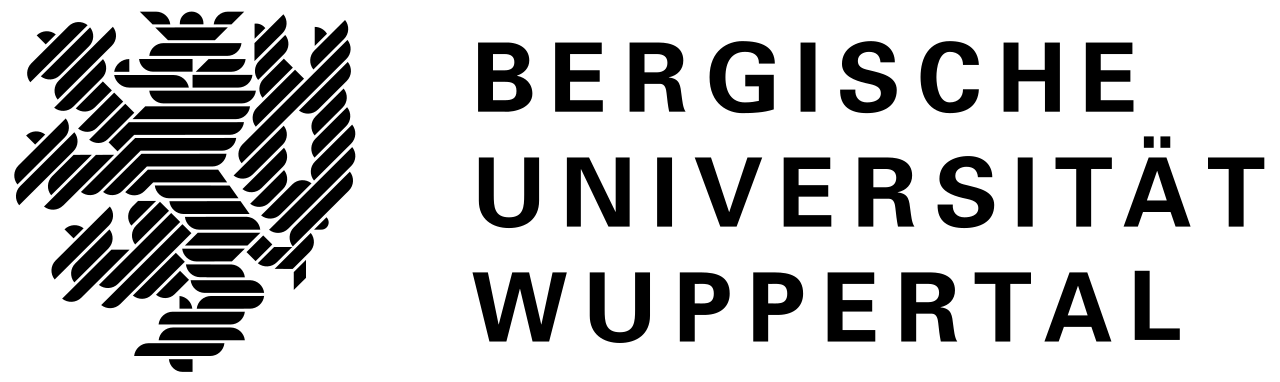
\includegraphics[width = 100mm]{BUW_Logo.svg.png}\\[8ex]
%     {\Huge \@title }\\[4ex]
%     {\Large  \@author}\\[4ex] 
%     \@date\\[8ex]
% \end{center}}
% \makeatother
\title{Title Page}
% \title{Lane Formation in Pedestrian Dynamics Simulations: \linebreak A Stochastic Port-Hamiltonian Approach}
% \author{Rafay Nawaid Alvi [2132500]}

\renewcommand{\figureautorefname}{Fig.}
\renewcommand{\equationautorefname}{Eq.}
\renewcommand{\tableautorefname}{Tab.}
\renewcommand{\subsectionautorefname}{Section.}
\renewcommand{\sectionautorefname}{Section.}
\providecommand*{\listingautorefname}{Code.}
% \renewcommand{\lstlistingname}{Code.}
% \renewcommand{\lstlistlistingname}{List of \listingname s.}
\SetupFloatingEnvironment{listing}{name=Code}
\SetupFloatingEnvironment{listing}{listname={List of Codes}}
\def\d{\mathrm d}
\def\L{\mathcal L}

% \renewcommand{\listingautorefname}{Code.}

% \renewcommand{\arraystretch}{1.5}

\addbibresource{bibliography/sample.bib}
% \input{figures/figures_tikz.tex}

\setlength{\parindent}{0in}
%\date{July 2023}
% \doublespace
\numberwithin{equation}{section}
\numberwithin{figure}{section}
\numberwithin{listing}{section}
\begin{document}
\begin{titlepage}
    \begin{center}
        % \vspace*{1cm}
        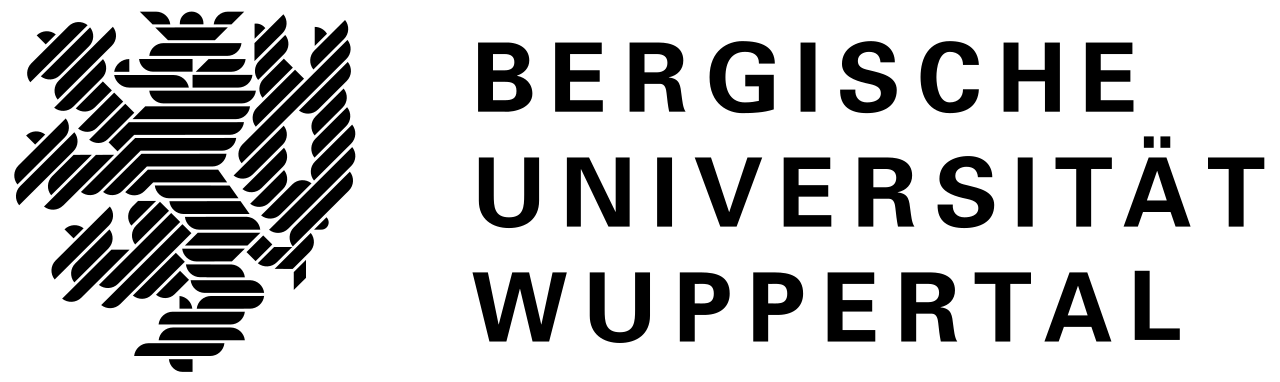
\includegraphics[width=90mm]{BUW_Logo.svg.png}

        \vspace*{0.5cm}
        \rule{\textwidth}{2pt}
        \LARGE
        \textbf{Lane Formation in Pedestrian Dynamics Simulations:}

        \textbf{A Stochastic Port-Hamiltonian Approach}
        \rule{\textwidth}{2pt}

        \vspace{0.5cm}
        \LARGE
        \textbf{Master's Thesis}

        \vspace{0.1cm}
        \large
        by

        % \vspace{0.1cm}
        \huge
        \textbf{Rafay Nawaid Alvi}
        \vfill

        % \vspace{0.5cm}
        \LARGE
        \textbf{Master's Program}\\
        \vspace{0.2cm}
        \Large
        \textbf{Computer Simulation in Science}

        \vspace{0.5cm}
        \Large
        Faculty of Mathematics and Natural Science \linebreak Bergsiche Universität Wuppertal

        \vspace{1cm}
        \textbf{Supervisors}\\
        \Large
        Prof. Dr. Antoine Tordeux \hfill Prof. Dr. Barbara Rüdiger
        \vfill
        \large
        \textbf{\today}
    \end{center}
\end{titlepage}
\pagebreak
\section*{Acknowledgement}

I am thankful to my supervisors Antoine Tordeux and Barbara Rüdiger, for their active support throughout the course of the thesis, and also for giving me an opportunity to embrace my curious endeavors by introducing this fascinating subject. I would also like to express my gratitude to the professors in computer simulation in science program for their lectures; in particular Lukas Arnold and Tristan Hehnen for their career advice and support throughout my university years.

A special thanks to my family as well as my small group of close friends, who've always been there with me through thick and thin, namely Muhammad Faisal Jamali, Dhruv Patel, Haider Hussain, Qendresa Buzolli, A. Raihan Bhuyian, and Zain Ul Haq Ansari. Their constant support and love were invaluable in helping me remain motivated.
\pagebreak
\tableofcontents
\pagebreak
\section{Overview}

% introduction and overview
% \section{Motivation}
\begin{frame}
    \frametitle{Overview}
    \begin{itemize}
        \item Study of collective behavior
        \item from microscopic force-based pedestrian models
        \item using Port-Hamiltonian Framework
        \item with stochastic elements
    \end{itemize}
\end{frame}
    
% \begin{frame}{Collective Behavior}{Macroscopic Behaviour}
%     In the context of Pedestiran Dynamics
%     \begin{itemize}
%         \item<1-> Counter Flow
%         \item<2-> Cross Flow
%     \end{itemize}
    
% \end{frame}


% \begin{frame}
%     \centering
%     \animategraphics[loop,autoplay,width=4cm]{20}{to_png/counterflow/frame-}{0}{273}
% \end{frame}

\begin{frame}{Collective Behavior}{Macroscopic Behaviour}
    \begin{columns}[t]
\begin{column}{0.48\linewidth}
    \centering
    Counter Flow: \linebreak Lane Formation \linebreak \linebreak
    \animategraphics[loop,autoplay,width=5cm]{25}{to_png/counterflow/frame-}{10}{273}
\end{column}
\begin{column}{0.48\linewidth}
    \centering
    Cross Flow: \linebreak Stripe Formation \linebreak \linebreak
    \animategraphics[loop,autoplay,width=5cm]{25}{to_png/crossflow/frame-}{10}{273}
\end{column}
    \end{columns}    
\end{frame}
%asuming you images are called "something-0.png" up to "something-16.png" 
% \begin{frame}
%     \transduration<0-100>{0}
%     \multiinclude[<+->][format=png, graphics={width=4cm}]{to_png/counterflow/frame}
% \end{frame}
\pagebreak
\section{Microscopic Pedestrian Model}

We will first construct the pedestrian model focusing on the interaction of agents to each other i.e. in the microscopic scale. In contrast, the macroscopic scale would focus on the resulting dynamics of the agents' interactions as a collective, which will be presented in more detail in the next section.

\subsection{Pedestrian Attributes}
Let us first start by describing our model. We follow the approach presented in \cite{tordeux2022multi} which follows a general class of microscopic force-based models approach given in \cite{helbing1995social,chraibi2011force}. The pedestrians exist on a toroidal surface, in other words, our model has periodic boundaries. For simplicity, the mass for all pedestrians is set to 1, hence their momentum $p_i$ is equal to the velocity, i.e. $p_i = m_i v_i = v_i$. The pedestrians also posses a desired velocity, which is assigned to each of them as an input to the model, this directs the pedestrians to desire a certain direction to move towards during the simulation run.

Given a pedestrian $i$ in $\mathbb{R}^2$ and time $0\leq t \leq T$, it possesses the following attributes:
\begin{itemize}
    \item Desired velocity: $u_i(t): [0,T] \mapsto \mathbb{R}^2$ 
    \item Current velocity: $p_i(t): [0,T] \mapsto \mathbb{R}^2$
    \item Current position: $q_i(t): [0,T] \mapsto \mathbb{R}^2$
\end{itemize} 
\begin{listing}[!ht]
\begin{minted}[escapeinside=??, frame=single]{julia}
## Define Agent
using Agents
@agent struct Pedestrian(ContinuousAgent{2,Float64})
    u?\sub{i}?::Vector{Float64} # Desired Velocity
end
\end{minted}
\caption{Defining the pedestrian agent in Julia's Agents.jl package. It is to be noted that \texttt{ContinuousAgent} specifies that our Pedestrian is a continuous agent with predefined position and velocity attributes constructed within the \texttt{@agent} macro. We only need to declare additional attributes such as \texttt{u}\sub{i}} 
\label{code:agent_def}
\end{listing}

For a model with $N \geq 2$ pedestrians, the relative position $\dot Q_{ij}(t)$ of a pedestrian $i$ to pedestrian $j$ is denoted as follows
\begin{align*}
    {Q}_{ij}(t) = q_i - q_j
\end{align*}
The vector of relative positions $Q_i(t)$ of a pedestrian $i$ to all pedestrians $j \neq i$ is denoted as follows
\begin{align*}
    {Q}_{i}(t) = ({Q}_{ij}(t))_{i\neq j} : [0,T] \mapsto \mathbb{R}^{2\cdot(N-1)} \text{ for } j = 1,\dots, N, \quad j \neq i
\end{align*}


\subsection{Microscopic Model Dynamics}
\label{section:micro_model_dynamics}
The dynamics of the pedestrians are based on (i) short-range repulsion $U$ among pedestrians based on their distances from others and (ii) attraction $\lambda$ toward a desired velocity $u_i$. The microscopic dynamics for the pedestrian $i$ is given by the following equations:
\begin{equation}
\begin{aligned}
    \dot Q_{ij}(t) &= p_i(t) - p_j(t), &j = 1,\dots,N \quad j \neq i& & \dot Q_i(0) &= Q^0_i \\
    \dot p_i(t) &= \lambda(u_i(t) - p_i(t)) - \sum_{j \neq i} \nabla U (Q_{ij}(t)), && & \dot p_i(0) &= p^0_i
\end{aligned}
\label{eq:micro}
\end{equation}
Here,
\begin{itemize}
    \item $\lambda \in \mathbb{R}_{\geq 0}$, is a parameter for the relaxation rate. In other words, it determines the intensity to reach the desired velocity. 
    \item $U(Q_{ij})$, is a nonlinear repulsive interaction potential, such that it is always positive and convex. This determines the magnitude of repulsion of a pedestrian $i$ to other pedestrians $j$ as a function of relative position $Q_{ij} = q_i - q_j$. It is defined as follows 
    \begin{align} 
        U(x) : \mathbb{R}^2 \mapsto \mathbb{R}, \quad\quad U(x) = ABe^{-|x|/B}
        \label{eq:def_potU}
    \end{align}
    Here, $|\cdot|$ is the minimum euclidean distance on the torus. $A$ and $B$ are scalar-valued parameters for the repulsion strength and the range of interaction respectively. Note that $U(x)$ is an even function, such that $\forall x \in \mathbb{R}^n, U(-x) = U(x)$. 
\end{itemize}

Hence, $\nabla U(x):\mathbb{R}^2 \mapsto \mathbb{R}^2$ is defined as
\begin{align} 
    \nabla U(x) = -A\dfrac{x}{|x|}e^{-|x|/B} = -\nabla U(-x)
    \label{eq:def_U}
\end{align}
It can be seen that this parameter is responsible for avoiding collisions between pedestrians, ensuring that the repulsive forces increase in magnitude the closer a pedestrian is. The underlying assumption is that the repulsive forces are a function of distance only. This is adapted from the concept of social forces and how they are determined from the surroundings of pedestrians. Also, note that $\nabla U(x)$ is an odd function.

Using the product rule, the Hessian $\mathbf{H}_U = \nabla ^2 U(x):\mathbb{R}^2 \mapsto \mathbb{R}^{2\times2}$ can be expressed as:
\begin{align}
    \mathbf{H}_U &= \nabla^2 U(x) = -A\left(\dfrac{x}{|x|}\dfrac{\d}{\d x} \left[ e^{-|x|/B} \right] + e^{-|x|/B}\dfrac{\d}{\d x} \left[\dfrac{x}{|x|}\right]\right) \nonumber \\ 
    &= \nabla^2 U(x) = -A\left[\dfrac{1}{|x|}\left(I - \dfrac{xx^T}{|x|^2}\right) - \dfrac{1}{B}\dfrac{xx^T}{|x|^2}\right]e^{-|x|/B}
    \label{eq:def_ddU}
\end{align}

Which will be used to evaluate the stochastic derivative in \autoref{section:stoch_derivative}

\subsection{Stochastic Model Dynamics}

To study the stochastic variant of our model, and how they effect the overall dynamics, we will introduce stochastic terms into our model. Generally a typical stochastic differential equation (SDE) is of the form
\begin{equation*}
    \d X_t = \underbrace{f(X_t, t)\d t}_{\text{drift}} + \underbrace{g(X_t, t)\d W_t}_{\text{diffusion}}
\end{equation*}
Which is a combination of a deterministic component, denoted as the \textit{drift} term; and a stochastic component, denoted as the \textit{diffusion} term. In our case, we introduce an additive noise term $\sigma dW_i(t)$ to our deterministic model from before \autoref{eq:micro} resulting in \autoref{eq:stoch_micro}. To be able to have a better physical interpretation of the model, the noise is introduced in the momentum term, rather than the position term. So one can interpret this as agents moving randomly while maintaining a continuous motion, as opposed to randomly teleporting in different locations at every time-step.
\begin{gather}
\begin{aligned}
    \d Q_{ij}(t) &= (p_i(t) - p_j(t))\d t \\
    \d p_i(t) &= \lambda(u_i(t) - p_i(t))\d t - \sum_{j \neq i} \nabla U (Q_{ij}(t))\d t + \sigma \d W_i(t)
    \label{eq:stoch_micro}
\end{aligned}
\end{gather}

The equation is reminiscent of a typical SDE with the first two terms being the deterministic part of the equation, i.e. drift and the last term being the stochastic part, i.e. the diffusion term. The randomness is induced via the Wiener process $(W_i(t))^N_{i=1}: [0,\infty) \times \Omega \rightarrow \mathbb{R}^N$, which is a mathematical description of the Brownian motion, that generates a sequence of random variables defined on a probability space $(\Omega, F, P)$ with independent increments \cite{oksendal2003stochastic}. Here, $\Omega$ is the sample space, $F$ the event space, and $P$ the probability measure. The stochastic term is amplified by the constant $\sigma \in \mathbb{R}$, which is often denoted as the volatility or diffusion coefficient.


\subsection{Identifying Collective Phenomenon}
With the dynamics presented so far, we can observe the individual pedestrian's attributes change over time. However, to identify whether a collective phenomenon is occurring we have also constructed a simple formula to measure the mean direction of all agents relative to their desired velocity direction, i.e. direction alignment $\phi$.

To measure how much an agent $i$ is moving in the direction of its particular desired velocity $u_i$, we can take the following dot product.
\begin{gather}
    \phi_i = \dfrac{p_i}{|p_i|} \cdot \dfrac{u_i}{|u_i|}, \quad \phi \in \mathbb{R}, \quad \phi \in [-1,1]
\end{gather}
The range of $\phi$ is $[-1, 1]$, with 1 indicating that the pedestrian is moving exactly in its desired direction, -1 indicating that the pedestrian is moving exactly opposite to its desired direction, whereas 0 indicates that it is either not moving or it is moving perpendicular to its desired speed. We can use this measure to quantify the mean direction of all agents. In other words, how aligned the mean direction of all agents is to their desired direction.
\begin{align}
    \text{Alignment} &= \dfrac{1}{N}\sum_{i=1}^N \phi_i \nonumber \\
    &= \dfrac{1}{N}\hat p^T \hat u
    \label{eq:alignment}
\end{align}
This will be useful, as we will later see, in identifying ordered and disordered collective dynamics. From a collective point of view, we can say that the value near 1 or -1 will indicate orderly behavior, signalling that all pedestrians are moving in their respective desired directions. Whereas values near 0 will indicate disorder.

\textbf{Calculation of Alignment}

In our simulations, we can take advantage of the fact that $u_i$ is always going to be a unit vector, i.e. either $[1,0]$, $[0,1]$, or $[0,0]$. Thus, we only use the unit vector of the velocity in the calculation of the alignment from \autoref{eq:alignment}, as shown in the code below.

\begin{listing}[H]
\begin{minted}[escapeinside=@@, frame=single, fontsize=\small]{julia}    
function calc_alignment(model)
    return mean(
        [transpose(i.vel/norm(i.vel))*(i.@u\sub{i}@) for i in allagents(model)]
        )
end
\end{minted}
\caption{Calculation of Mean direction of all pedestrians}
\label{code:calc_alignment}
\end{listing}

The benefit of this measure is made apparent in \autoref{plot:align_uni}. Here, we see how the mean direction of all the pedestrians gradually aligns with their desired velocity direction as the value moves from 0 to 1, showing the presence of order in the system.
\begin{figure}[H]
    \centering
    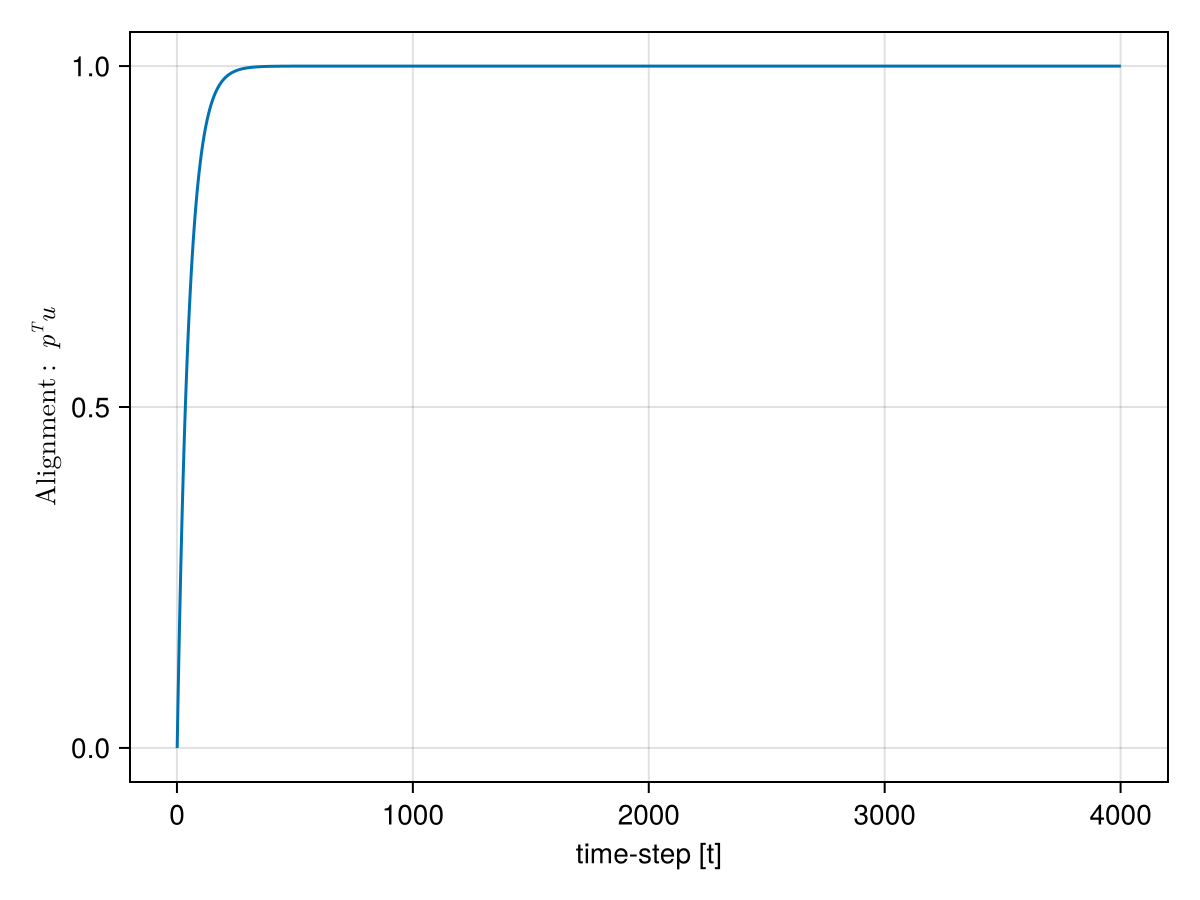
\includegraphics[width=0.49\linewidth]{figures/ch4_uniflow/straight_uni.png}
    \caption{Alignment for unidirectional flow.}
    \label{plot:align_uni}
\end{figure}

Through this measure, we can witness a shift from order to disorder by means of pedestrians aligning with their respective desired direction. Examples of this with various other cases will be shown in \autoref{section:observations}.
\pagebreak
\section{Port-Hamiltonian Formulation of the Microscopic Model}

This section serves to represent the microscopic dynamics of our pedestrian model using the framework of port-Hamiltonian systems, the generalized finite-dimensional PH formulation is given as:
\begin{equation}
\begin{aligned}
    \dot z(t) &= (J-R)\nabla H(z(t)) + Bu(t) \\
    y(t) &= B^T \nabla H(z(t))
\end{aligned}
\label{eq:ph_generalized}
\end{equation}

\subsection{Preliminaries}
Given a port-Hamiltonian System (PHS), such as the one defined in \autoref{eq:ph_generalized}, it is able to gain energy from or dissipate energy to other interacting systems. Here, $z$ is the state of the system, $u$ is the input, and $y$ is the output of the system. Furthermore, $J \in \mathbb R^{n \times n}$ is a skew-symmetric matrix, $R \in \mathbb R^{n \times n}$ is a positive semi-definite matrix that represents dissipation from the system, and $B \in \mathbb R^{n \times m}$ where $ m \ll n$ being the coefficient for the input.

One can achieve the classical Hamiltonian representation by assuming a system with no input, i.e. $B = 0$, and  no dissipation $R = 0$ as shown below using the first equation from \autoref{eq:ph_generalized}
\begin{gather*}
    \begin{aligned}
    \dot z(t) &= J \cdot \nabla H \\
    \begin{bmatrix}
        \dot q(t) \\ \dot p(t)
    \end{bmatrix}
    &=
    \begin{bmatrix}
        0 & I_n \\ 
        -I_n & 0
    \end{bmatrix}
    \begin{bmatrix}
        \partial H / \partial q \\
        \partial H / \partial p
    \end{bmatrix} 
    \end{aligned}
\end{gather*}
By setting the block matrices $I$ to size $n=1$, it can be demonstrated that the above equations yield the classical Hamiltonian equations, signifying that the skew-symmetry of $J$ is responsible for the conservation of the system.
\begin{align*}
\dot q = \dfrac{\partial H}{\partial p}, \quad \dot p = -\dfrac{\partial H}{\partial q}
\end{align*}
Having $R > 0$ allows the system to dissipate energy and the input $u$ allows the system to gain energy. As the inputs and outputs allows the system to interact with other systems, these can be denoted as ports of the system.

\subsection{Port-Hamiltonian Model}
For a system representing the microscopic model of $N > 2$ pedestrians, the state $z(t)$ would contain the relative positions and velocities of all pedestrians at a given time: $z(t) = (Q,p)^T$, where $Q = (Q_1,\dots,Q_N)$ and $p = (p_1,\dots,p_N)$ are vectors of relative positions and velocities of all pedestrians respectively. Such a system, as shown in \autoref{eq:micro} can be described through port-Hamiltonian formulation presented in \autoref{eq:ph_generalized} as follows:

\begin{equation}
    \begin{aligned}
        \dot z(t) &= (J-R)\nabla H(z(t)) + \lambda \tilde u(t), &\qquad z(0) = (Q^0,p^0)\\
        y(t) &= \lambda \nabla H(z(t)) 
    \end{aligned}
    \label{eq:ph_model}
\end{equation}

Here,
\begin{gather}
    \dot z(t) = 
    \begin{bmatrix}
        Q_1 & \cdots & Q_N & p_1 & \cdots & p_N 
    \end{bmatrix}^T
    \\
    \tilde u = \begin{bmatrix} 0 & \cdots & 0 & u_1(t) & \cdots & u_N(t) \end{bmatrix}^T
    \\
    J =
    \begin{bmatrix}
        0 & M \\
        -M^T & 0 
    \end{bmatrix},
    \quad 
    R =
    \begin{bmatrix}
        0 & 0 \\
        0 & \lambda I
    \end{bmatrix},
    \quad
    M = 
    \begin{bmatrix}
        M_1 \\ \vdots \\ M_N
    \end{bmatrix}
    \label{eq:JRM}
\end{gather}
The resulting system is a linear input-state-output port-Hamiltonian system with dissipation. The Hamiltonian can now be defined as the total energy of the system, i.e. the sum of kinetic and potential energies
\begin{align}
    H(z(t)) = \dfrac{1}{2}||p(t)||^2 + \dfrac{1}{2}\sum_{i=1}^N\sum_{j=1}^NU(Q_{ij}(t))
    \label{eq:Hamiltonian}
\end{align}
The gradient of the Hamiltonian would then be
\begin{gather}
    \nabla H = 
    \begin{bmatrix}
        \partial H / \partial Q \\ \partial H / \partial p
    \end{bmatrix}
    \label{eq:Hamiltonian_partial}
\end{gather}

The matrix equation representation of \autoref{eq:ph_model} can be written as
\begin{gather}
    \begin{bmatrix}
        \dot Q \\ \dot p
    \end{bmatrix} =
    \left(
    \begin{bmatrix}
        0 & M \\ 
        -M^T & 0
    \end{bmatrix} -
    \begin{bmatrix}
        0 & 0 \\
        0 & \lambda I
    \end{bmatrix} \right)
    \begin{bmatrix}
        \frac{1}{2} \nabla U(Q) \\
        p 
    \end{bmatrix}
    + \lambda 
    \begin{bmatrix}
        0 \\ u
    \end{bmatrix}
    \label{eq:matrixeq_ph}
\end{gather}


The block matrix $M$ can be defined such that 
\begin{equation}
\begin{aligned}
    \dot Q = Mp
\end{aligned}
\label{eq:Qmp}   
\end{equation}
with its elements
\begin{gather}
    M_1 = 
    \begin{bmatrix}
        1 & -1 & 0 & 0 & \dots & 0 \\
        1 & 0 & -1 & 0 & \dots & 0 \\
        \vdots & & &  &  & \vdots \\
        1 & & & &  & -1 \\
    \end{bmatrix}, \quad
    M_2 = 
    \begin{bmatrix}
        -1 & 1 & 0 & 0 & \dots & 0 \\
        0 & 1 & -1 & 0 & \dots & 0 \\
        \vdots & \vdots & &  &  & \vdots \\
        0 & 1& & &  & -1 \\
    \end{bmatrix}, \quad \dots
    \label{eq:M_n_def}
\end{gather}
 
%  which reiterates the previously established relationship between pedestrian $i$ and all pedestrians $j \neq i$,
%  \begin{equation*}\begin{aligned}
%     \dot Q_{i} = p_i - p_j
%  \end{aligned}
%  \label{eq:Qdot}
% \end{equation*}
\hrulefill

\textbf{R is positive semi-definite}

 One can show that $R$ is positive semi-definite by showing $x^TRx \geq 0$, where $x \in \mathbb R^n$ is a real-valued vector $ x = [x_1,\dots x_N]$:
 \begin{gather*}
    \begin{aligned}
    x^TRx&=x^T\begin{bmatrix}
        0 & 0 \\
        0 & \lambda I
    \end{bmatrix}x
    \\
    &=\begin{bmatrix}
        x_1\dots x_N
    \end{bmatrix}
    \begin{bmatrix}
        0 & 0 \\
        0 & \lambda I
    \end{bmatrix}
    \begin{bmatrix}
        x_1 \\ \vdots \\ x_N
    \end{bmatrix}
    \\
    &=\begin{bmatrix}
        0 & \lambda x_2 & \dots & \lambda x_N
    \end{bmatrix}
    \begin{bmatrix}
        x_1 \\ \vdots \\ x_N
    \end{bmatrix}
    \\
    &=\lambda(x_2^2+\dots+x_N^2) \geq 0
    \end{aligned}
 \end{gather*}
 Since $\lambda \geq 0$ and the squared terms are also positive, we can conclude that last expression as a whole is also greater than or equal to zero, proving that $x^TRx \geq 0$

 It can be observed that the parameter $\lambda$ is present in both the dissipation term $R$ and the coefficient term of the input $\tilde u$.
 
\hrulefill

\textbf{Example: $N=3$}

To better illustrate the implementation of the model, here we will concretely show the formulation of the model using $N=3$ pedestrians. Here the matrix $M = (M_1, M_2, M_3)^T$, where each $M_i$ shows the difference in quantities with respect to the pedestrian $i$ as shown below.

\begin{gather*}
    M_1 = 
    \begin{bmatrix}
        1 & -1 & 0 \\
        1 & 0 & -1 
    \end{bmatrix},\;
    M_2 = 
    \begin{bmatrix}
        -1 & 1 & 0 \\
        0 & 1 & -1 
    \end{bmatrix},\;
    M_3 = 
    \begin{bmatrix}
        -1 & 0 & 1 \\
        0 & -1 & 1 
    \end{bmatrix}
\end{gather*}

It can be observed that $M$ unfolds the relative velocities of pedestrians, resembling the dynamics presented in the first equation of \autoref{eq:micro}
% \end{column}
% \begin{column}{0.5\textwidth}
\begin{gather*}
    M = 
    \begin{bmatrix}
        M_1 \\ 
        M_2 \\
        M_3
    \end{bmatrix}, \qquad
    \dot Q = Mp = 
    \begin{bmatrix}
        p_1 - p_2 \\
        p_1 - p_3 \\
        p_2 - p_1 \\
        p_2 - p_3 \\
        p_3 - p_1 \\
        p_3 - p_2 
    \end{bmatrix}
\end{gather*}
Lastly, we represent the Hamiltonian
\begin{gather*}
    \begin{aligned}
        H = \frac{1}{2}(p_1^2 + p_2^2 + p_3^2) + \frac{1}{2}(&\nabla U_{12} + \nabla  U_{13} + \\  
        &\nabla  U_{21} +\nabla  U_{23} + \\ 
        &\nabla  U_{31} +\nabla  U_{32})
    \end{aligned}    
\end{gather*}

\hrulefill

\subsection{Deriving the Equations of Motion}
We can show that the port-Hamiltonian formulation \autoref{eq:ph_model} is indeed the same model as \autoref{eq:micro} by deriving the latter from the former. 
Let us start by simplifying the matrix equation \autoref{eq:matrixeq_ph} for $\dot Q$ and $\dot p$

\begin{gather*}
    \dot Q = 
    \left[
    \begin{bmatrix}
        0 & M
    \end{bmatrix}
    - \begin{bmatrix}
        0 & 0
    \end{bmatrix}
    \right]
    \begin{bmatrix}
        \frac{1}{2}\nabla U(Q) \\
        p
    \end{bmatrix}
    +\lambda\begin{bmatrix}
        0
    \end{bmatrix}
\end{gather*}
\begin{gather*}
    \dot p= 
    \left[
    \begin{bmatrix}
        -M^T & 0
    \end{bmatrix}
    - \begin{bmatrix}
        0 & \lambda I
    \end{bmatrix}
    \right]
    \begin{bmatrix}
        \frac{1}{2}\nabla U(Q) \\
        p
    \end{bmatrix}
    +\lambda\begin{bmatrix}
        u
    \end{bmatrix}
\end{gather*}
Resolving $\dot Q$ would reiterate the relationship described in \autoref{eq:Qmp}
\begin{equation*}
    \dot Q = Mp
\end{equation*}
And, resolving $\dot p$ gives us the equation for the velocity in matrix form
\begin{equation*}
    \dot p = -M^T\frac{1}{2}\nabla U(Q) - \lambda p + \lambda u
\end{equation*}

Using the definition of $M$ from \autoref{eq:JRM} and \autoref{eq:M_n_def}, we can construct the equations for $Q$ for every $i = 1,\dots,N$.
\begin{align*}
    \dot Q_{ij} = p_i - p_j
\end{align*}
Similarly, using the property that $U(x)$ is an odd function \autoref{eq:def_U}, we can derive $\dot p$
\begin{align*}
    \dot p_i &= \lambda(u_i - p_i) - \frac{1}{2}\sum_{j \neq i}(\nabla U(Q_{ij}) - \nabla U(Q_{ji})) \\ 
    \dot p_i &= \lambda(u_i - p_i) - \sum_{j \neq i}\nabla U(Q_{ij}) 
\end{align*}

By showing the derivation of the same microscopic dynamics from the port-Hamiltonian formulation, we can establish that the proposed microscopic model for the pedestrian dynamics has Hamiltonian structure, and that the system can be described using the Hamiltonian $H$ as a quantitative measure for the collective dynamics of the pedestrians.

\subsection{Stochastic Port Hamiltonian Formulation}
Continuing from the stochastic induced dynamics of the microscopic model in \autoref{eq:stoch_micro}, we can use the port-Hamiltonian formulation of the deterministic dynamics \autoref{eq:ph_model} and represent it with the noise term.
\begin{equation}
    \begin{aligned}
        dz(t) &= (J-R)\nabla H(z(t))dt + \lambda \tilde u(t)dt + \sigma d\xi(t)\\
        dy(t) &= \lambda \nabla H(z(t))dt
    \end{aligned}
    \label{eq:stoch_ph_model}
\end{equation}
Similar to \autoref{eq:matrixeq_ph}, and following the formulation from \cite{rudiger2024stability}, the matrix equation representation would become
\begin{gather}
    \begin{bmatrix}
        dQ \\ dp
    \end{bmatrix} =
    \left(
    \begin{bmatrix}
        0 & M \\ 
        -M^T & 0
    \end{bmatrix} -
    \begin{bmatrix}
        0 & 0 \\
        0 & \lambda I
    \end{bmatrix} \right)
    \begin{bmatrix}
        \frac{1}{2} \nabla U(Q) \\
        p 
    \end{bmatrix}dt
    + \lambda 
    \begin{bmatrix}
        0 \\ u
    \end{bmatrix}dt
    + \sigma
    \begin{bmatrix}
        0 \\ dW(t)
    \end{bmatrix}
    \label{eq:matrix_stoc_eq_ph}
\end{gather}

This will be used as the basis of our stochastic system. Following from the dynamics presented in \autoref{eq:stoch_micro}, it can be noted that the stochastic term is only effecting the momentum equation.

It can also be noted that the expression for the Hamiltonian \autoref{eq:Hamiltonian} will remain the same, since the stochastic terms are included within the momentum term $\dot p$. 

\subsection{Macroscopic Observations from Hamiltonian Behavior}
The time derivative of the Hamiltonian is derived by its taking the total derivative with respect to time:
\begin{align*}
    \dfrac{d}{dt}H(z(t)) = \nabla^T H(z(t))\cdot \dot z(t)
\end{align*}
Substituting $\dot z(t)$ from \autoref{eq:ph_model} denoting that $y = \lambda \nabla H$ and thus $y^T = \nabla^T H \lambda$, we get
\begin{align*}
    \dfrac{d}{dt}H(z(t)) = \nabla^T H(z(t))(J-R)\nabla H(z(t)) + \underbrace{\nabla^T H(z(t)) \lambda}_{y^T} \tilde u
\end{align*}
Using the skew-symmetric property of $J$ that $x^TJx=0$ we can simplify and obtain the expression for the time derivative of the Hamiltonian.
\begin{align}
    \frac{d}{dt}H(z(t)) = y^Tz(t)\tilde u(t) - \nabla^T H(z(t))R \nabla H(z(t))
\end{align}

Expanding the terms further by substituting the gradient of the Hamiltonian \autoref{eq:Hamiltonian_partial} and the definition of $R$ \autoref{eq:JRM} can help us further simplify the expression giving us the following energy balance
\begin{align}
    \dfrac{d}{dt}H(z(t)) &= \lambda \nabla^T H(z(t)) \tilde u - \nabla^T H(z(t)) R \nabla H(z(t)) \nonumber \\
    &\begin{aligned}
        &= \lambda 
        \begin{bmatrix}
        % \dfrac{\partial H}{\partial Q} & \dfrac{\partial H}{\partial p}
        \partial H / \partial Q & \partial H / \partial p
        \end{bmatrix}
        \begin{bmatrix}
            0 \\
            u
        \end{bmatrix}
        - 
        \begin{bmatrix}
            % \dfrac{\partial H}{\partial Q} & \dfrac{\partial H}{\partial p}
        \partial H / \partial Q & \partial H / \partial p
        \end{bmatrix}
        \begin{bmatrix}
            0 & 0 \\ 0 & \lambda I
        \end{bmatrix}
        \begin{bmatrix}
            % \frac{\partial }{\partial Q} H \\ \frac{\partial }{\partial p}H
        \partial H / \partial Q \\ \partial H / \partial p
        \end{bmatrix}  \\ 
        &= \lambda p^T u - \lambda  p^T p \\ 
        &= \lambda p^T (u - p) \\ 
    \end{aligned} \nonumber \\
    \dfrac{d}{dt}H(z(t))&= \lambda \langle p(t),u(t)-p(t) \rangle
    \label{eq:dH}
\end{align}


It can be seen that the time derivative of the Hamiltonian $\frac{d}{dt}H(z(t))$ depends only on the velocities of the pedestrians.

With this, we can confirm the following claims
\begin{itemize}
    \item The Hamiltonian remains constant $\frac{d}{dt}H(z(t)) = 0$ for all times $t \geq 0$ if the system has no dissipation $\lambda = 0$. 
    \begin{align*}
        \forall t \geq 0,\quad \dfrac{d}{dt}H(z(t)) = 0 \qquad \text{if} \qquad \lambda = 0
    \end{align*}
    Reiterating that purely Hamiltonian behavior is indeed conservative.
    \item If the desired velocities are zero, i.e. $u = 0$, then the Hamiltonian decreases over time
    \begin{align*}
        \forall t \geq 0,\quad \dfrac{d}{dt}H(z(t)) \leq 0 \qquad \text{if} \qquad \forall i,\; u_i = 0
    \end{align*}
    Since the system is allowed to dissipate without input feed, the asymptotic behavior would yield crystallization, i.e. the pedestrians would stop moving.
    \item If all the pedestrians move at their desired velocities, i.e. $p(t) = u(t)$, then the time derivative is zero
    \begin{align*}
        \dfrac{d}{dt} H(z(t) = 0 \qquad \text{if} \qquad \forall i,\; p_i(t) = u_i(t)
    \end{align*}
\end{itemize}
\pagebreak
\section{Numerical Schemes and Simulation}
After establishing that the dynamics of our microscopic model possesses Hamiltonian structure, we can now show these dynamics in action through simulations. In this section we will compare three numerical schemes: explicit Euler, implicit Euler, and Leapfrog, how they are constructed for our model; and how they compare with each other. Furthermore, we construct a solver using the implicit Euler-Maruyama scheme for the stochastic port-Hamiltonian case. For the simulation, the following JuliaLang packages are extensively utilized, \texttt{Agents.jl} and \texttt{DifferentialEquations.jl}.

\subsection{Model Setup}
The simulation is run on a fixed model setup as shown in \autoref{code:model_init}. Here we initialize the values for the number of pedestrians, the extent of the domain in 2D, the desired velocities of the pedestrians, and the parameter values of $\lambda$, $A$, $B$, and $\sigma$.
\begin{table}[H]
    % \centering
    \begin{tabular}{lc}
        Pedestrian Sensitivity: & $\lambda = 2$ \\
        Desired Speed: & $|u| = 1$ \\
        Repulsion Strength: & $A = 5$ \\
        Interaction Range: & $B = 0.3$ \\
        Volatility: & $\sigma = 0.0$
    \end{tabular}
\end{table}
These parameter values are chosen to replicate the results from \cite{tordeux2022multi}, which follows the works of \cite{helbing1995social,tordeux2016collision}. For the stochastic case, we replicate the results from \cite{khelfa2021initiating}. The volatility coefficient $\sigma$ is only relevant for stochastic cases -- as we will see in later sections, whereas in deterministic cases it remains zero.

\begin{listing}[H]
\begin{minted}[escapeinside=??,frame=single, fontsize=\small]{julia}
properties = Dict(
    :?\textlambda? => 2, 
    :A => 5,
    :B => 0.3, 
    :dt => 0.01,
    :?\textsigma? => 0.0,
    :Hamiltonian => 0.0,
    :dH => 0.0
)
number_of_peds = 32 # number of pedestrians
x_len = 11 # domain length in x
y_len = 5 # domain length in y
seed = 42
model = initialize(number_of_peds, x_len, y_len, leapfrog_step, properties,
                   seed)
\end{minted}
\caption{Initialization of the model}
\label{code:model_init}
\end{listing}
The \texttt{initialize} function shown in \autoref{code:model_init} initializes the model with the given parameters. It also utilizes the functionalities provided by the \texttt{Agents.jl} package shown in \autoref{code:model_param} such as \texttt{ContinuousSpace} and \texttt{StandardABM}.
\begin{listing}[H]
\begin{minted}[escapeinside=??, frame=single, fontsize=\small]{julia}
space = ContinuousSpace((x_len, y_len); periodic = true)
model = StandardABM(
    Pedestrian,
    space;
    model_step! = (model) -> model_step!(model, num_solver),
    properties,
    rng # random number generator
)
\end{minted}
\caption{Inside the \texttt{initialize} function from \autoref{code:model_init}, showing that \texttt{ContinuousSpace} method takes care of the space as well as the periodic boundaries}
\label{code:model_param}
\end{listing}


The argument \texttt{num\_solver} is used to specify an ODE solver. As an example \autoref{code:model_init} uses \texttt{leapfrog\_step} from \autoref{code:leapfrog} as a solver. The construction of which is discussed in \autoref{section:numerical_schemes}. Additionally, one can construct other methods to be used in place of \texttt{num\_solver}, such methods can be constructed using the solvers provided by the \texttt{DifferentialEquations.jl} package. These powerful solvers are used for complex scenarios such as solving SDEs (Stochastic Differential Equations) as will be discussed later in this section.

Once the model is initialized, it places the specified number of pedestrians randomly on the grid \autoref{code:agent_init}. Here \texttt{rng} makes use of a Random Number Generator with a specified \texttt{seed} that remains fixed for the model. This is done so that simulation results can be replicated.

\begin{listing}[H]
\begin{minted}[escapeinside=??, frame=single, fontsize=\small]{julia}
for i in 1:number_of_peds
    add_agent!(model;
        pos = [rand(rng)*x_len, rand(rng)*y_len],  # Initial position
        vel = [0.0,0.0], # Initial velocity
        u?\sub{i}? = [1.0,0.0] # uni-directional flow
        # u?\sub{i}? = mod(i,2) == 0 ? [1,0] : [-1,0] # counter_flow
        # u?\sub{i}? = mod(i,2) == 0 ? [0,1] : [1,0] # cross_flow
    )
end
\end{minted}
\caption{Code snippet inside \texttt{initialize}, here every pedestrian is initialized with a position in the space and a desired velocity (\texttt{u}\sub{i}). It can be seen that we can customize the desired velocities to initiate counter flow and cross flow. }
\label{code:agent_init}
\end{listing}

We can also now define a \texttt{model\_step!} function \autoref{code:model_step} that can be used to run our model. At each time-step of the simulation this \texttt{model\_step} takes in the results of the solver used for every agent and modifies the values of each agent. It also calculates the Hamiltonian and its time derivative at each step which are defined in \autoref{section:calc_ham}
\begin{listing}[H]
\begin{minted}[escapeinside=??, frame=single, fontsize=\small]{julia}
function model_step!(model,num_solver)
    for agent in allagents(model)
        v, p = num_solver(agent,model)
        p = normalize_position(p,model) # for periodic boundaries
        agent.vel = v
        agent.pos = p
    end
    model.hamiltonian = calc_hamiltonian(model)
    model.dH = calc_dH(model)
end
\end{minted}
\caption{At each step simulation of the model, \texttt{model\_step!} updates the model parameters as well as the agent parameters.}
\label{code:model_step}
\end{listing}


\subsection{Construction of Numerical Schemes}
\label{section:numerical_schemes}

It is well-established that the preferred numerical methods for Hamiltonian systems are the symplectic methods. These methods are designed such that they preserve the Hamiltonian structure, in other words, they take into account the conservation of energy and hence are better to suited to solve physical systems.

For every pedestrian $i$, the numerical schemes solve for two equations: the positions $q^{k+1}$ and velocities $p^{k+1}$ at time-step $\delta \text{t}$. We recall our dynamic equations from \autoref{eq:micro}, however we write it a bit differently.
\begin{gather}
    \begin{aligned}
    \dot p_i &= a(q_i,p_i) \\
    \dot q_i &= p_i
    \end{aligned}
    \label{eq:diff_pq}
\end{gather}
For clarity, we emphasize the acceleration function and denote it as $a_i(q,p)$ \autoref{eq:acc}. We use this representation to illustrate the numerical methods used.
\begin{equation}
    a_i(q,p) = \lambda(u_i - p_i) - \sum_{j \neq i} \nabla U(q_i - q_j)
    \label{eq:acc}
\end{equation}
In \autoref{code:acc} we define the acceleration function, however we first construct a function \texttt{dU} in \autoref{code:dU} to calculate an interaction potential given the positions \texttt{(pos1, pos2)} of a pair of pedestrians, this is needed in the second term of \autoref{eq:acc}, which sums all interaction potentials given the pedestrian $i$.
\begin{listing}[H]
\begin{minted}[escapeinside=??, frame=single, fontsize=\small]{julia}
function dU(pos1, pos2, model)
    A = abmproperties(model)[:A]
    B = abmproperties(model)[:B]
    dist = euclidean_distance(pos1, pos2, model)
    result = ((get_direction(pos1,pos2,model))/dist)*A*exp(-dist/B)
    return result
end
\end{minted}
\caption{Calculation of \texttt{dU} from \autoref{eq:def_U}. The \texttt{properties} defined in \autoref{code:model_param} can be extracted using \texttt{abmproperties}. The methods \texttt{euclidean\_distance}, and \texttt{get\_direction} are also from \texttt{Agents.jl}}
\label{code:dU}
\end{listing}

\begin{listing}[H]
    \begin{minted}[escapeinside=??, frame=single, fontsize=\small]{julia}    
function acc(pos::SVector{2,Float64}, vel::SVector{2,Float64}, agent, model)
    ?\textlambda? = abmproperties(model)[:?\textlambda?]
    val = ?\textlambda?.*(agent.u?\sub{i}? - vel) - 
          sum(
            dU(pos,i.pos,model) for i in allagents(model) 
            if i.id != agent.id
            )
    return val
end
\end{minted}
\caption{Implementation of \autoref{eq:acc}. The \texttt{allagents} function returns an iterator over all pedestrians in the model}
\label{code:acc}
\end{listing}
The numerical schemes can be a combination of different schemes for each of these equations. The methods used here are:
\begin{itemize}
    \item Explicit/Explicit Euler scheme:
    \begin{gather}\begin{aligned}
        p^{k+1} &= p^k + \delta\text{t} \; a(q^k,p^k) \\
        q^{k+1} &= q^k + \delta\text{t} \; p^k 
    \end{aligned}
    \label{eq:explicit_euler}
    \end{gather}
    \item Implicit/Implicit Euler scheme:
    \begin{gather}
        \begin{aligned}
        p^{k+1} &= p^k + \delta\text{t} \; a(q^{k+1},p^{k+1}) \\
        q^{k+1} &= q^k + \delta\text{t} \; p^{k+1}
    \end{aligned}
    \label{eq:impliict_euler}
    \end{gather}
    Given that this is an implicit method, i.e. $p^{k+1}$ exists on both the right and left side of the equation, $p^{k+1} = p^k + \delta\text{t} \; a(q^{k+1},p^{k+1})$ needs to be solved numerically for each time-step $\delta$t. 
    \item Leapfrog scheme:
    \begin{gather*}\begin{aligned}
        p^{k+1} &= p^k + \dfrac{\delta\text{t}}{2} \; \left(a(q^{k},p^{k})+a(q^{k+1},p^{k+1})\right) \\
        q^{k+1} &= q^k + \delta\text{t} \; p^k + \dfrac{\delta\text{t}^2}{2} \; a(q^{k},p^{k}) 
    \end{aligned}\end{gather*}
    It is to be noted that:
    \begin{equation}
        a(q^{k+1},p^{k+1}) = a(q^{k+1},p^{k}) + \lambda(p^k - p^{k+1})
        \label{eq:acc_relationship}
    \end{equation}
    the leapfrog scheme can be simplified to:
    \begin{gather}\begin{aligned}
        p^{k+1} &= p^k + \dfrac{\delta\text{t}}{2 + \delta\text{t}} \; \left(a(q^k,p^k) + a(q^{k+1},p^{k}) \right) \\
        q^{k+1} &= q^k + \delta\text{t} \; p^k + \dfrac{\delta\text{t}^2}{2} \; a(q^{k},p^{k})
        \label{eq:leapfrog}
    \end{aligned}\end{gather}
\end{itemize}


To demonstrate how these numerical methods are defined in code, we can see the implementation of leapfrog scheme in \autoref{code:leapfrog}. It can be noted that the explicit Euler can be defined similarly because both of these methods (\autoref{eq:explicit_euler} and \autoref{eq:leapfrog}) are explicit.

\begin{listing}[H]
\begin{minted}[escapeinside=??, frame=single, fontsize=\small]{julia}    
function leapfrog_step(agent::Pedestrian, model)
    acc_old = acc(agent.pos, agent.vel, agent, model)
    p = agent.pos + model.dt.*agent.vel + ((model.dt^2)/2).*acc_old
    p = normalize_position(p, model)
    acc_new = acc(p, agent.vel, agent, model)
    v = agent.vel + ((model.dt)/(2 + model.λ*model.dt)).*(acc_old + acc_new)
    return v, p
end 
\end{minted}
\caption{The leapfrog scheme \autoref{eq:leapfrog} in code}
\label{code:leapfrog}
\end{listing}

% \subsection{Using ODE solvers provided by \texttt{DifferentialEquations.jl}}
\textbf{Using ODE solvers provided by \texttt{DifferentialEquations.jl}}

To define implicit Euler method \autoref{eq:impliict_euler}, we make use of the package solvers. As per the directions of \texttt{DifferentialEquations.jl}, we first construct our \texttt{ODEProblem} based on the dynamics provided in \autoref{eq:diff_pq}
\begin{listing}[H]
\begin{minted}[escapeinside=@@, frame=single, fontsize=\small]{julia}    
function ph_model!(du,u,p,t)
    agent, model = p
    vel, pos = u[1:2], u[3:4]
    du[1:2] = acc(agent.pos, agent.vel, agent, model)
    du[3:4] = vel
end
\end{minted}
\caption{Defining \autoref{eq:diff_pq} as an \texttt{ODEProblem}}
\label{code:ph_prob}
\end{listing}

Next we define a solver function that integrates the ODE. Here, we provide the initial conditions \texttt{u0} as the pedestrians velocities and positions, and an integrator function that generates a solution for a single time-step \texttt{dt} using \texttt{step!}. This function can now be used as an argument for \texttt{initialize()} in place of \texttt{num\_solver} in \autoref{code:model_param}.
\begin{listing}[H]
\begin{minted}[escapeinside=@@, frame=single, fontsize=\small]{julia}    
function ode_step(agent, model)
    u0 = [agent.vel[1], agent.vel[2], agent.pos[1], agent.pos[2]]
    tspan = (0.0, Inf)
    p = (agent, model)
    prob = ODEProblem{true}(ph_model!, u0, tspan, p)
    
    # Use the model's integrator
    integrator = init(prob, ImplicitEuler(), dt=model.dt)
    
    # Solve and update agent state
    step!(integrator, model.dt)
    vel = integrator.u[1:2]
    pos = integrator.u[3:4]
    return vel, SVector{2}(pos)
end
\end{minted}
\caption{ODE solver function to solve the model defined in \autoref{code:ph_prob} as \texttt{ODEProblem}. Here, we have chosen the solver as \texttt{ImplicitEuler}}
\label{code:ph_solver}
\end{listing}

Similar to \texttt{ODEProblem} in \autoref{code:ph_solver}, one can also go a step further and define and solve a \texttt{DynamicalODEProblem} or \texttt{SDEProblem} using \texttt{DifferentialEquations.jl}. Since we are also interested in symplectic methods such as the \texttt{leapfrog}, it would also be important to be able to construct a solver for our dynamic problem as well. Here, in contrast to our previous approach, the only difference is that we define the equations for $\dot p$ and $\dot q$ separately, as shown in \autoref{code:ph_dyn_problem}
\begin{listing}[H]
\begin{minted}[escapeinside=@@, frame=single, fontsize=\small]{julia}    
function ph_p!(dv,v,u,p,t)
    agent, model = p
    vel = v[1:2]
    pos = u[1:2]
    dv[1:2] = acc(agent.pos, agent.vel, agent, model)
end
function ph_q!(du,v,u,p,t)
    agent, model = p
    vel = v[1:2]
    du[1:2] = vel
end
\end{minted}
\caption{Defining the \texttt{DynamicalODEProblem} using separate functions for $\dot p$ and $\dot q$}
\label{code:ph_dyn_problem}
\end{listing}
Furthermore, we explicitly separate the initial conditions for velocities and positions, and define the problem using \texttt{DynamicalODEProblem}. We use \texttt{VerletLeapfrog} as our solver as demonstrated in \autoref{code:ph_dyn_solver}.
\begin{listing}[H]
\begin{minted}[escapeinside=@@, frame=single, fontsize=\small]{julia}        
function dynamic_ode_step(agent, model)
    v0 = [agent.vel[1], agent.vel[2]]
    u0 = [agent.pos[1], agent.pos[2]]
    tspan = (0.0, Inf)
    p = (agent, model)
    prob = DynamicalODEProblem(ph_p!,ph_q!,v0,u0, tspan, p)
    
    # Use the model's integrator
    integrator = init(prob, VerletLeapfrog(), dt=model.dt)
    
    # Solve and update agent state
    step!(integrator, model.dt)
    vel = integrator.u[1:2]
    pos = integrator.u[3:4]
    return vel, SVector{2}(pos)
end
\end{minted}
\caption{Solving the model using \texttt{VerletLeapfrog}}
\label{code:ph_dyn_solver}
\end{listing}

This approach of using \texttt{DifferentialEquations.jl} to define and solve our model allows more flexibility to choose from a wider range of sophisticated solvers provided by the package. However, one concerning issue is that this solver uses leapfrog discretization in its original form that will still discretize the model as an implicit scheme, whereas previously, we used the convenient relationship provided by the formulation of the acceleration \autoref{eq:acc_relationship} to manipulate the original discretization to form an explicit leapfrog \autoref{eq:leapfrog}, which proved to be more beneficial as it provides the same results with less computational load.

To solve for the stochastic port-Hamiltonian case, we can make use of an SDE solver. We will first have to define our model as an \texttt{SDEProblem}. To do this, we will define the drift term and diffusion term separately as shown in \autoref{code:sde_problem}. This reflects the standard SDE form as described in \autoref{eq:stoch_micro}.

\begin{listing}[H]
    \begin{minted}[escapeinside=@@, frame=single, fontsize=\small]{julia}        
function ph_stoc_drift!(du,u,p,t)
    agent, model = p
    vel, pos = u[1:2], u[3:4]
    du[1:2] = acc(agent.pos, agent.vel, agent, model)
    du[3:4] = vel
end
function ph_stoc_diffu!(du,u,p,t)
    agent, model = p
    vel, pos = u[1:2], u[3:4]
    @\textsigma@ = model.sigma
    du[1:2] = [@\textsigma@,@\textsigma@] 
    du[3:4] = [0.0,0.0]
end
\end{minted}
\caption{Defining the \texttt{SDEProblem}}
\label{code:sde_problem}
\end{listing}

And finally, we construct our solver to be used as another stepping function for our simulation. It can be seen how the stochastic component is added as a Wiener Process. The solver used for most simulations in the next section is the implicit Euler-Maruyama, however other solvers are also provided the package such as the \texttt{SImplicitMidpoint} \cite{rackauckas2017differentialequations}. This provides room for reassessment on the choice for the solver to be used, specially in a case such as ours that demands symplectic solvers.
\begin{listing}[H]
    \begin{minted}[escapeinside=@@, frame=single, fontsize=\small]{julia}        
function stochastic_ode_step(agent, model)
    u0 = [agent.vel[1], agent.vel[2], agent.pos[1], agent.pos[2]]
    tspan = (0.0, Inf)
    p = (agent, model)
    W = WienerProcess(0.0, 0.0, 0.0)
    prob = SDEProblem(ph_stoc_drift!,ph_stoc_diffu!,u0, tspan, p, noise=W)
    
    # Use the model's integrator
    integrator = init(prob, ImplicitEM(), dt=model.dt)
    
    # Solve and update agent state
    step!(integrator)
    vel = integrator.u[1:2]
    pos = integrator.u[3:4]
    return vel, SVector{2}(pos)
end
\end{minted}
\caption{Solving the SDE using implicit Euler-Maruyama}
\label{code:sde_solve}
\end{listing}

To summarize, in this section we've devised mainly four solvers: for the deterministic port-Hamiltonian model, we have explicit Euler, implicit Euler, and leapfrog; for the stochastic port-Hamiltonian model, we have implicit Euler-Maruyama method. We have allowed ourselves further flexibility by introducing packaged solvers. For the upcoming simulations in the remainder of this section, we will be using \autoref{code:ph_solver} for the implicit Euler as well as explicit Euler by changing the solver to \texttt{Euler}; and \autoref{code:leapfrog} for the leapfrog. Next, we will formulate functions to calculate the Hamiltonian in our model, and then compare the results obtained by each solver.

\subsection{Calculation of Hamiltonian}
\label{section:calc_ham}

To compare these numerical schemes, we can of course observe how the agents interact over time and whether they reach a lane or stripe formation based on the provided desired velocity \texttt{u}\sub{i}. But to have a quantitative measure, we also would like to calculate the Hamiltonian \autoref{eq:Hamiltonian} and observe the change in Hamiltonian \autoref{eq:dH} over time. For this reason we included \texttt{:Hamiltonian} and \texttt{:dH} as key-value pairs in the \texttt{properties} dictionary from \autoref{code:model_init} and define functions \autoref{code:calc_hamiltonian} and \autoref{code:calc_dH} to calculate them.

\begin{listing}[H]
\begin{minted}[escapeinside=??, frame=single, fontsize=\small]{julia}    
function calc_hamiltonian(model)
    kinetic_energy = 0.5.*sum(
        [transpose(a.vel)*a.vel for a in allagents(model)]
        )
    potential_energy = 0.5.*sum(
        [sum_potU(a,allagents(model),model) for a in allagents(model)]
        )
    return kinetic_energy + potential_energy
end
\end{minted}
\caption{Calculation of Hamiltonian $H(z(t))$ as defined in \autoref{eq:Hamiltonian}. For clarity, the kinetic and potential terms are calculated separately. One can easily observe that the function \texttt{sum\_potU} evaluates the double summation.}
\label{code:calc_hamiltonian}
\end{listing}

\begin{listing}[H]
\begin{minted}[escapeinside=??, frame=single, fontsize=\small]{julia}    
function calc_dH(model)
    return sum(
        [model.?\textlambda?*norm(i.vel)*norm(i.u?\sub{i}? - i.vel) for i in allagents(model)]
        )
end
\end{minted}
\caption{Calculation of $\frac{d}{dt}H(z(t))$ as defined in \autoref{eq:dH}}
\label{code:calc_dH}
\end{listing}

Inner summation of the second term in \autoref{eq:Hamiltonian} is defined in the function \texttt{sum\_potU}. This simply adds all the individual potential energies between pairs of all combinations of the pedestrians in the model. The potential energy \autoref{code:sum_potU} is calculated following the definition provided in \autoref{eq:def_potU}
\begin{listing}[H]
\begin{minted}[escapeinside=@@, frame=single, fontsize=\small]{julia}    
function potU(a1::Pedestrian,a2::Pedestrian, model)
    A = model.A
    B = model.B
    dist = euclidean_distance(a1, a2, model)
    return A*B*exp(-dist/B)
end

function sum_potU(a1::Pedestrian, agents, model)
    return sum([i.id != a1.id ? potU(a1, i, model) : 0 for i in agents])
end
\end{minted}
\caption{Evaluating the inner summation of potential energies from \autoref{eq:Hamiltonian} using \texttt{sum\_potU} in the calculation of the Hamiltonian in \autoref{code:calc_hamiltonian}}
\label{code:sum_potU}
\end{listing}

\pagebreak
\subsection{Comparison of Numerical Schemes}
\label{section:compare_num_solvers}
We can now compare the numerical schemes by determining how accurately they are describing the dynamics. This is done by evaluating the error, which is defined as the difference between the time derivative of the Hamiltonian at time-step $k$ and the difference between the Hamiltonian at time step $k$ and $k-1$, resulting in the following expression:
\begin{align}
    \text{Error} &= \dfrac{d}{dt}H(z^k) - \dfrac{1}{\delta \text{t}}\left(H(z^k)) - H(z^{k-1})\right) \nonumber \\ 
    \text{Error} &= \lambda\langle p^k,u-p^k\rangle - \dfrac{1}{\delta \text{t}}\left(H(Q^k, p^k)) - H(Q^{k-1}, p^{k-1})\right)
    \label{eq:error}
\end{align}

The first term of \autoref{eq:error} is the time derivative of the Hamiltonian $\frac{d}{dt}H(z(t))$, the expression of which was already obtained in \autoref{eq:dH}. Since the second term is the approximation of the time derivative, it can be noted that the $\text{Error} \rightarrow 0$ as $\delta \text{t} \rightarrow 0$. 

We concentrate once again to the deterministic port-Hamiltonian case, and run our simulations to compare the following numerical schemes: explicit Euler, implicit Euler, and Leapfrog. Hence, we initialize 3 models each using one of the mentioned solvers. The intent here is to replicate the results obtained from \cite{tordeux2022multi}, hence we use the same model parameters as described in \autoref{code:model_init} and \autoref{code:agent_init}, namely $u_i = [1,0]$ for all pedestrians $i$. The model is run for 20 seconds of simulation time, for each step-size $\delta \text{t}$ ranging from 0.01 to 0.2.


\begin{figure}[H]
    \centering
    \begin{subfigure}{.49\textwidth}
        \centering
        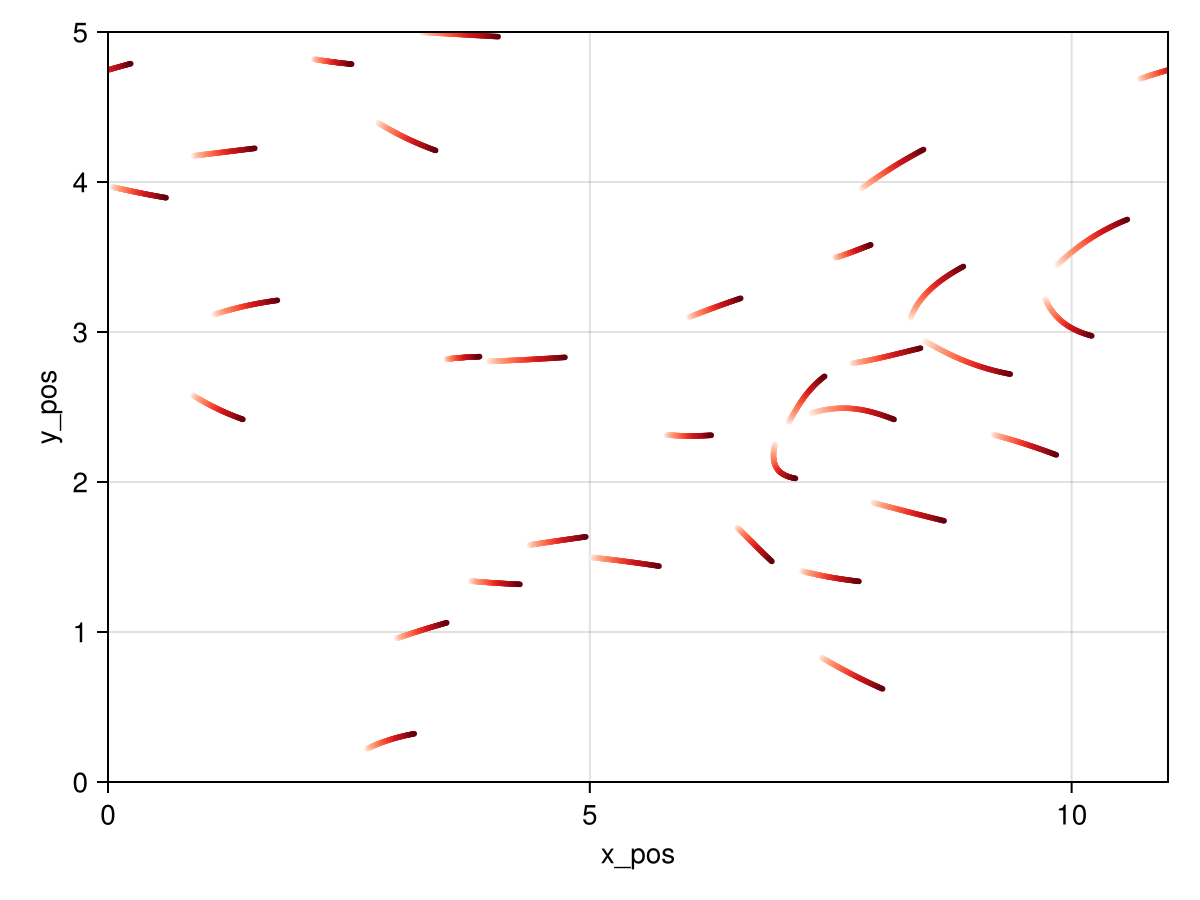
\includegraphics[width=\linewidth]{figures/Uniflowdflow_101.png}
        \caption{Unidirectional flow [start]}
    \end{subfigure}
    \begin{subfigure}{.49\textwidth}
        \centering
        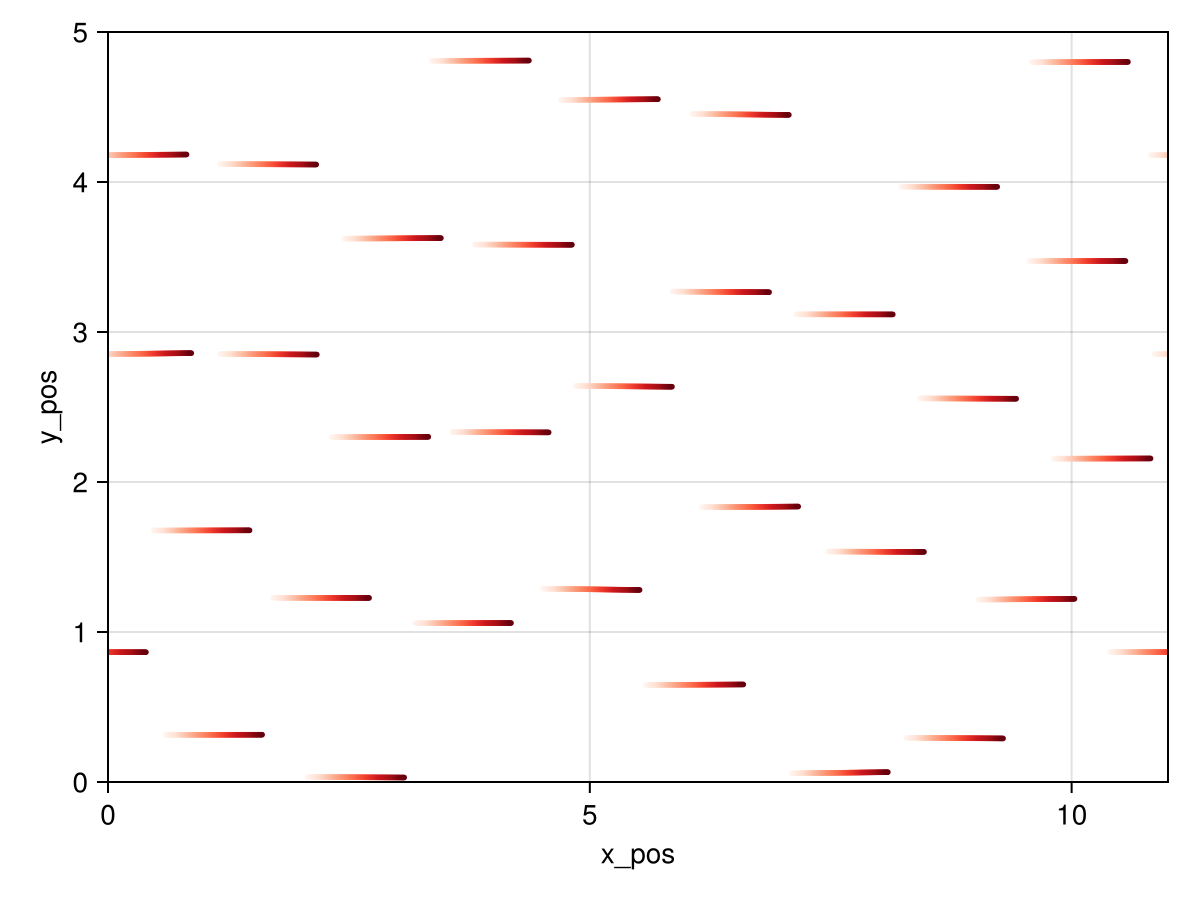
\includegraphics[width=\linewidth]{figures/Uniflowdflow_4000.png}
        \caption{Unidirectional flow [steady-state]}
    \end{subfigure}
    \caption{The progress of the simulation at (a) the start of the simulation and (b) after some time, reaching a steady state}
    \label{plot:uniflow_positions}
\end{figure}

\pagebreak
It can be observed from \autoref{plot:uniflow_positions} how the pedestrians start from a random arrangement and gradually reach a steady state by achieving their desired unidirectional motion.
\begin{figure}[H]
    \centering
    \begin{subfigure}{.49\textwidth}
        \centering
        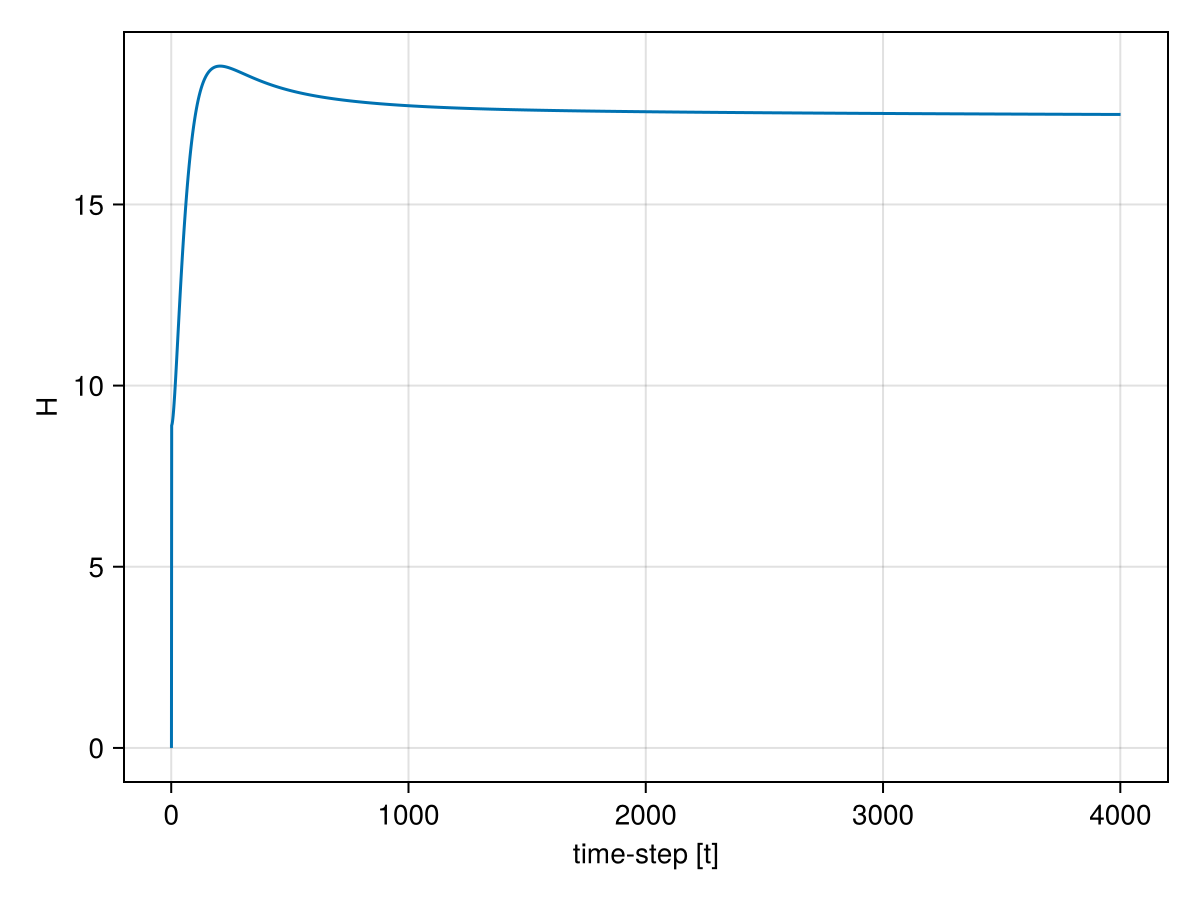
\includegraphics[width=\linewidth]{figures/H_Uniflow.png}
    \end{subfigure}
    \begin{subfigure}{.49\textwidth}
        \centering
        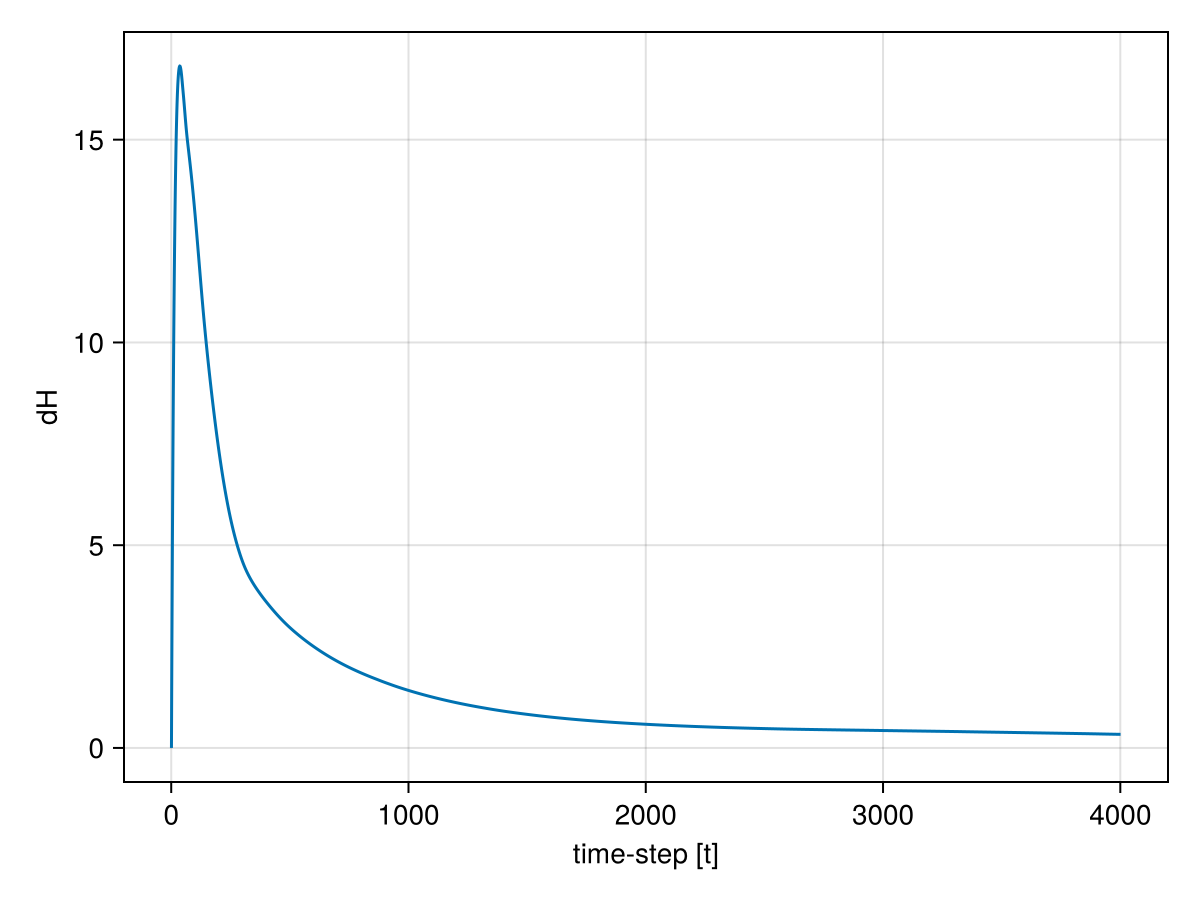
\includegraphics[width=\linewidth]{figures/dH_Uniflow.png}
    \end{subfigure}
    \caption{$H(z(t))$ and $\frac{d}{dt}H$ as the simulation progresses over time.}
    \label{plot:uniflow_hamiltonian}
\end{figure}

As demonstrated in \autoref{plot:uniflow_hamiltonian} the change in Hamiltonian with respect to time, $\frac{d}{dt}H(z(t))$ tends to zero as the system reaches its steady state. Using this solution of the uni-directional flow, we have generated a plot for the errors obtained from each numerical scheme in \autoref{plot:errors}. The plot \autoref{plot:scheme_error} shows the mean errors obtained for solving the model using a numerical scheme with fixed time-steps $\delta \text{t}$, whereas \autoref{plot:scheme_time} illustrates the computation time required to solve the model for fixed time-steps $\delta \text{t}$.

\begin{figure}[H]
    \centering
    \begin{subfigure}{.49\textwidth}
        \centering
        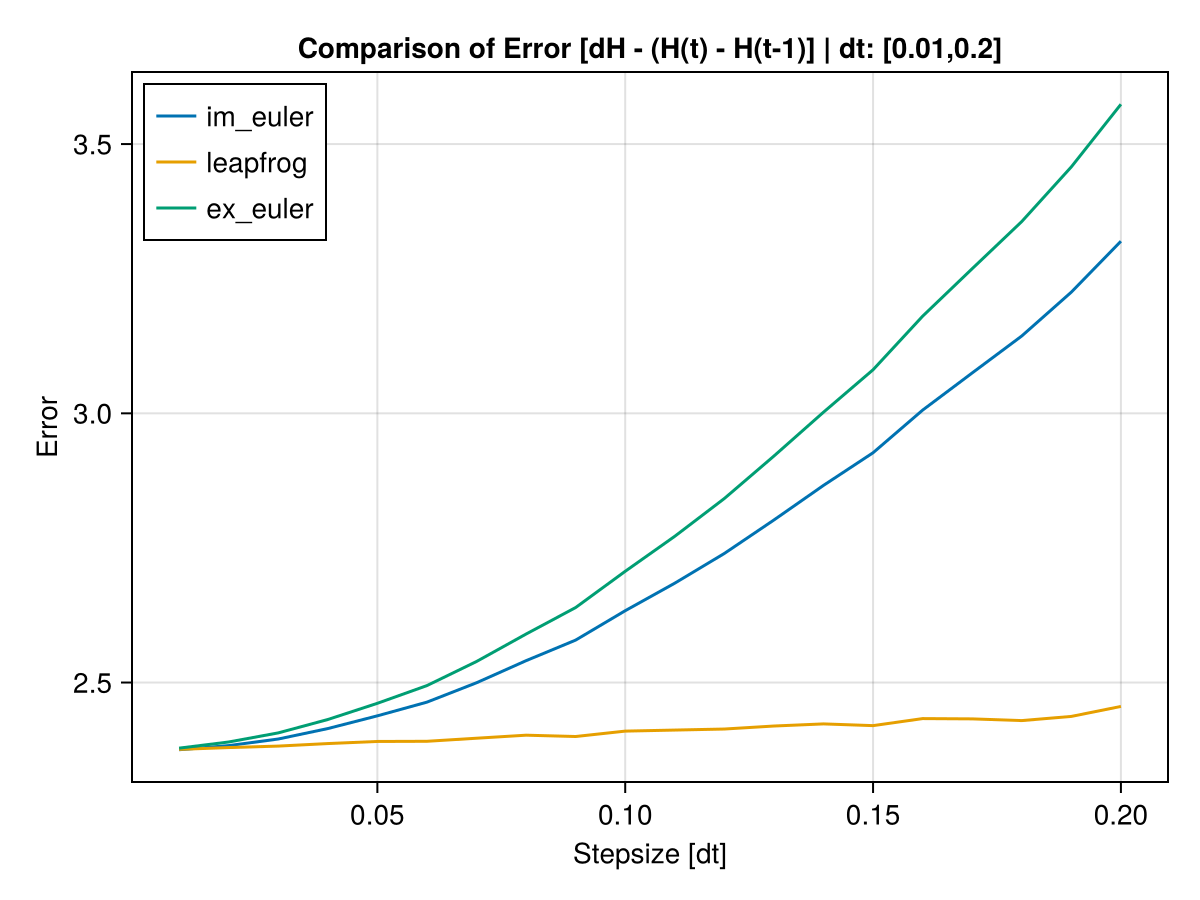
\includegraphics[width=\linewidth]{figures/manual_scheme_error1.png}
        \caption{Mean error of the schemes}
        \label{plot:scheme_error}
    \end{subfigure}
    \begin{subfigure}{.49\textwidth}
        \centering
        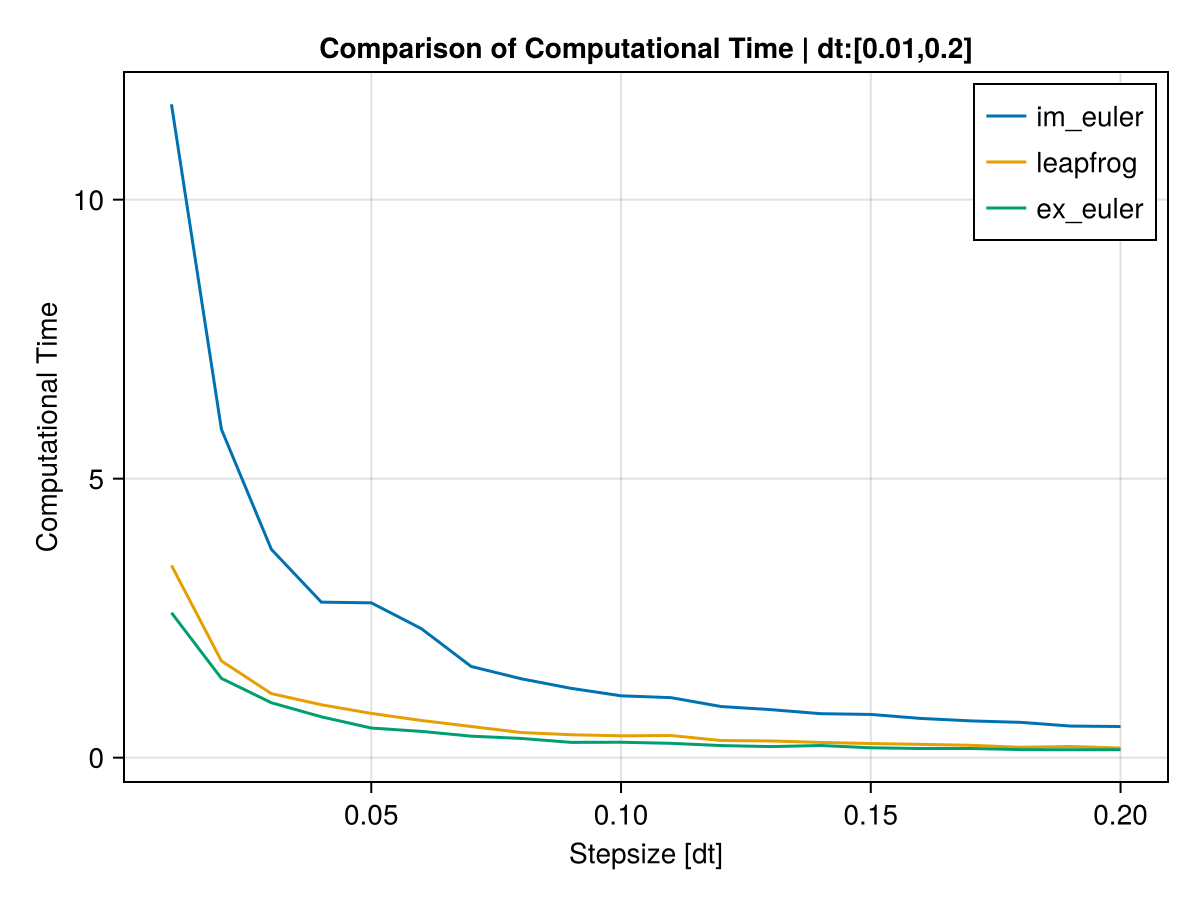
\includegraphics[width=\linewidth]{figures/time1.png}
        \caption{Computation time of the schemes}
        \label{plot:scheme_time}
    \end{subfigure}
    \caption{Comparison of numerical schemes in terms error and computation time}
    \label{plot:errors}
\end{figure}

As one would expect the errors do increase when the $\delta \text{t}$ increases, however the stark contrast between the minute numerical errors of leapfrog scheme to others clearly shows the benefit of using symplectic schemes for solving Hamiltonian systems. The computation time of leapfrog here is similar to that of explicit Euler. Implicit Euler, on the other hand, yields results that are only slightly better than its explicit counterpart regarding errors. Due to its implicit nature, the implicit Euler also requires extra steps to numerically solve equations resulting it to be the most computationally expensive compared to the other two.

With these results in mind, we conclude this section with leapfrog as our choice to be used for all deterministic dynamical models for our simulations in the coming section.

\pagebreak
\section{Simulation and Observations}
In this section we make use of our model by simulating it for various cases. First we will demonstrate some basic dynamics based on the impact of dissipation $\lambda$, desired velocities $u_i$, and interaction $A$. Next we will focus on collective behavior, and present formations such as lane and stripe formations for counter and cross flows respectively. Some insights are provided on the relationship between the parameters, Hamiltonian, and the collective behavior.

The model parameters defined for the simulation are the same as defined in \autoref{code:model_init}. Any changes made would be mentioned within their respective cases. For reproducibility and comparison, each simulation starts with the same arrangement of pedestrians on the xy-plane as shown in 
\begin{figure}[H]
    \centering
    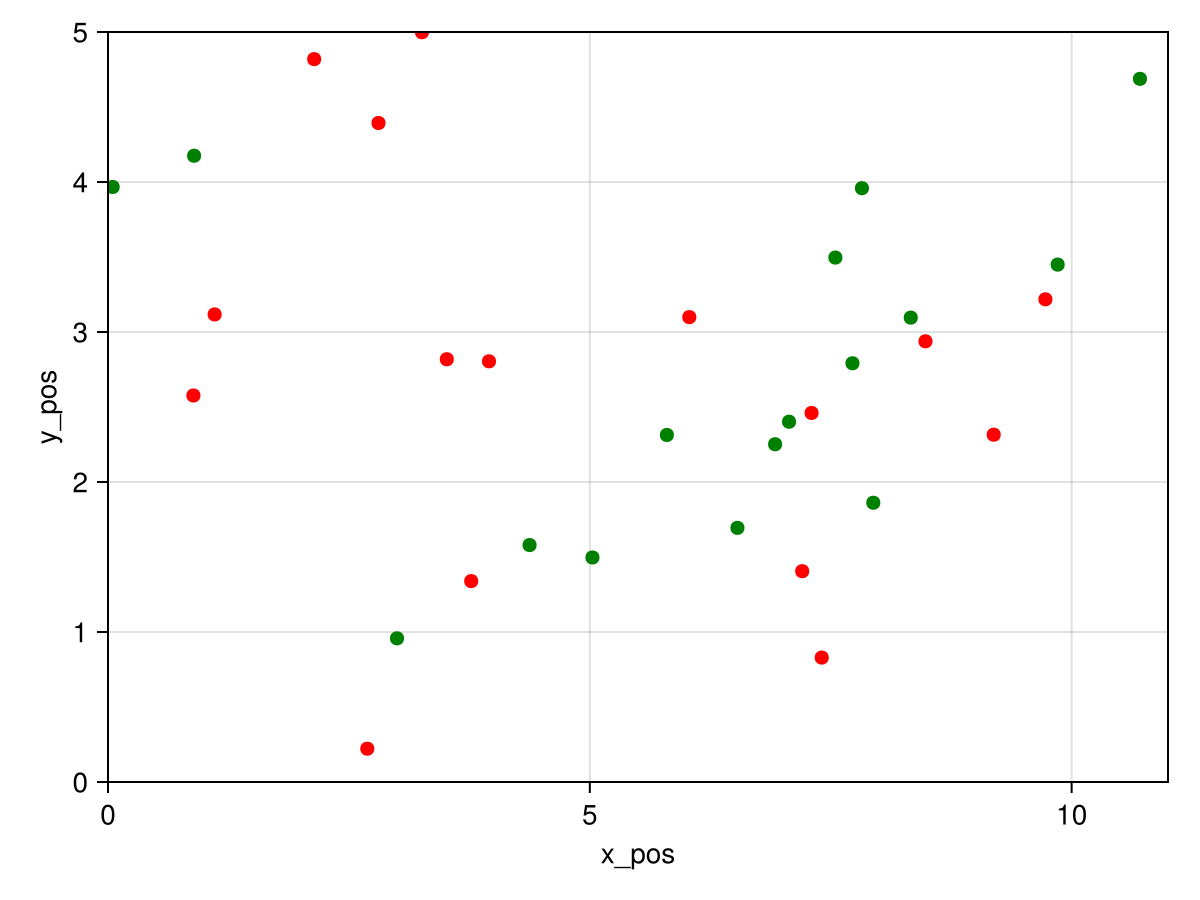
\includegraphics[width=0.55\textwidth]{figures/start_pos.png}
    \caption{Starting positions of pedestrians.}
    \label{plot:starting_pos}
\end{figure}
The color in \autoref{plot:starting_pos} distinguishes between the desired speeds of the pedestrians, which is only relevant for flows that are not unidirectional, as will be shown in \autoref{section:collective}. In the cases of unidirectional flow or where the direction is irrelevant, the color for all is the same.

\subsection{Basic Dynamics}
This section serves to illustrate how the changes in the parameters affect the dynamics of the model, although none of the dynamics presented in the model are realistic, the diagrams provide a way to think about the dynamics of the model based on the changes in the parameter.
\pagebreak
\begin{itemize}
    \item \textbf{No desired velocity ($u_i = \begin{bmatrix} 0 & 0 \end{bmatrix}$) with dissipation ($\lambda > 0$):}
\begin{figure}[H]
    \centering
    \begin{subfigure}{\textwidth}
        \centering
        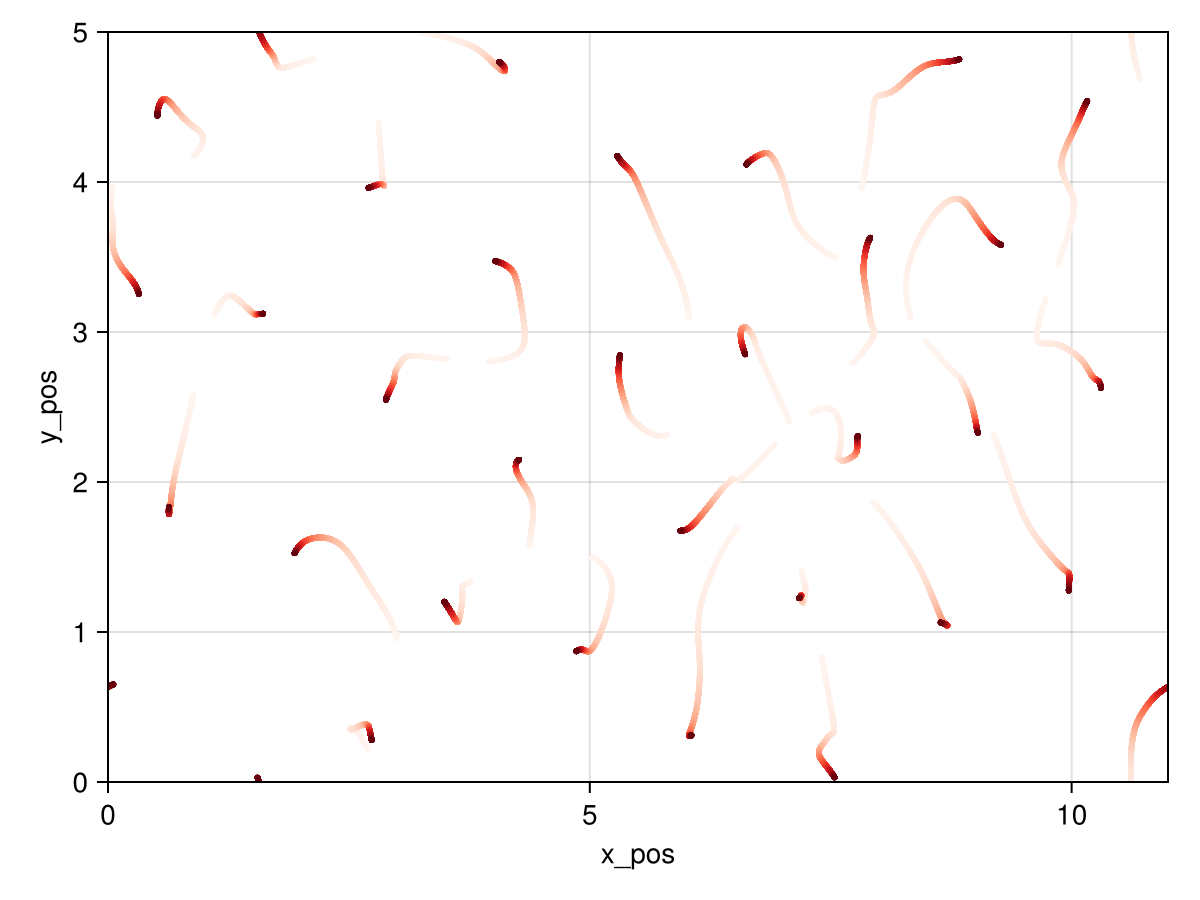
\includegraphics[width=0.6\linewidth]{figures/crystallizationdflow_4001.png}
        \caption{Pedestrian trajectories}
        \label{plot:crys_traj}
    \end{subfigure}
    \begin{subfigure}{.40\textwidth}
        \centering
        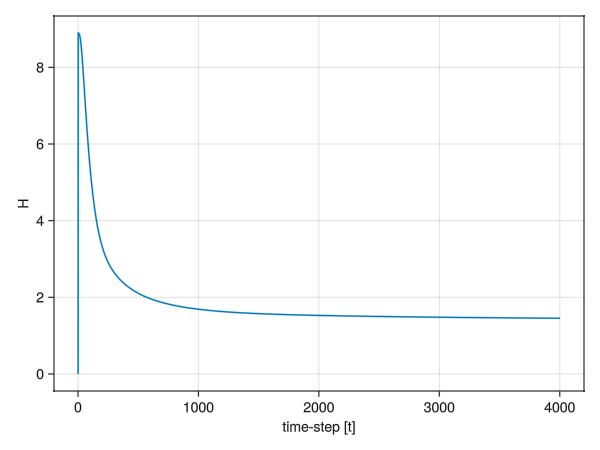
\includegraphics[width=\linewidth]{figures/H_crystallization.png}
        \caption{Hamiltonian $(H)$}
        \label{plot:crys_h}
    \end{subfigure}
    \begin{subfigure}{.40\textwidth}
        \centering
        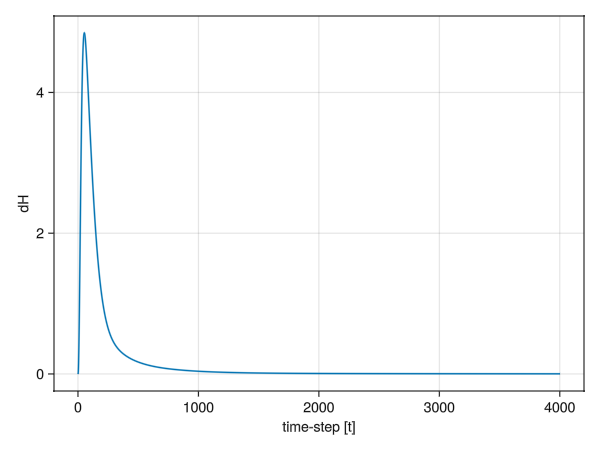
\includegraphics[width=\linewidth]{figures/dH_crystallization.png}
        \caption{Time derivative of Hamiltonian $\frac{d}{dt}H$}
        \label{plot:crys_dh}
    \end{subfigure}
    \caption{Crystallization of pedestrians due to no input $u_i = 0$ and allowing the system to dissipate energy}
    \label{plot:crys}
\end{figure}
Allowing the system to dissipate $\lambda > 0$ while simultaneously the pedestrians have no desired velocity \autoref{plot:crys}, essentially creates a system with an active output port, but no input. The results are as expected, the system keeps losing energy leading the pedestrians to crystallize over time. The Hamiltonian, which is a representation of the total energy of the system relaxes towards lower energy levels asymptotically reaching zero.
\pagebreak
\item \textbf{No dissipation ($\lambda = 0$)}
\begin{figure}[H]
    \centering
    \begin{subfigure}{\textwidth}
        \centering
        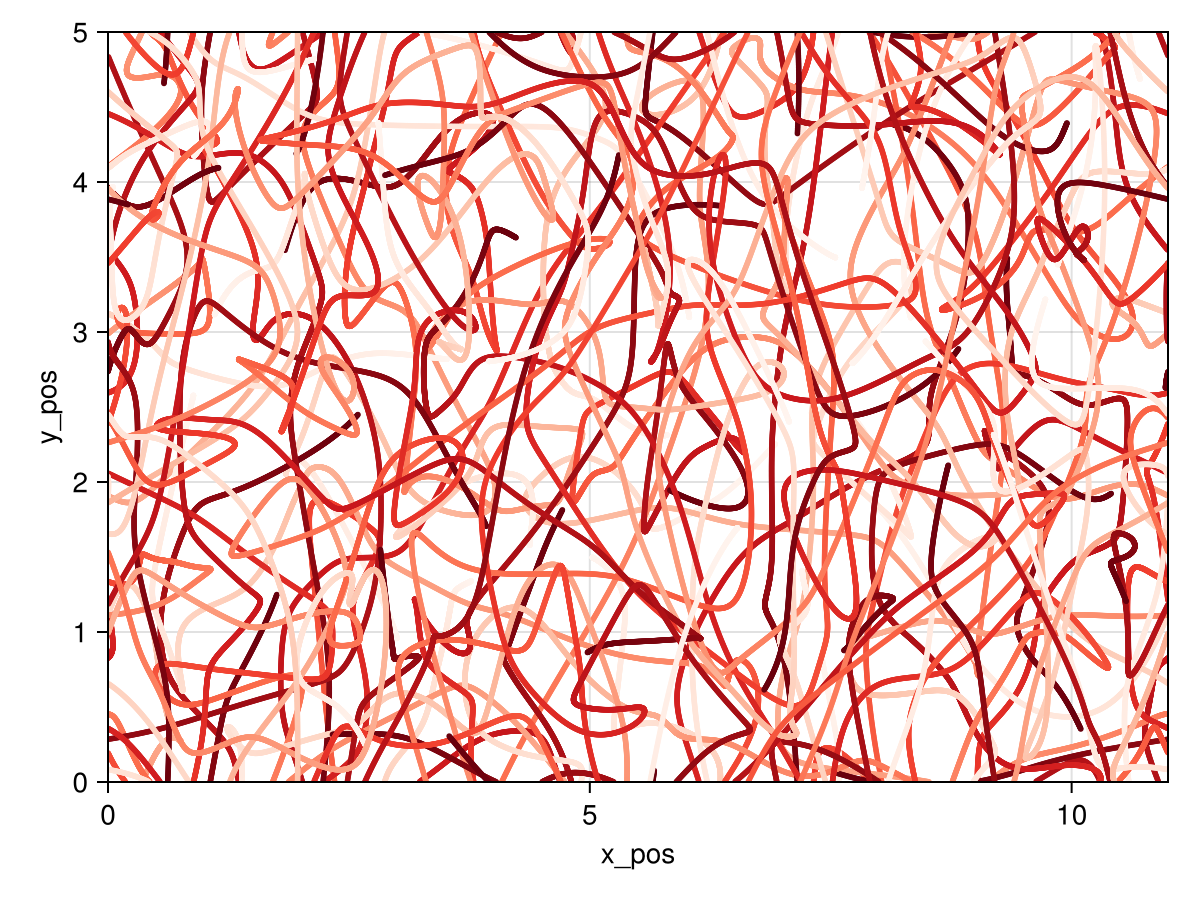
\includegraphics[width=0.6\linewidth]{figures/no_dissipationdflow_4001.png}
        \caption{Pedestrian trajectories}
        \label{plot:nodisp_traj}
    \end{subfigure}
    \begin{subfigure}{.40\textwidth}
        \centering
        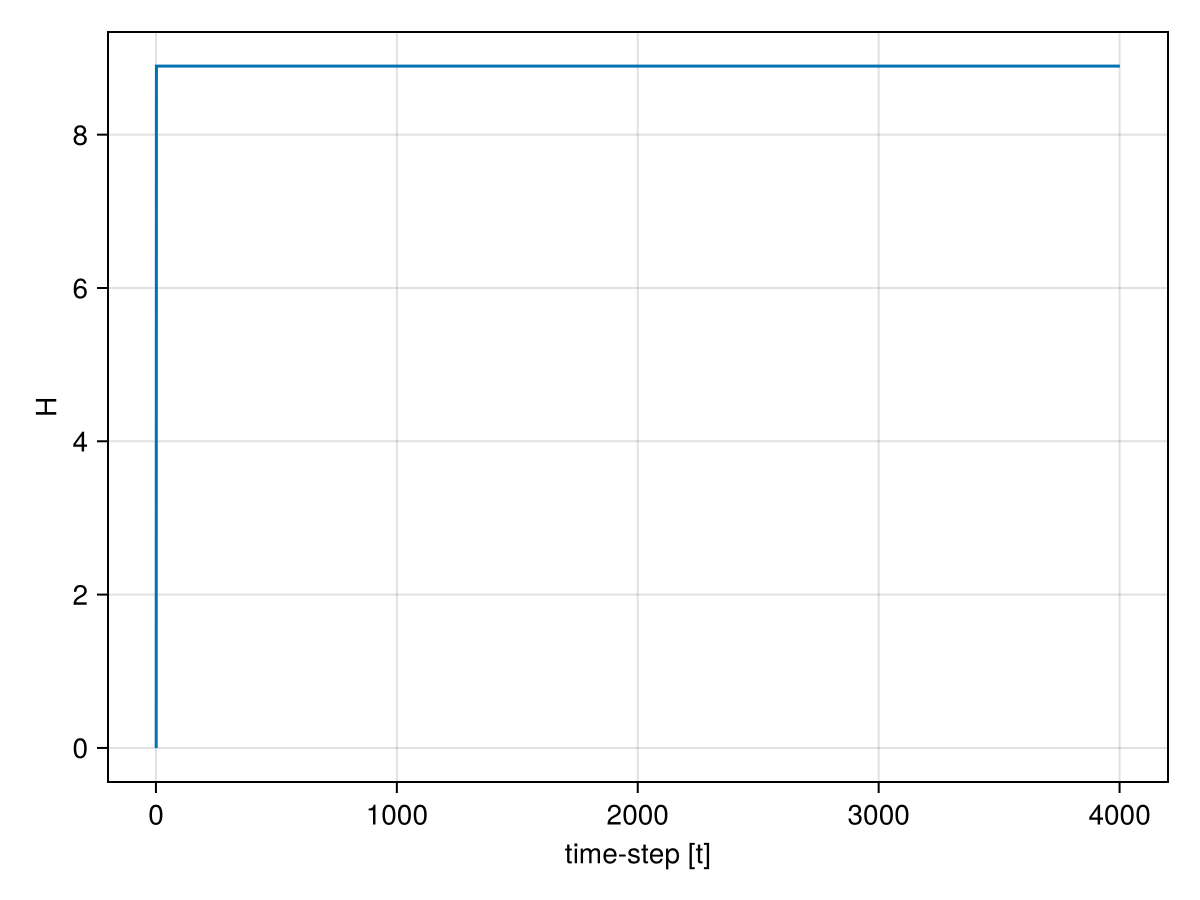
\includegraphics[width=\linewidth]{figures/H_no_dissipation.png}
        \caption{Hamiltonian $(H)$}
        \label{plot:nodisp_h}
    \end{subfigure}
    \begin{subfigure}{.40\textwidth}
        \centering
        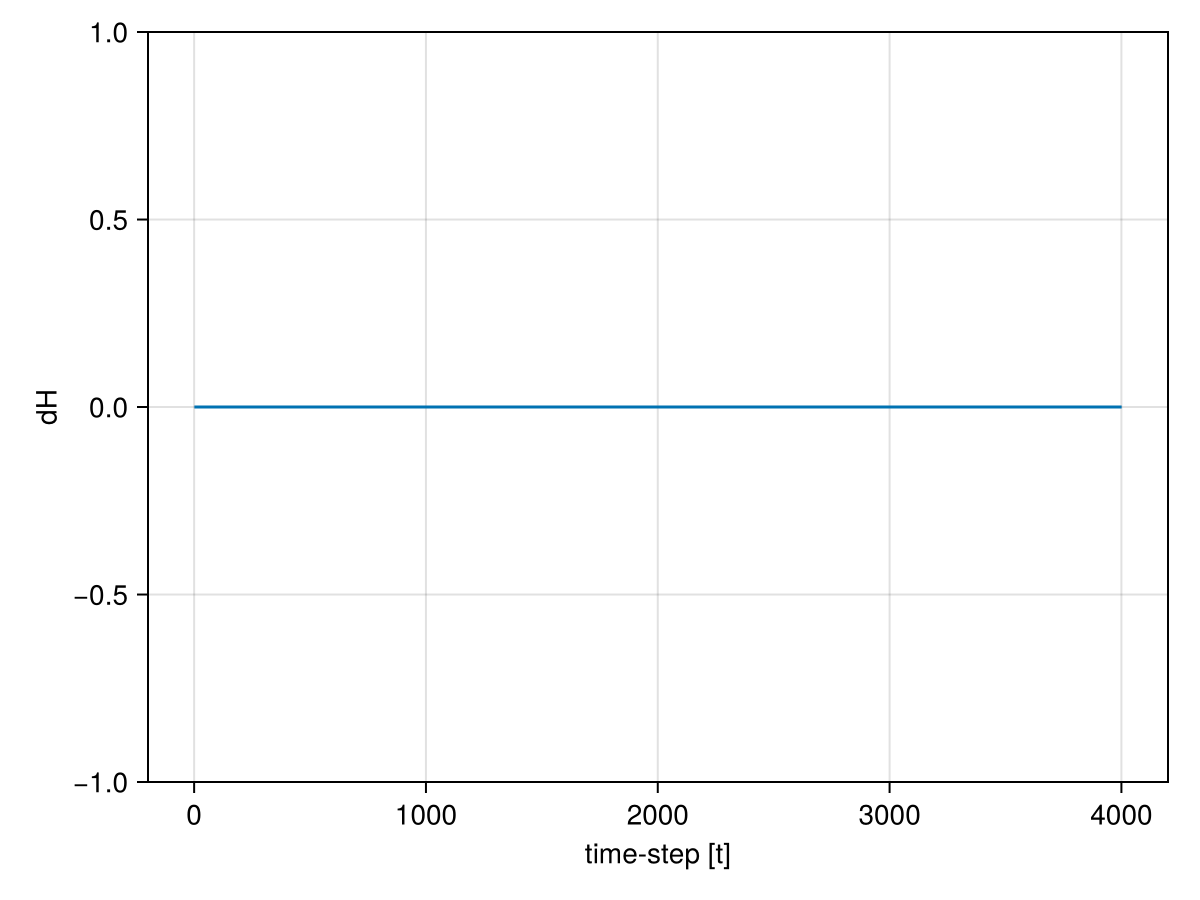
\includegraphics[width=\linewidth]{figures/dH_no_dissipation.png}
        \caption{Time derivative of Hamiltonian $\frac{d}{dt}H$}
        \label{plot:nodisp_dh}
    \end{subfigure}
    \caption{Trajectories of pedestrians in a non-dissipative system ($\lambda = 0$)}
    \label{plot:nodisp}
\end{figure}

Given the dynamics formulated in \autoref{eq:ph_model}, it can be clearly seen that $\lambda$ exists both as a coefficient of the input port $\tilde u$ as well as in the output port $y$. Thus setting $\lambda = 0$ clearly suggests that the resulting system has no dissipation as well as no energy feed. Consequently, the pedestrians move with no direction \autoref{plot:nodisp_traj} regardless of the fact the desired velocity is provided.

The resulting system is a conservative Hamiltonian system, as by consequence the dissipative term $R$ also vanishes. This can be clearly observed as the Hamiltonian remains constant over time. It is to be noted that the immediate jump of the Hamiltonian in \autoref{plot:nodisp_h} is simply because the Hamiltonian was initialized to zero (\autoref{code:model_init}) before the start of the simulation
\pagebreak
\item \textbf{No pedestrian interaction ($A = 0$) with $u_i = \begin{bmatrix} 1 & 0 \end{bmatrix}$}
\begin{figure}[H]
    \centering
    \begin{subfigure}{\textwidth}
        \centering
        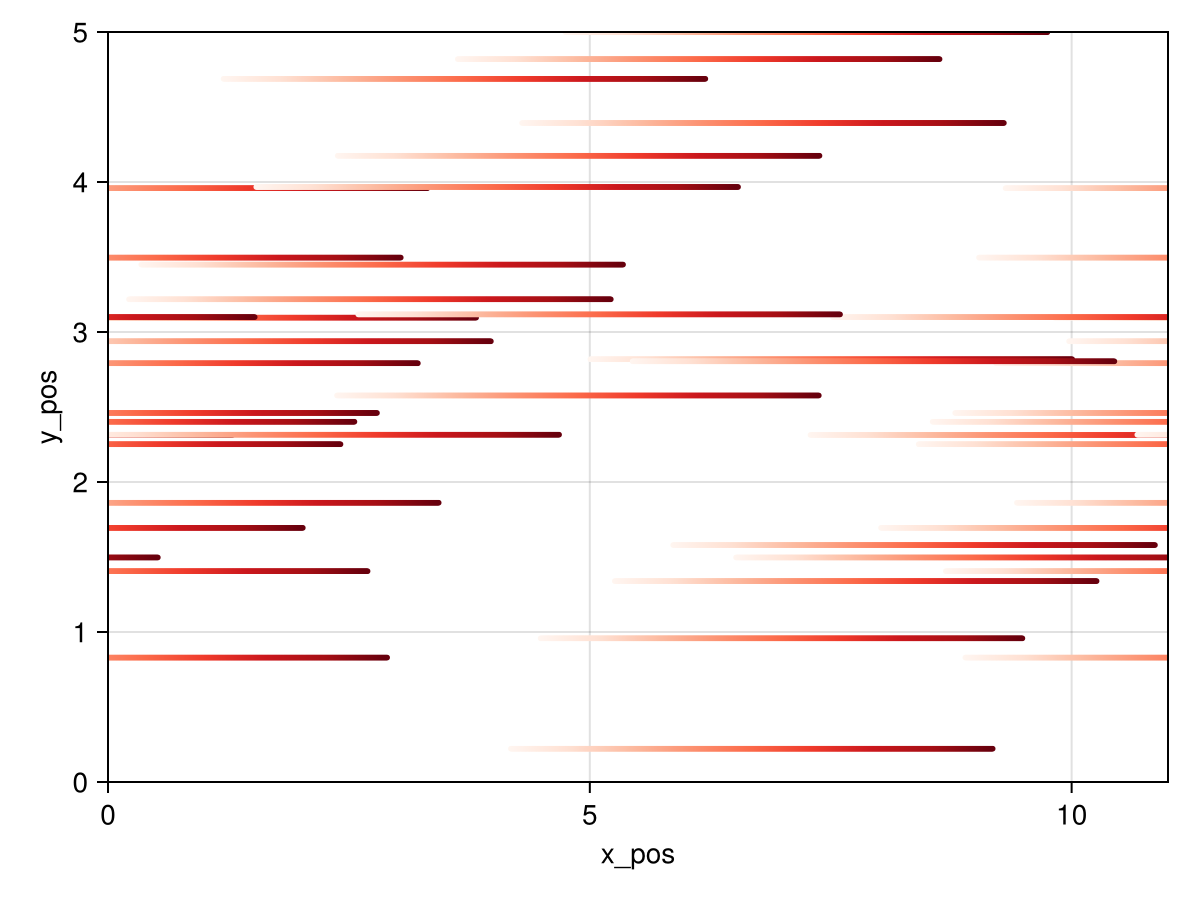
\includegraphics[width=0.6\linewidth]{figures/no_interactiondflow_4000.png}
        \caption{Pedestrian trajectories}
        \label{plot:nointeraction_traj}
    \end{subfigure}
    \begin{subfigure}{.40\textwidth}
        \centering
        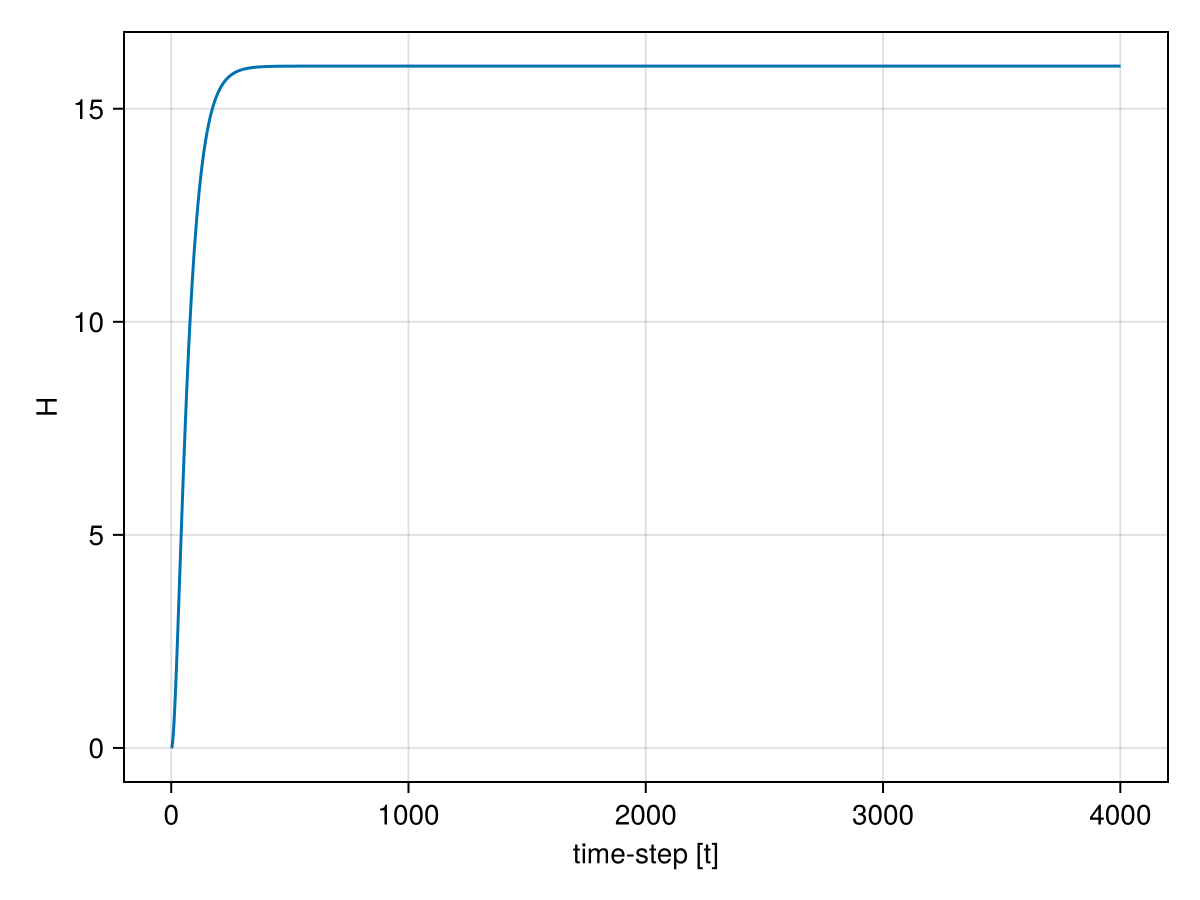
\includegraphics[width=\linewidth]{figures/H_no_interaction.png}
        \caption{Hamiltonian $(H)$}
        \label{plot:nointeraction_h}
    \end{subfigure}
    \begin{subfigure}{.40\textwidth}
        \centering
        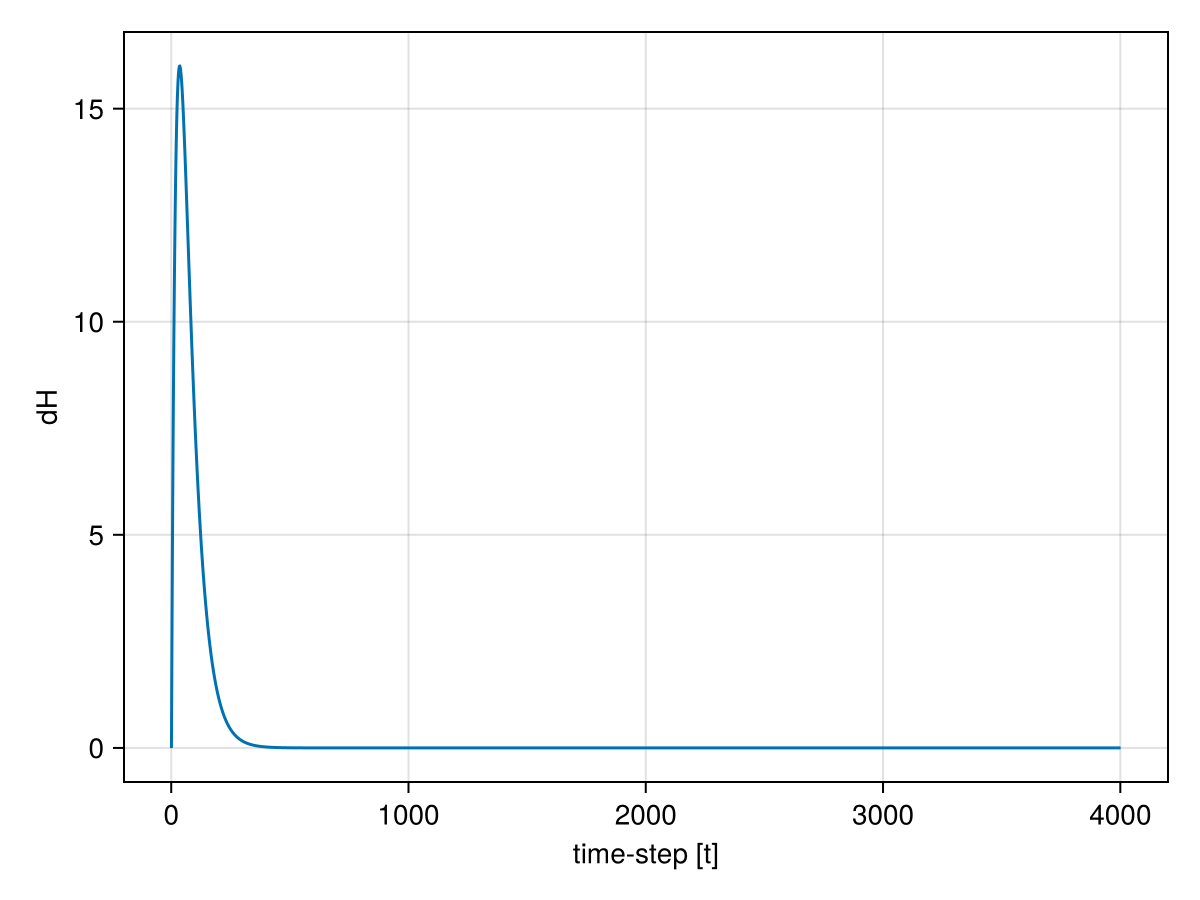
\includegraphics[width=\linewidth]{figures/dH_no_interaction.png}
        \caption{Time derivative of Hamiltonian $\frac{d}{dt}H$}
        \label{plot:nointeraction_dh}
    \end{subfigure}
    \caption{Trajectories of pedestrians with no interaction with other pedestrian ($ A = 0 $) and desired velocities $u_i = \begin{bmatrix}1 & 0\end{bmatrix} $}
    \label{plot:nointeraction}
\end{figure}

By setting $A = 0$, the pedestrians in the system move with no interactivity with other pedestrians in the system. Essentially, every pedestrian simply move with their desired velocities as soon the simulation begins \autoref{plot:nointeraction}. Because this parameter directly effects the interaction potential $U(x)$ in \autoref{eq:def_potU}, it can be clearly observed that the motion of the pedestrian is independent of their distance to each other, in other words they move with no concern to how close or far they are from other pedestrians.

Given the lack of interaction, the pedestrians move with their desired velocities, thus in the long run, the Hamiltonian need not be dependent on time, but instead the desired velocities of the pedestrians -- mathematically $p_i = u_i$. One can also obtain this long term value of the Hamiltonian $H^*(u)$ by setting $A = 0$ (as it is for this case) in \autoref{eq:Hamiltonian} leading to 
\begin{align}
    H(z(t)) = \dfrac{1}{2}||p(t)||^2 \rightarrow H^*(u) = \dfrac{1}{2}||u||^2
    \label{eq:Hstar}
\end{align}

This expression for the long term Hamiltonian $H^*(u)$ is a function of the desired velocities $u_i$. As $u_i$ is set by the user, one easily evaluate this value. Even with potential interaction allowed in the system dynamics, the expression serves as a representation of what the system as a whole is trying to attain. Ideally, every pedestrian wants to achieve the desired velocity $u_i$, and the system as a whole wants to achieve the energy $H^*$. 
\end{itemize}



\subsection{Collective Dynamics}
\label{section:collective}

In this section however, we will witness collective phenomenon based on the desired speeds and relaxation (or dissipation) parameter $\lambda$. The pedestrians will start from the same random positions generated in \autoref{plot:starting_pos}, but with different desired speeds $u_i$. This disordered arrangement goes through a phase transition and form ordered patterns, such as lane formation and stripe formation. We will notice how a sufficient $\lambda$ is needed to achieve these phase transitions. Furthermore, we will see how $H^*(u)$ from \autoref{eq:Hstar} ties in as an order parameter to identify collective behaviors.
\begin{itemize}
    \item \textbf{Lane Formation for counter flow with $\lambda = 2$}
    \begin{figure}[H]
        \centering
        \begin{subfigure}{\textwidth}
            \centering
            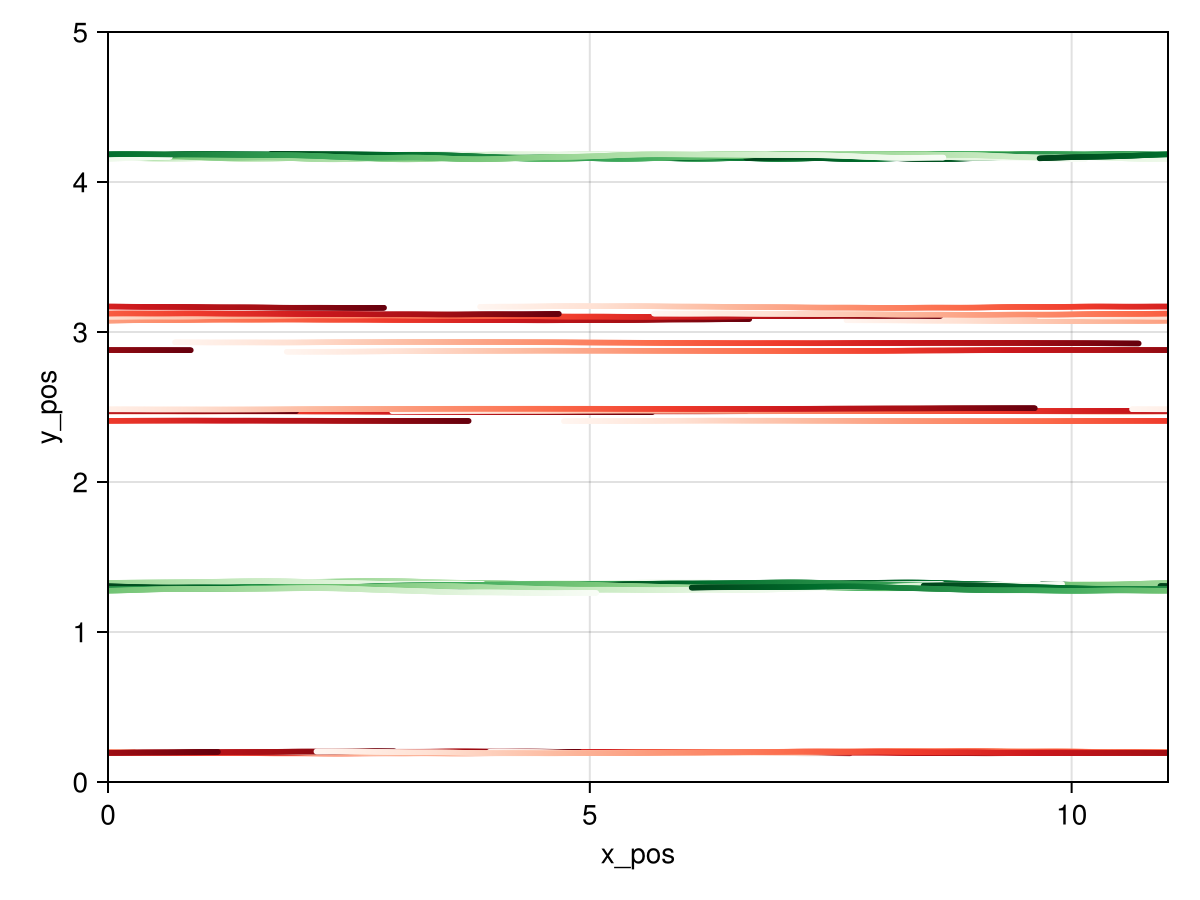
\includegraphics[width=0.6\linewidth]{figures/s0_fbh_1noflow_10000.png}
            \caption{Pedestrian trajectories}
            \label{plot:counter_traj}
        \end{subfigure}
        \begin{subfigure}{.40\textwidth}
            \centering
            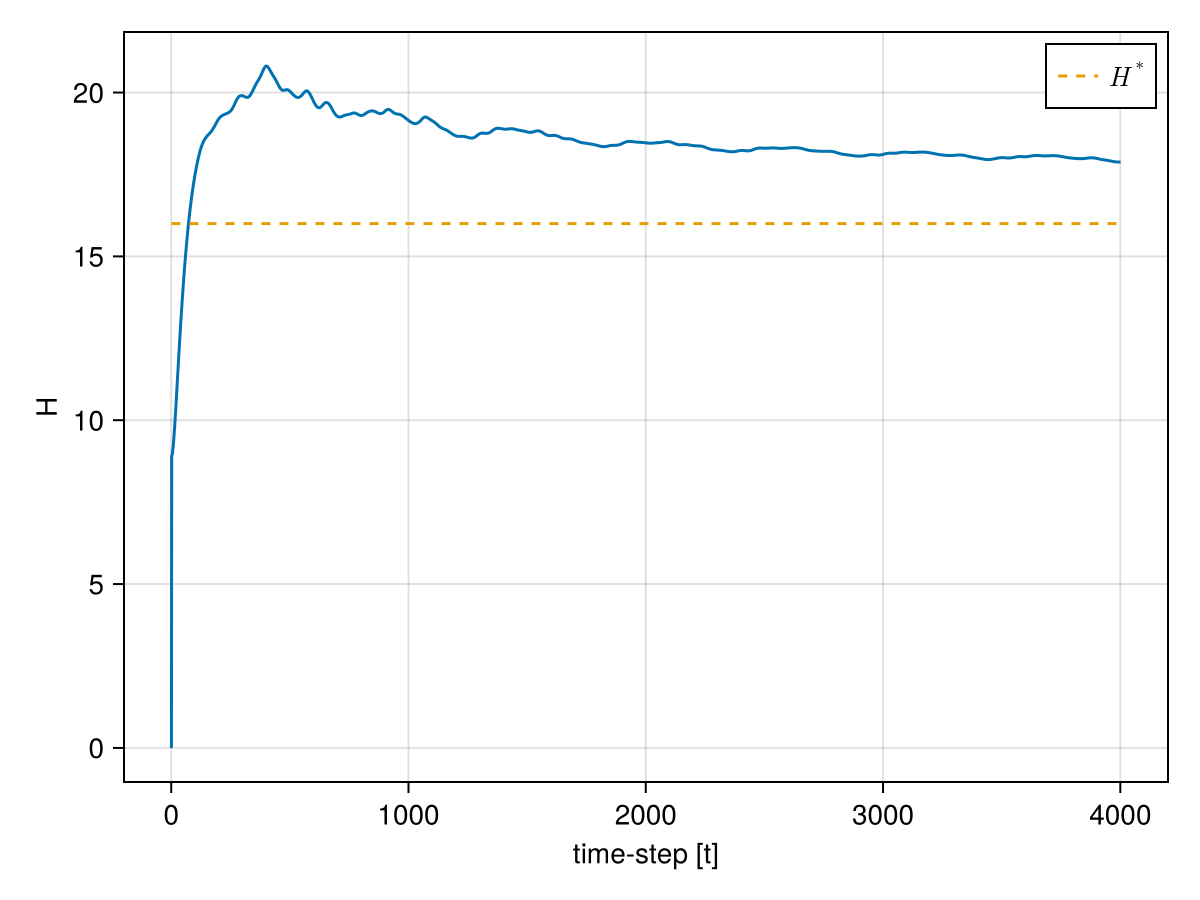
\includegraphics[width=\linewidth]{figures/H_counter.png}
            \caption{Hamiltonian $(H)$}
            \label{plot:counter_h}
        \end{subfigure}
        \begin{subfigure}{.40\textwidth}
            \centering
            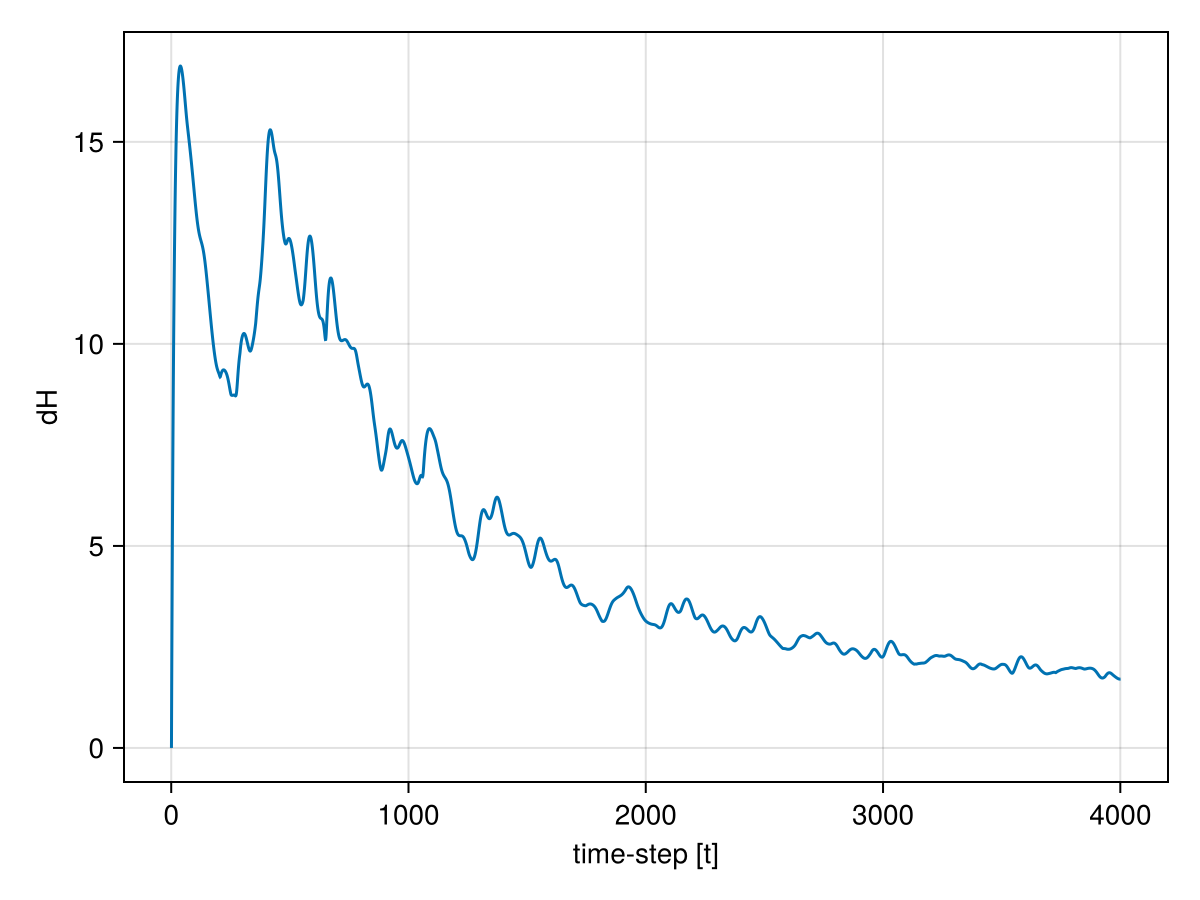
\includegraphics[width=\linewidth]{figures/dH_counter.png}
            \caption{Time derivative of Hamiltonian $\frac{d}{dt}H$}
            \label{plot:counter_dh}
        \end{subfigure}
        \caption{Emergence of lane formation as pedestrians move in counter flow}
        \label{plot:counter}
    \end{figure}
Starting from a random assortment of pedestrians as shown in \autoref{plot:starting_pos}, with predefined desired velocities $u_i = \begin{bmatrix} 1 & 0 \end{bmatrix}$ for half of the pedestrians (Red), and $u_i = \begin{bmatrix} -1 & 0 \end{bmatrix}$ for the other half (Green), as shown in \autoref{code:agent_init}. As the time progresses, the pedestrians form lanes. From a point of view of energy in the system, the pedestrians self-organize themselves in a manner such that the Hamiltonian reaches a steady state and remains above $H^*$, while $\frac{d}{dt}H$ reaches zero. 

    \item \textbf{Gridlock for counter flow with $\lambda = 0.2$}
    \begin{figure}[H]
        \centering
        \begin{subfigure}{\textwidth}
            \centering
            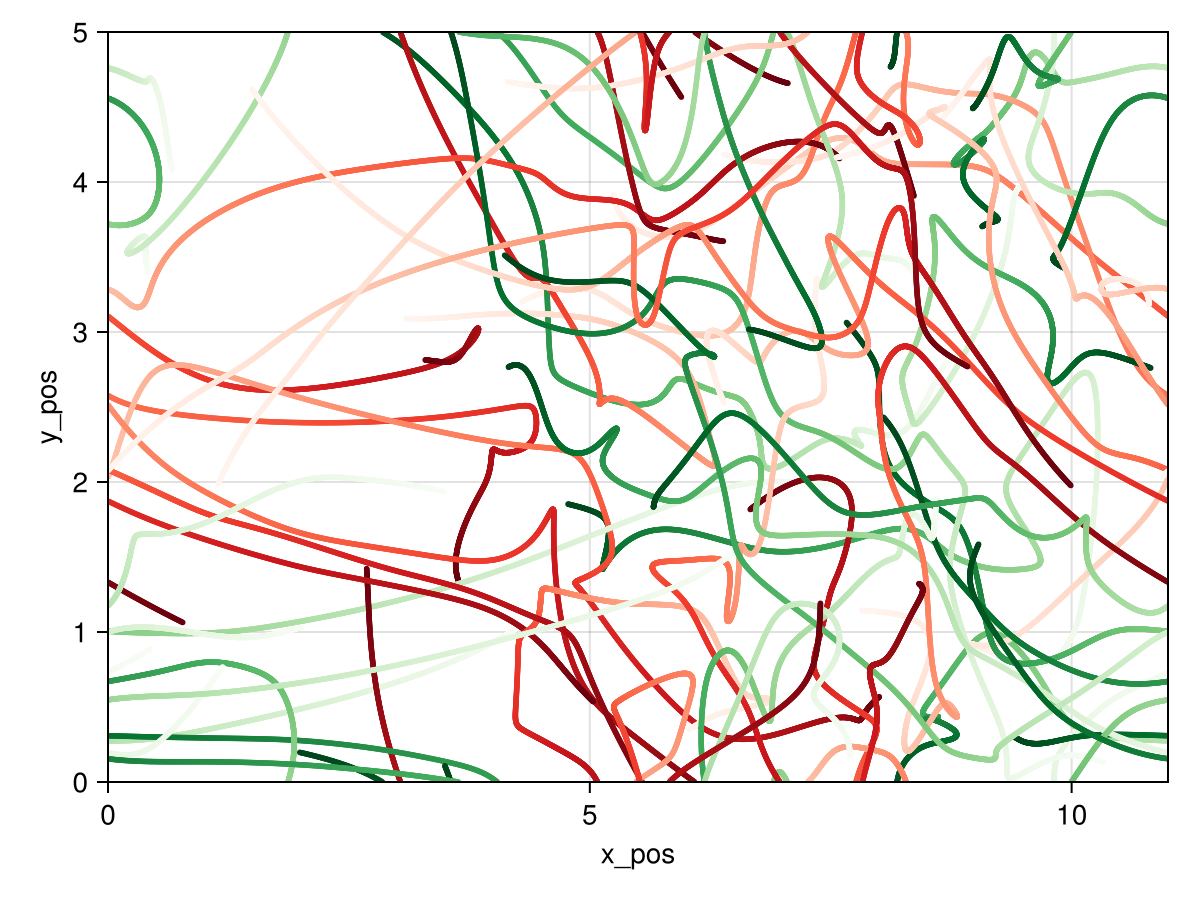
\includegraphics[width=0.6\linewidth]{figures/counter_gridlockdflow_4000.png}
            \caption{Pedestrian trajectories}
            \label{plot:countergridlock_traj}
        \end{subfigure}
        \begin{subfigure}{.40\textwidth}
            \centering
            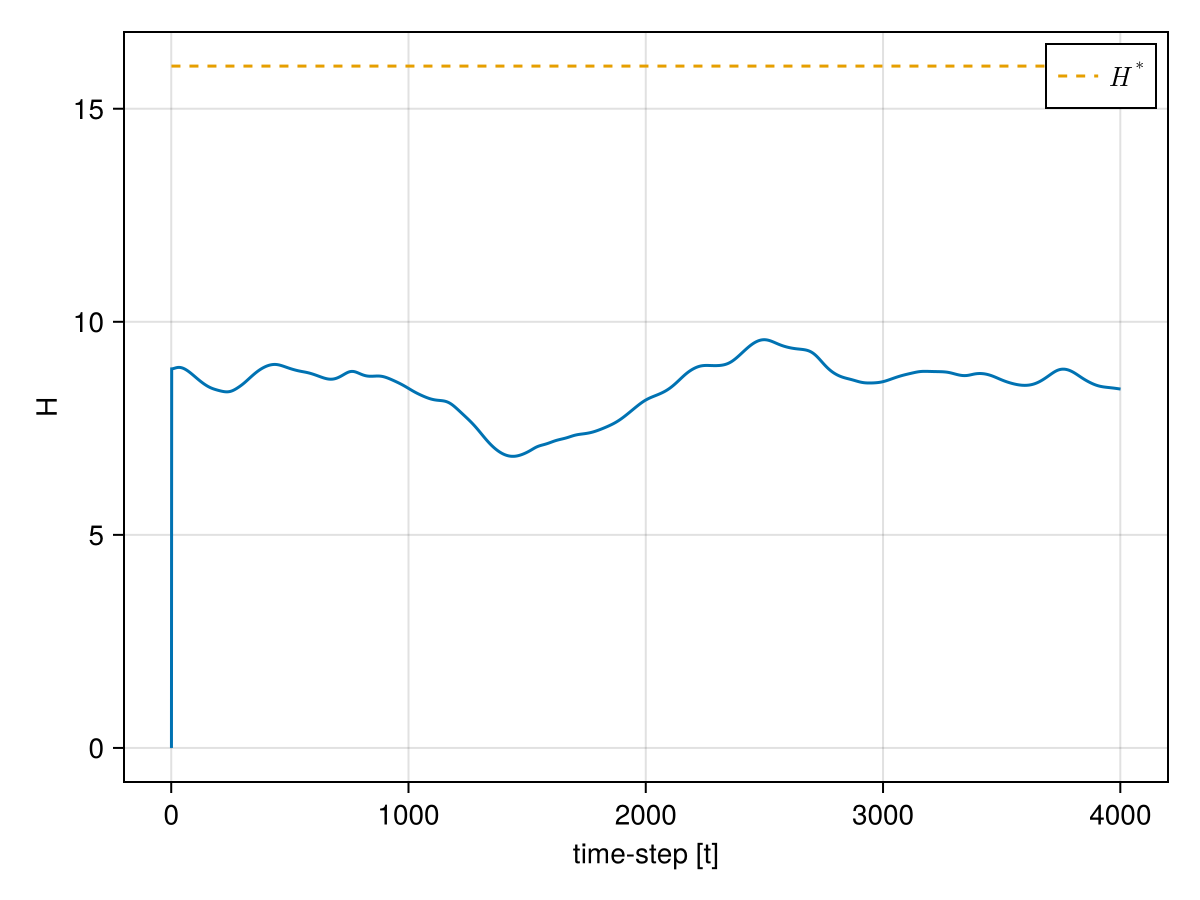
\includegraphics[width=\linewidth]{figures/H_counter_gridlock.png}
            \caption{Hamiltonian $(H)$}
            \label{plot:countergridlock_h}
        \end{subfigure}
        \begin{subfigure}{.40\textwidth}
            \centering
            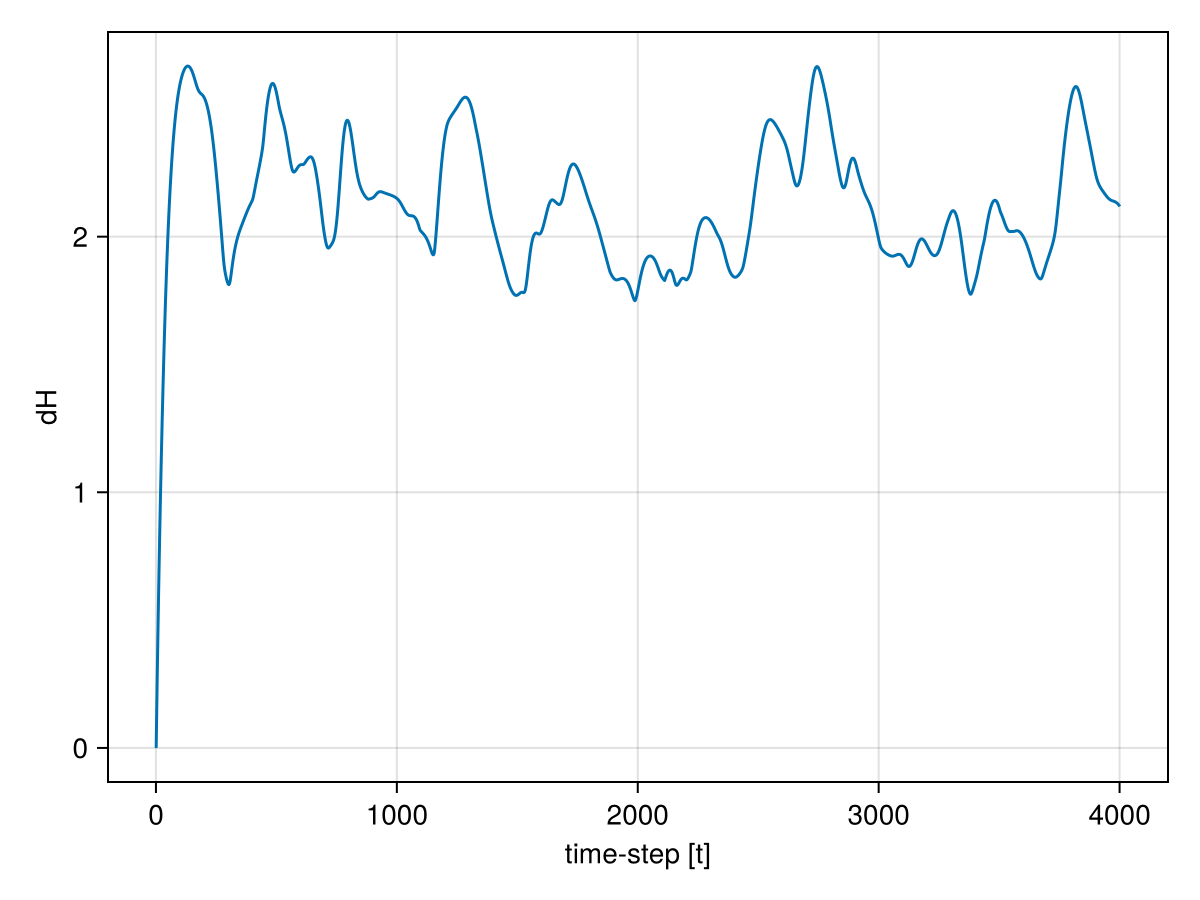
\includegraphics[width=\linewidth]{figures/dH_counter_gridlock.png}
            \caption{Time derivative of Hamiltonian $\frac{d}{dt}H$}
            \label{plot:countergridlock_dh}
        \end{subfigure}
        \caption{Gridlock for counter flow}
        \label{plot:countergridlock}
    \end{figure}
With the same parameters as the previous case, with the only difference being that $\lambda$ is not sufficiently high, it can be observed that no lane formation occurs. The system neither gains nor dissipates enough energy, resulting in pedestrians behaving similarly to the trajectories presented in \autoref{plot:nodisp}, leading to gridlocks. The Hamiltonian erratically fluctuates over time and remains below $H^*$.

Here the significance of $\lambda$ is apparent, as this parameter balances the conservation of energy enforced by the skew-symmetry with the flow of energy through dissipation and feed permitted by the ports.
\pagebreak
    \item \textbf{Stripe Formation for cross flow with $\lambda = 2$}
    \begin{figure}[H]
        \centering
        \begin{subfigure}{\textwidth}
            \centering
            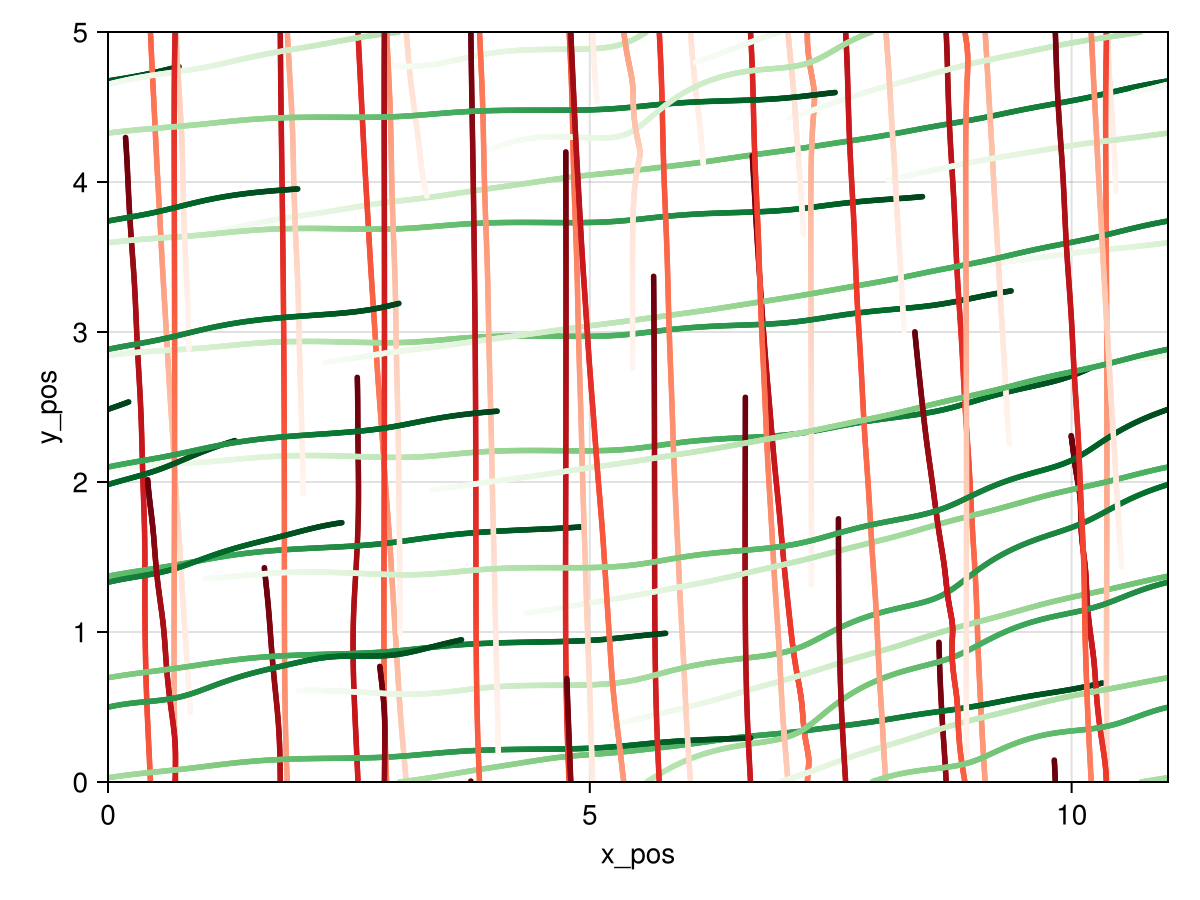
\includegraphics[width=0.6\linewidth]{figures/crossleapflow_10000.png}
            \caption{Pedestrian trajectories}
            \label{plot:cross2_traj}
        \end{subfigure}
        \begin{subfigure}{.40\textwidth}
            \centering
            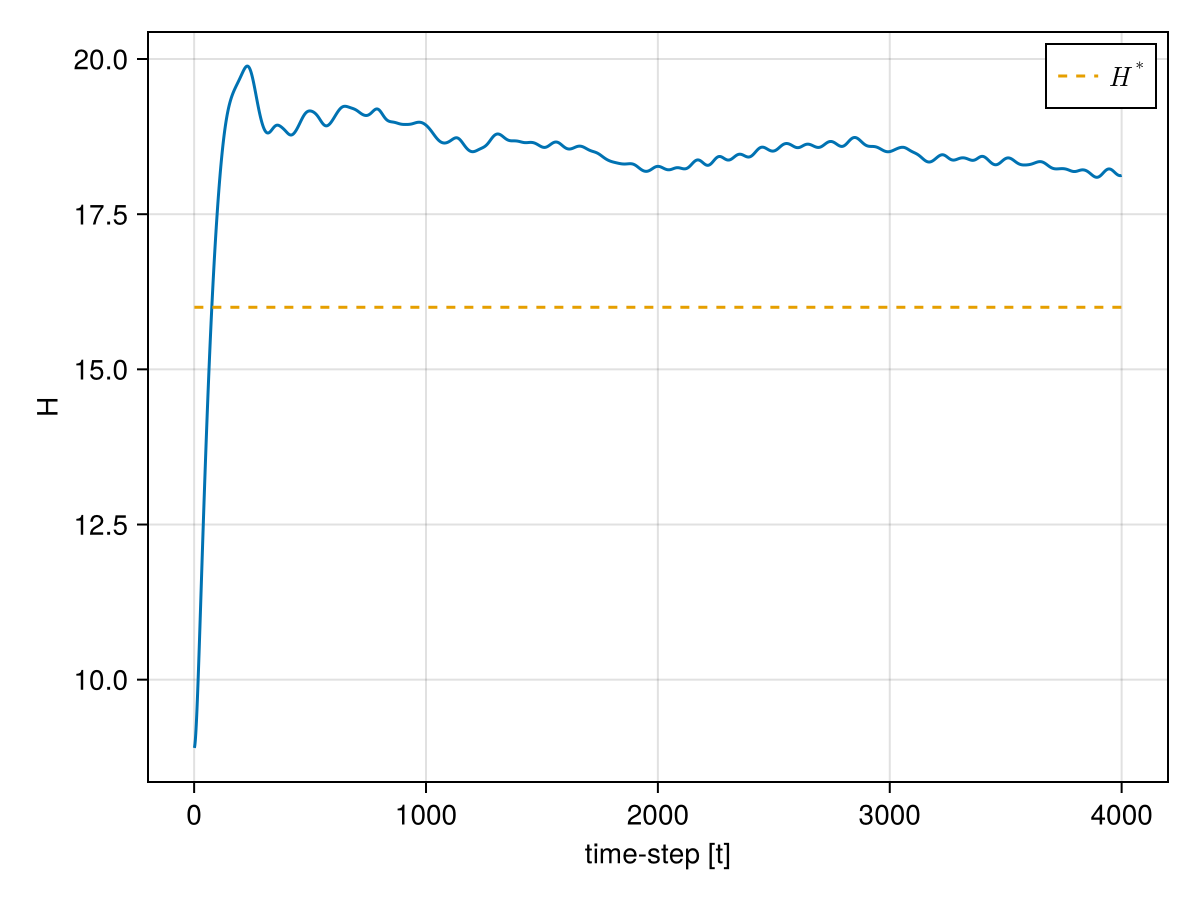
\includegraphics[width=\linewidth]{figures/H_cross2.png}
            \caption{Hamiltonian $(H)$}
            \label{plot:cross2_h}
        \end{subfigure}
        \begin{subfigure}{.40\textwidth}
            \centering
            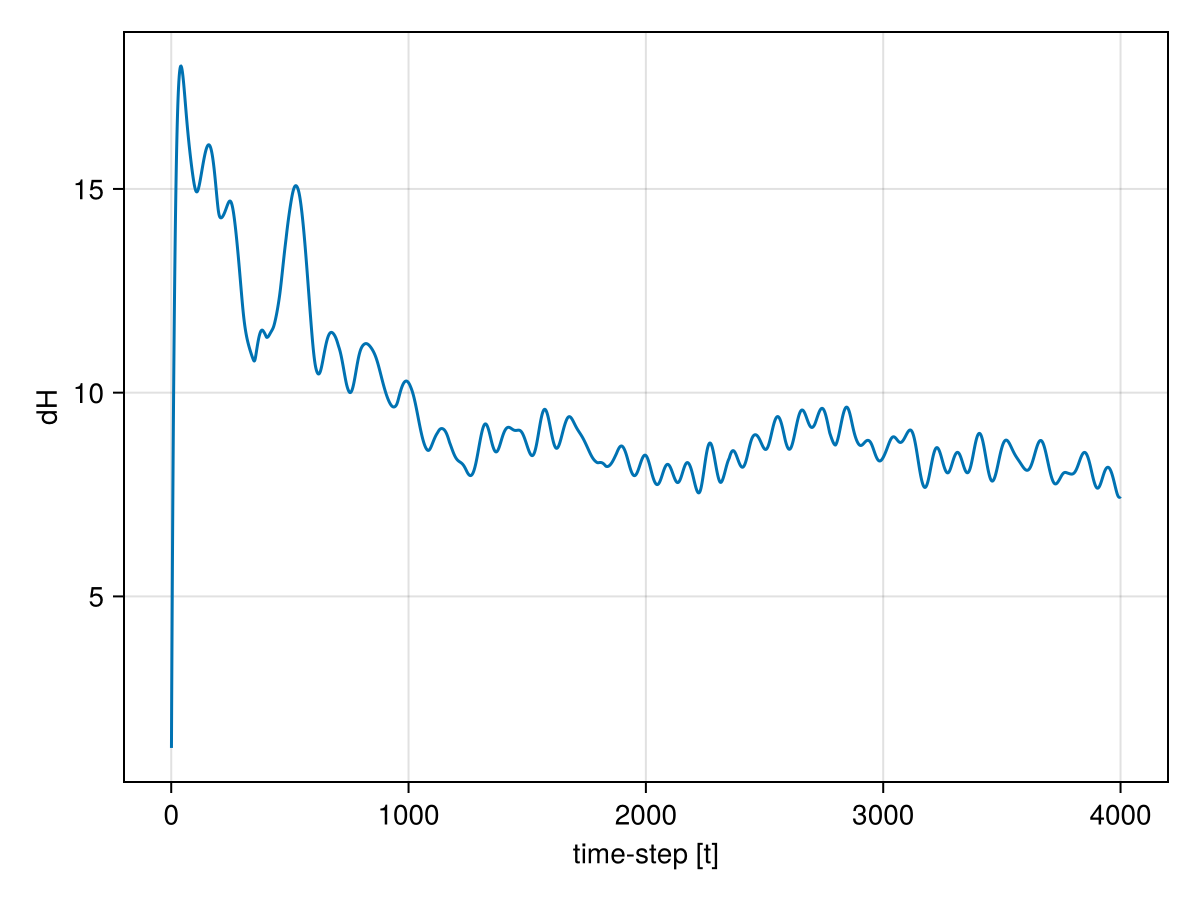
\includegraphics[width=\linewidth]{figures/dH_cross2.png}
            \caption{Time derivative of Hamiltonian $\frac{d}{dt}H$}
            \label{plot:cross2_dh}
        \end{subfigure}
        \caption{Stripe formation at a diagonal for cross flow with $\lambda = 2$}
        \label{plot:cross2}
    \end{figure}
Starting from the same positions as \autoref{plot:starting_pos} with the desired velocities set to $u_i = \begin{bmatrix} 1 & 0 \end{bmatrix}$ for half of the pedestrians (Green), and $u_i = \begin{bmatrix} 0 & 1 \end{bmatrix}$ for the other half (Red). We can observe that the pedestrians form a \textit{diagonal} stripe formation; they are not able to reach the desired direction with much ease, forming an angled trajectory. This is also apparent when we look at the plots for the Hamiltonian, as the $\frac{d}{dt}H$ fluctuates over time. However, the long term dynamics of the pedestrians would result in an arrangement where the pedestrians don't deviate from their desired directions, as shown in the next case.

\pagebreak
    \item \textbf{Stripe Formation for cross flow with $\lambda = 3$}
    \begin{figure}[H]
        \centering
        \begin{subfigure}{\textwidth}
            \centering
            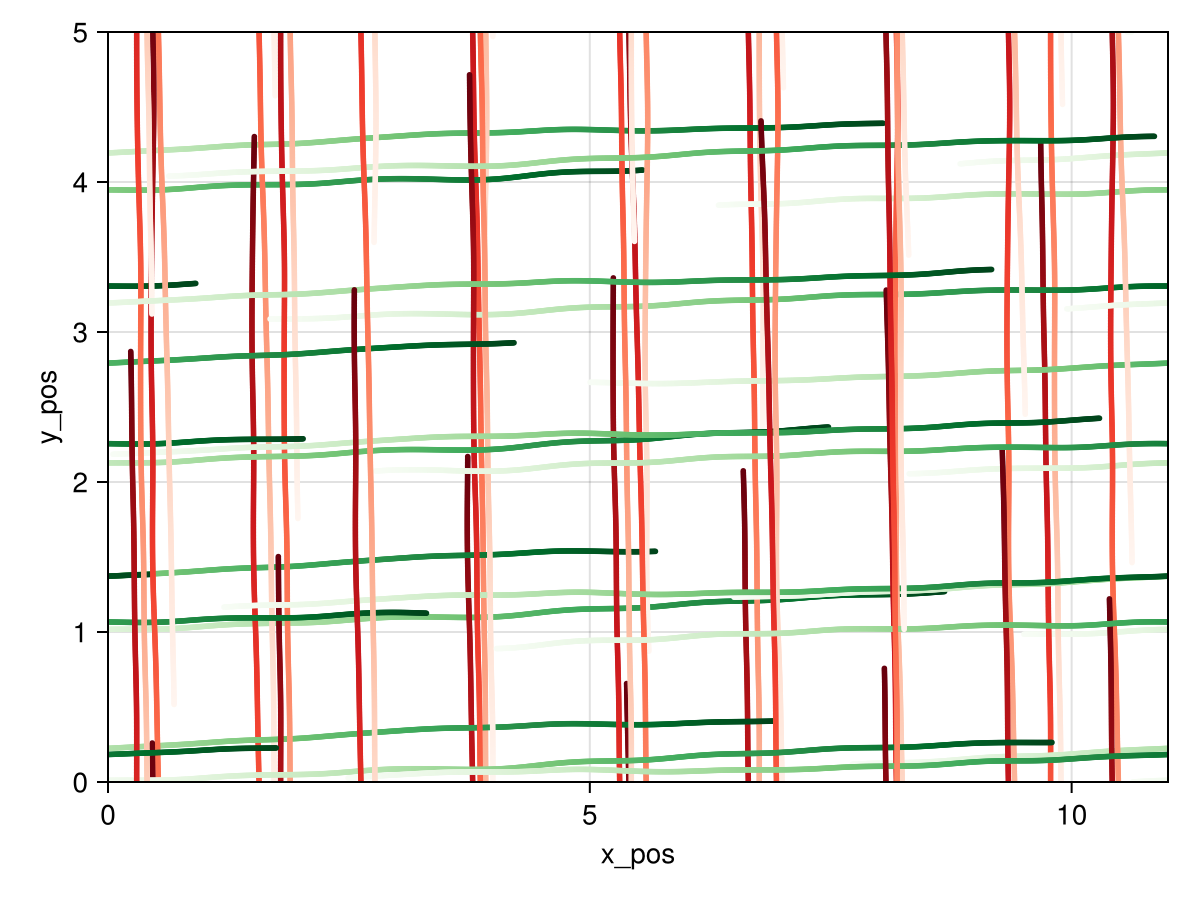
\includegraphics[width=0.6\linewidth]{figures/s0crossleap3flow_10000.png}
            \caption{Pedestrian trajectories}
            \label{plot:cross_traj}
        \end{subfigure}
        \begin{subfigure}{.40\textwidth}
            \centering
            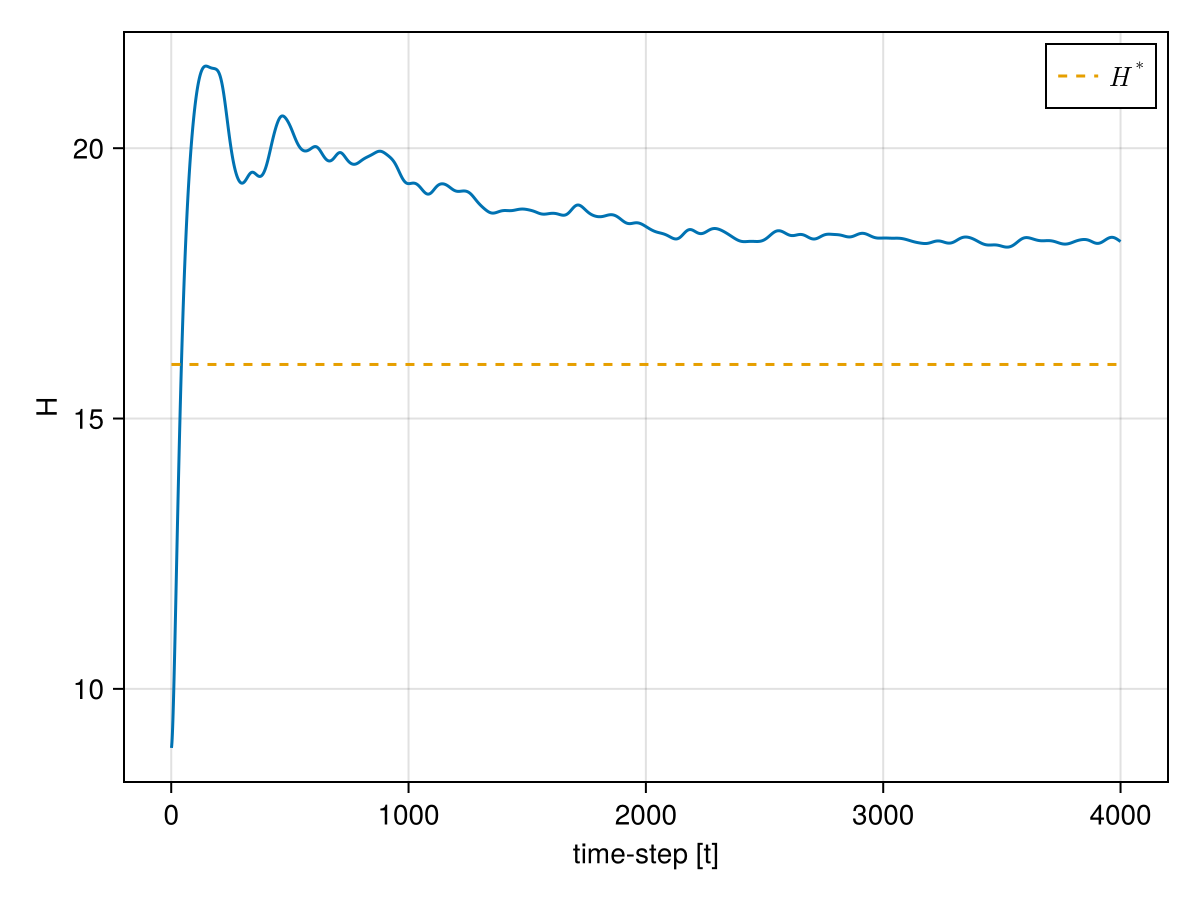
\includegraphics[width=\linewidth]{figures/H_cross.png}
            \caption{Hamiltonian $(H)$}
            \label{plot:cross_h}
        \end{subfigure}
        \begin{subfigure}{.40\textwidth}
            \centering
            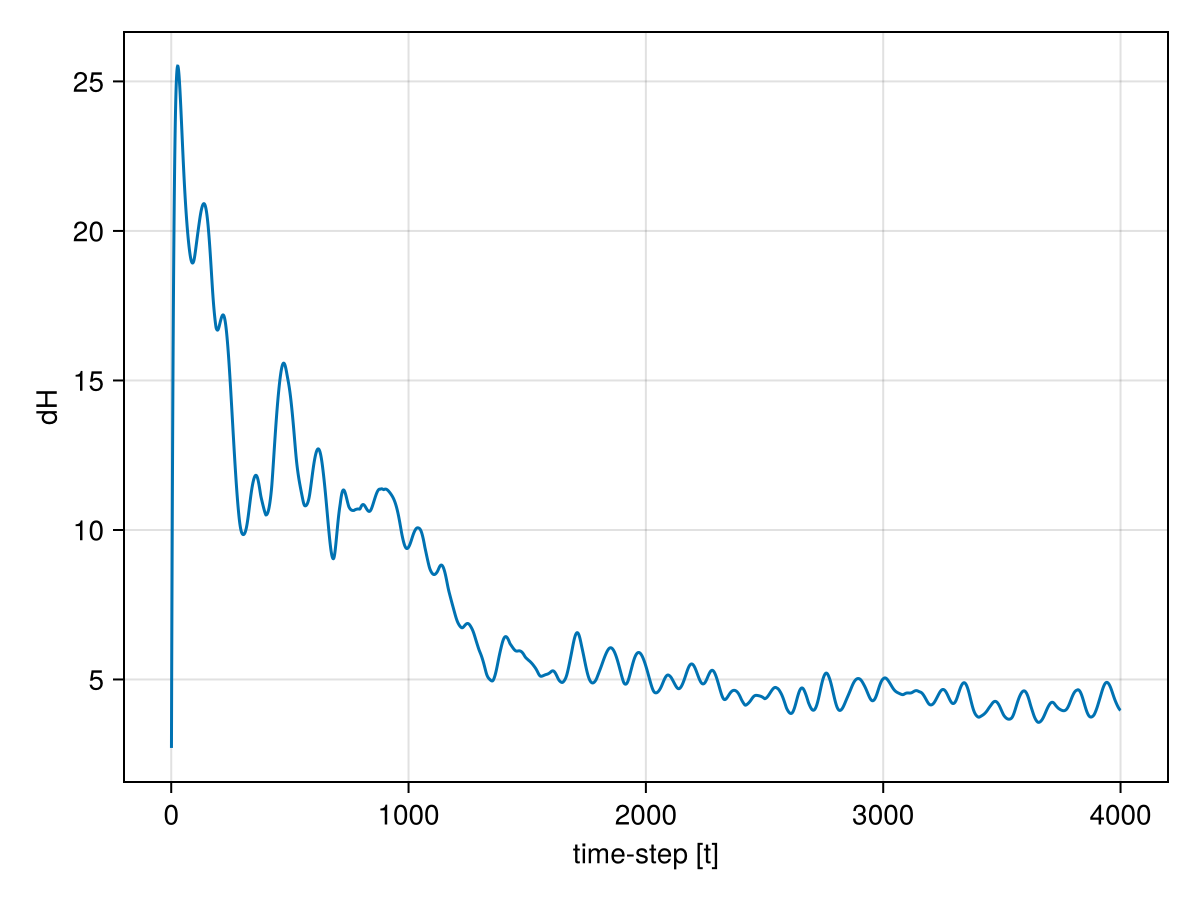
\includegraphics[width=\linewidth]{figures/dH_cross.png}
            \caption{Time derivative of Hamiltonian $\frac{d}{dt}H$}
            \label{plot:cross_dh}
        \end{subfigure}
        \caption{Stripe formation for cross flow with $\lambda = 3$}
        \label{plot:cross3}
    \end{figure}
Here we replicate the model from before, though we set $\lambda$ to a higher value, we can clearly observe a better stripe formation. The Hamiltonian also doesn't fluctuate too much as $\frac{d}{dt}H$ decreases more quickly. In both of these cases, we can observe that the stripe formation occurs, and the Hamiltonian remains above $H^*$
\pagebreak    
    \item \textbf{Gridlock for cross flow with $\lambda = 0.2$}
    \begin{figure}[H]
        \centering
        \begin{subfigure}{\textwidth}
            \centering
            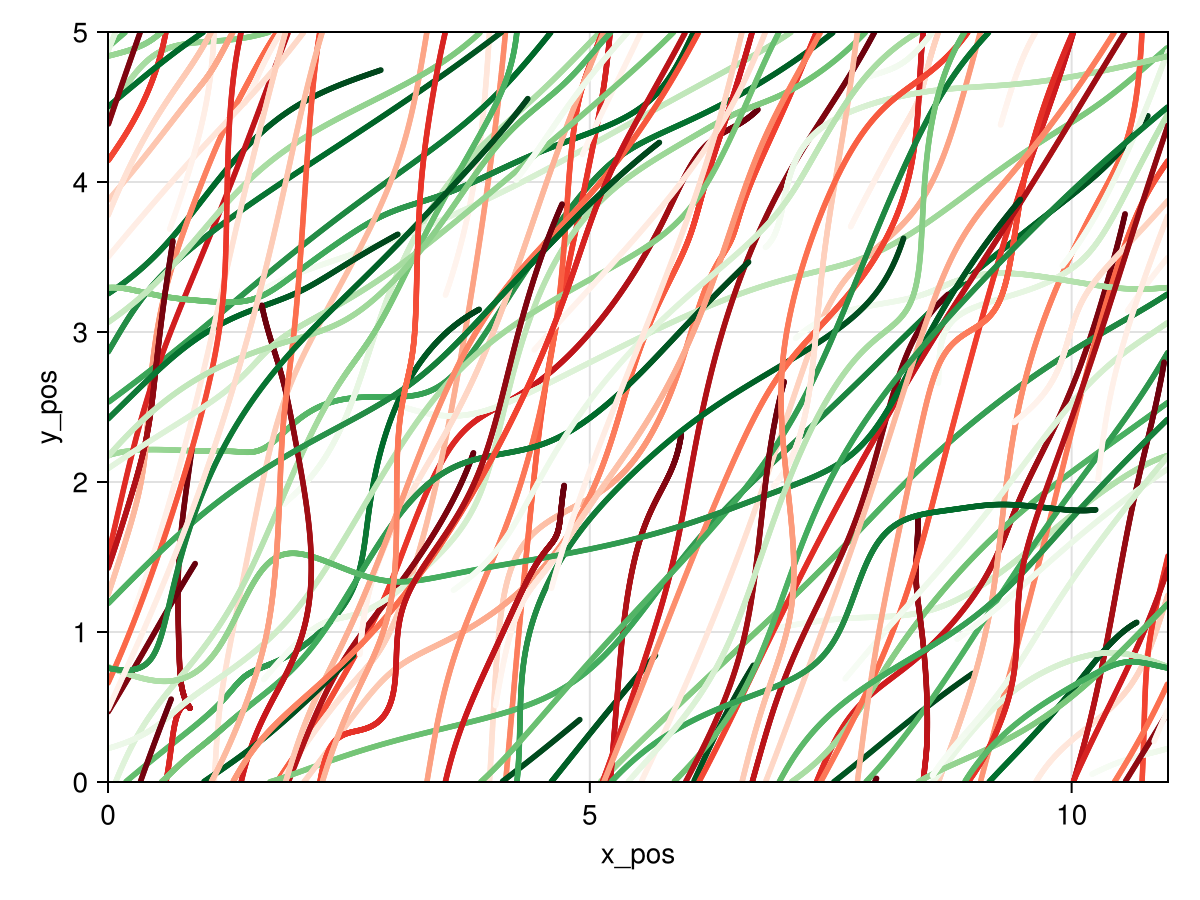
\includegraphics[width=0.6\linewidth]{figures/cross_gridlockdflow_4000.png}
            \caption{Pedestrian trajectories}
            \label{plot:crossgridlock_traj}
        \end{subfigure}
        \begin{subfigure}{.40\textwidth}
            \centering
            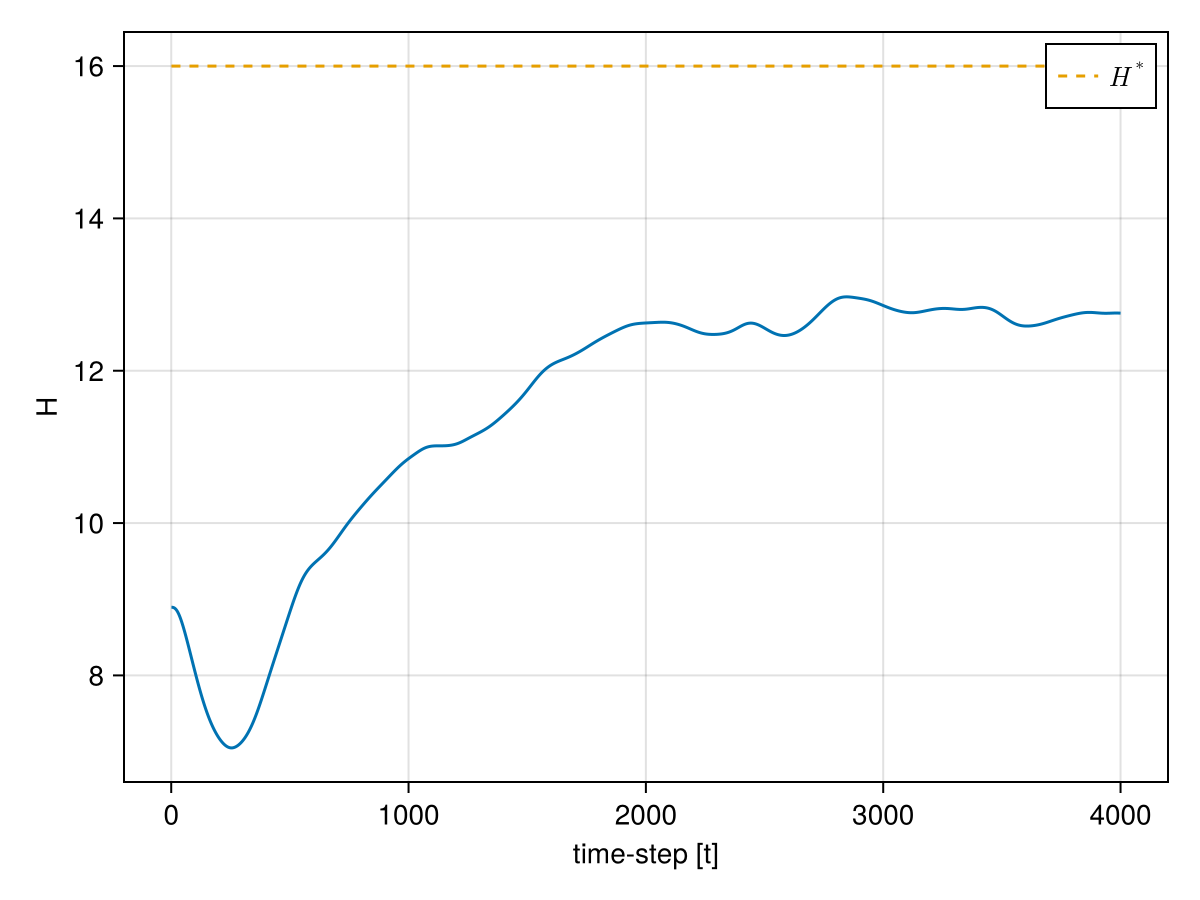
\includegraphics[width=\linewidth]{figures/H_cross_gridlock.png}
            \caption{Hamiltonian $(H)$}
            \label{plot:crossgridlock_h}
        \end{subfigure}
        \begin{subfigure}{.40\textwidth}
            \centering
            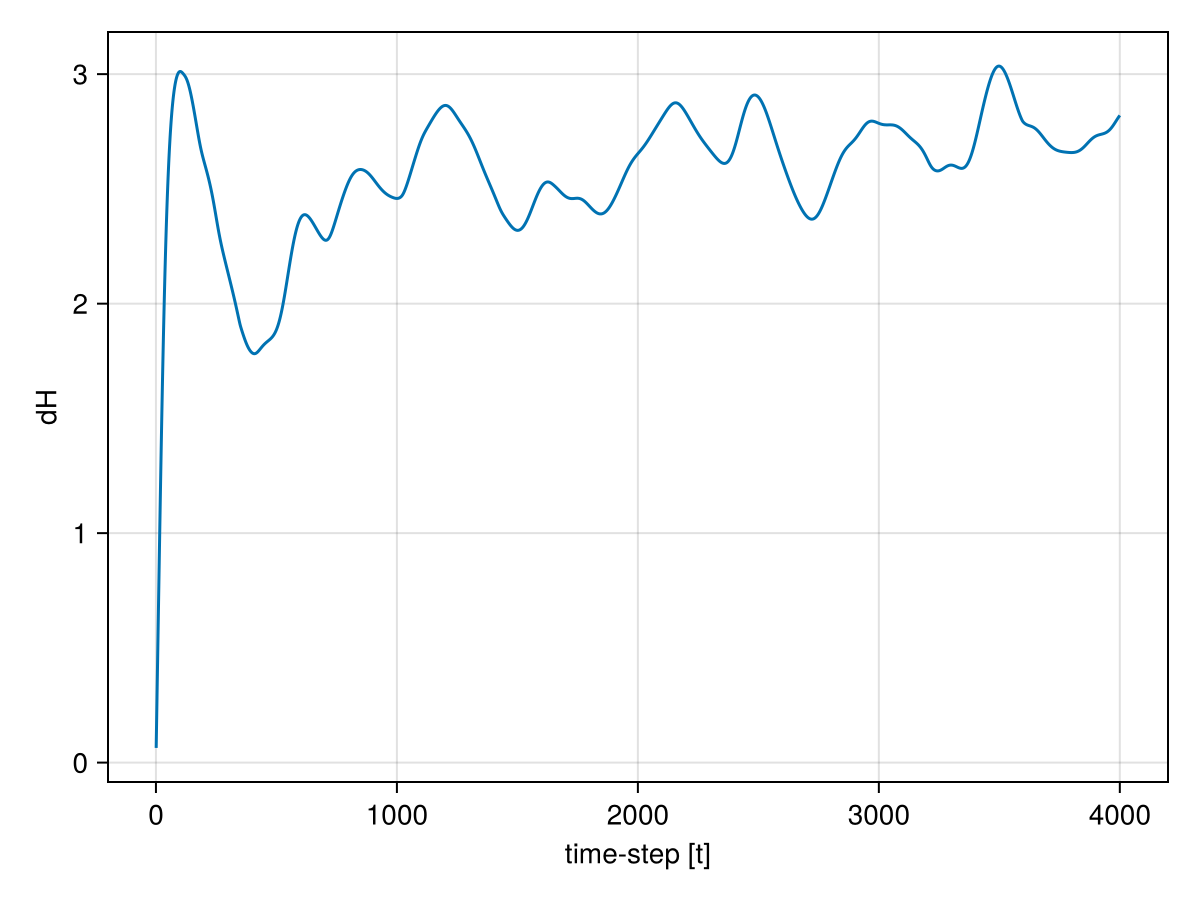
\includegraphics[width=\linewidth]{figures/dH_cross_gridlock.png}
            \caption{Time derivative of Hamiltonian $\frac{d}{dt}H$}
            \label{plot:crossgridlock_dh}
        \end{subfigure}
        \caption{Gridlock for cross flow}
        \label{plot:crossgridlock}
    \end{figure}
Here we can see that no stripe formation occurs, as $\lambda$ is not high enough for the pedestrians to be reactive. The Hamiltonian also remain below $H^*$
\end{itemize}

From the simulations above, we have observed that collective dynamics occur when the Hamiltonian remains above $H^*$. 
\pagebreak
\subsection{Stochastic Model Dynamics}
In this section, we once again pay our attention to the stochastic model dynamics. We will keep the same parameters as \autoref{code:model_init}, and focus mainly on three cases: unidirectional, counter, and cross flows. In all of these cases, we will increase the volatility $\sigma$ for every simulation. In a physical sense, one can interpret the addition of noise as 'warming' the system, and hence we will notice, for most cases, that the overall energy of the systems increase with increase in noise. We observe the long term dynamics and also the rate of change of Hamiltonian $\frac{d}{dt}H$ over time.

\begin{itemize}
    \item \textbf{Unidirectional flow ($\sigma \geq 0$)}
    \begin{figure}[H]
        \centering
        \begin{subfigure}{.49\textwidth}
            \centering
            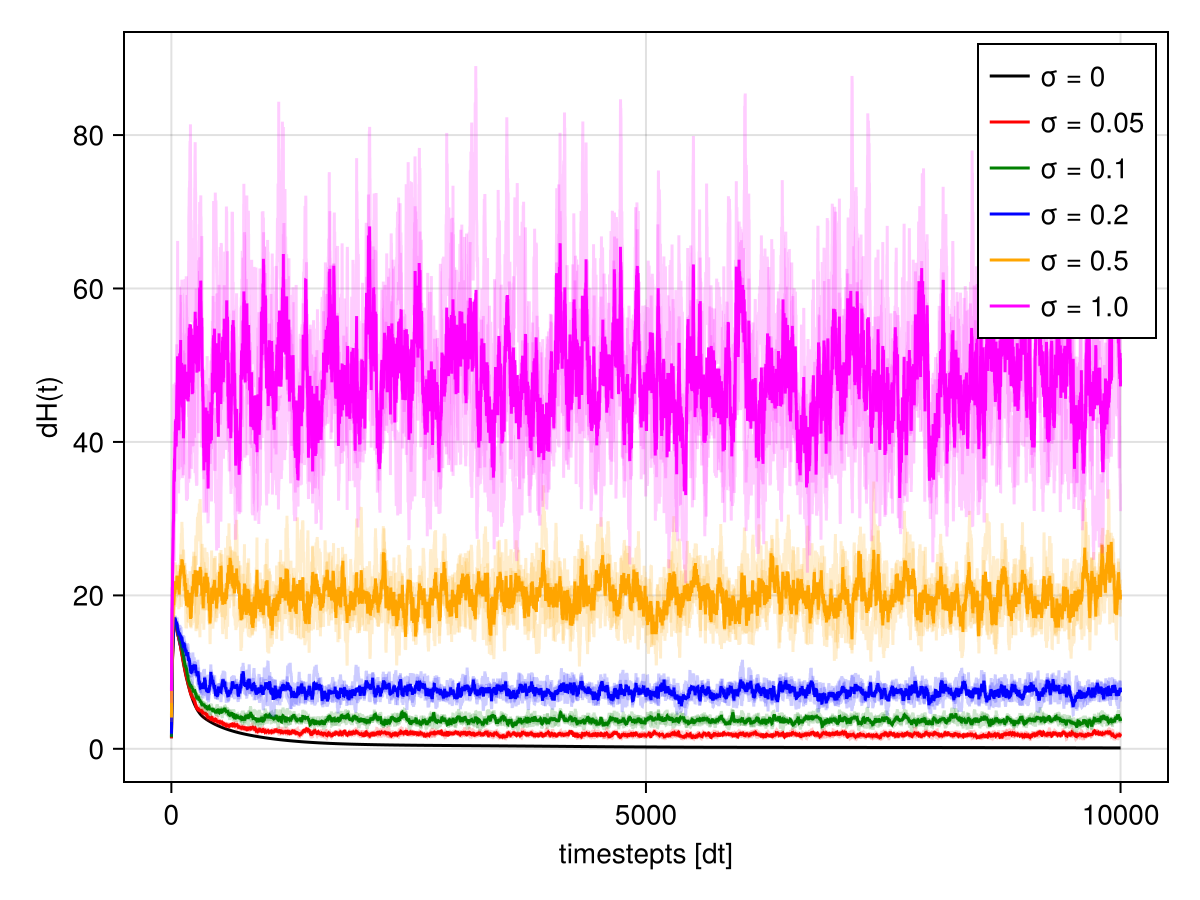
\includegraphics[width=\linewidth]{figures/dH_stochasic_uni.png}
            \caption{$\frac{d}{dt}H(t)$ over time}
            \label{plot:stoc_uni_dh}
        \end{subfigure}
        \begin{subfigure}{.49\textwidth}
            \centering
            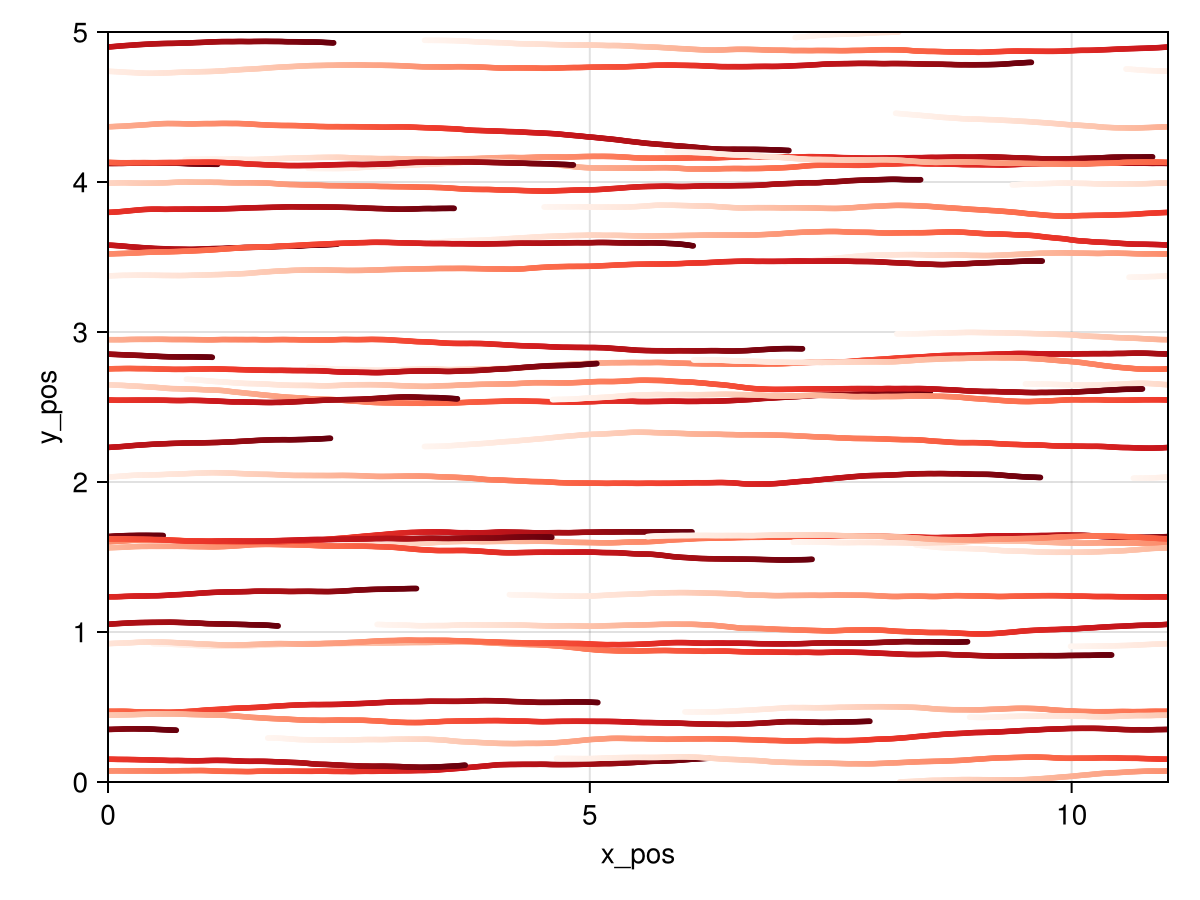
\includegraphics[width=\linewidth]{figures/st_unidflow_5000.png}
            \caption{Pedestrian trajectories for $\sigma = 0.05$}
            \label{plot:stoc_uni_traj}
        \end{subfigure}
        \caption{Unidirectional flow with stochastic effects}
        \label{plot:stoc_uni}
    \end{figure}
    With $\sigma = 0$ being the deterministic case, and $\sigma > 0$ as the non-deterministic cases. We can observe that increasing the volatility in the dynamics perturbs the velocity of the pedestrians in the unidirectional case. The effects of the randomness are as expected; the dynamics deviate more when the volatility is high.
    \pagebreak
    \item \textbf{Cross flow ($\sigma \geq 0$)}
    \begin{figure}[H]
        \centering
        \begin{subfigure}{.49\textwidth}
            \centering
            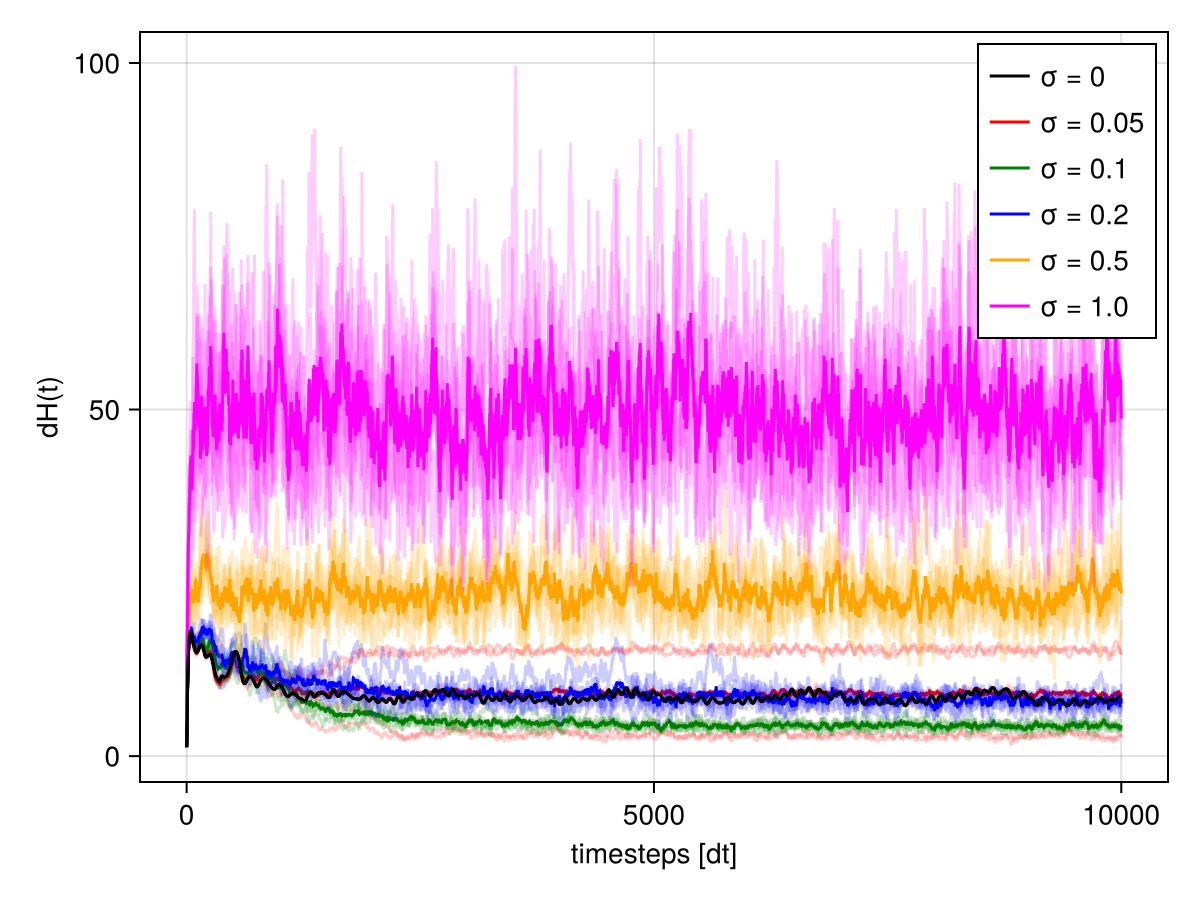
\includegraphics[width=\linewidth]{figures/dH_stochasic_cross_sigmaxy.png}
            \caption{$\frac{d}{dt}H$ over time}
            \label{plot:stoc_cross_dh}
        \end{subfigure}
        \begin{subfigure}{.49\textwidth}
            \centering
            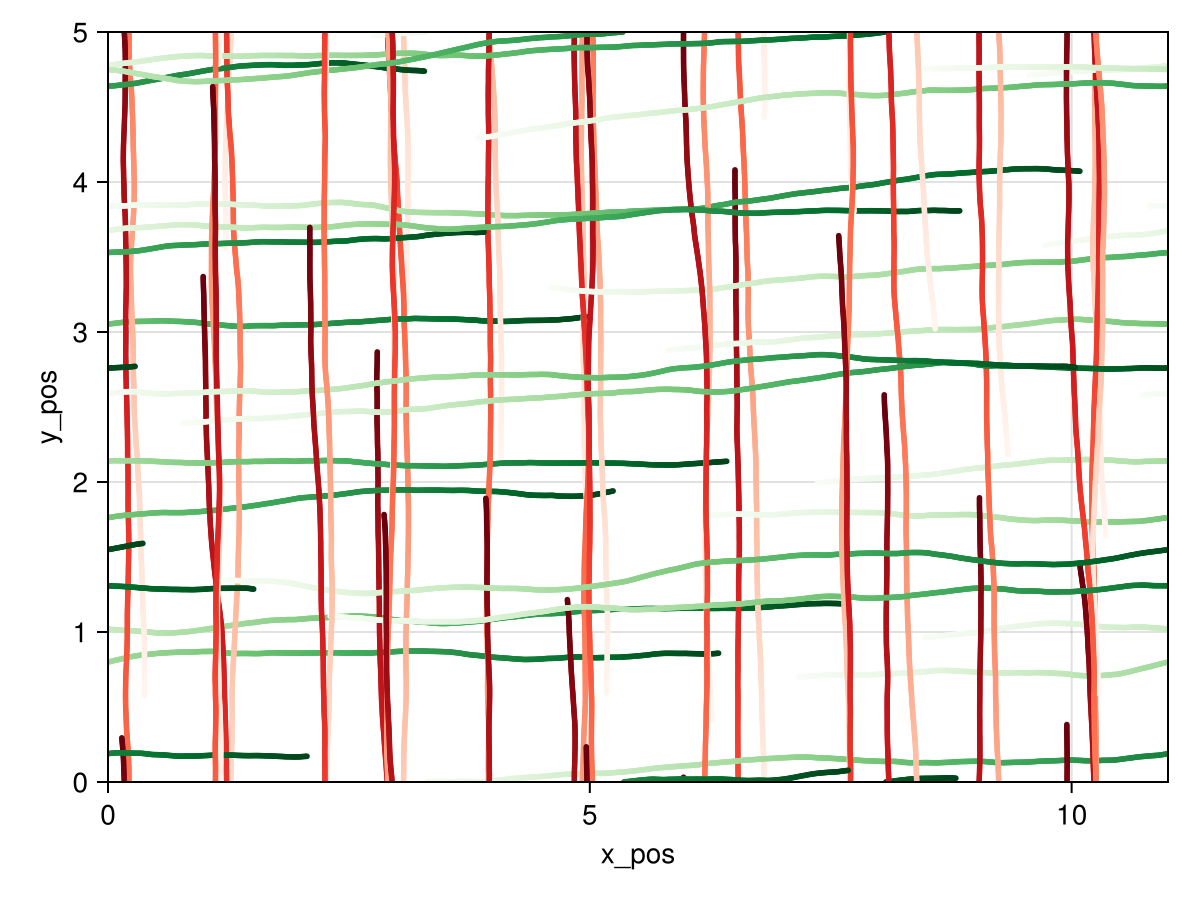
\includegraphics[width=\linewidth]{figures/s0.1_crossflow_10000.png}
            \caption{Pedestrian trajectories for $\sigma = 0.1$}
            \label{plot:stoc_cross_traj}
        \end{subfigure}
        \caption{Cross flow with stochastic effects, showing that the stripe formation improves with noise levels $\sigma \leq 0.2$}
        \label{plot:stoc_cross}
    \end{figure}
    For cross flows, the stochastic dynamics produce interesting results. For smaller values of $\sigma\geq 0$, the change of rate of the Hamiltonian is even less than the deterministic case. For such values $\sigma \leq 0.2$, as indicated in \cite{khelfa2021initiating}, the trajectories of the pedestrians also show that the stripe formation is improved with the addition of noise in contrast to its deterministic counterpart \autoref{plot:cross2}. This counterintuitive phenomenon for the stochastic cross flow is known as 'noise-induced ordering' \cite{d2021canard}. However, this stripe formation is disrupted with increase in noise, particularly for values $\sigma \geq 0.5$
    \item \textbf{Counter flow ($\sigma \geq 0$)}
    \begin{figure}[H]
        \centering
        \begin{subfigure}{.49\textwidth}
            \centering
            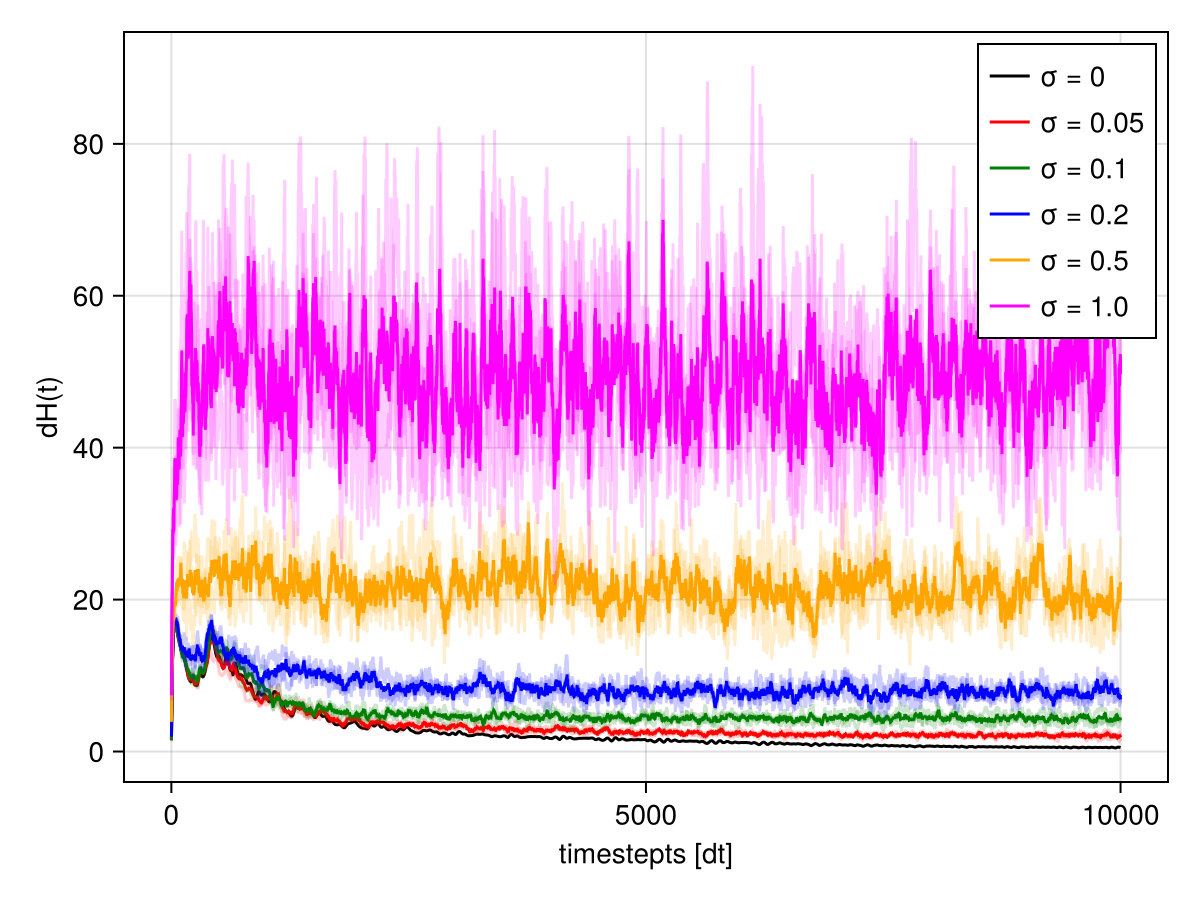
\includegraphics[width=\linewidth]{figures/dH_stochasic_counter.png}
            \caption{$\frac{d}{dt}H$ over time}
            \label{plot:stoc_counter_dh}
        \end{subfigure}
        \begin{subfigure}{.49\textwidth}
            \centering
            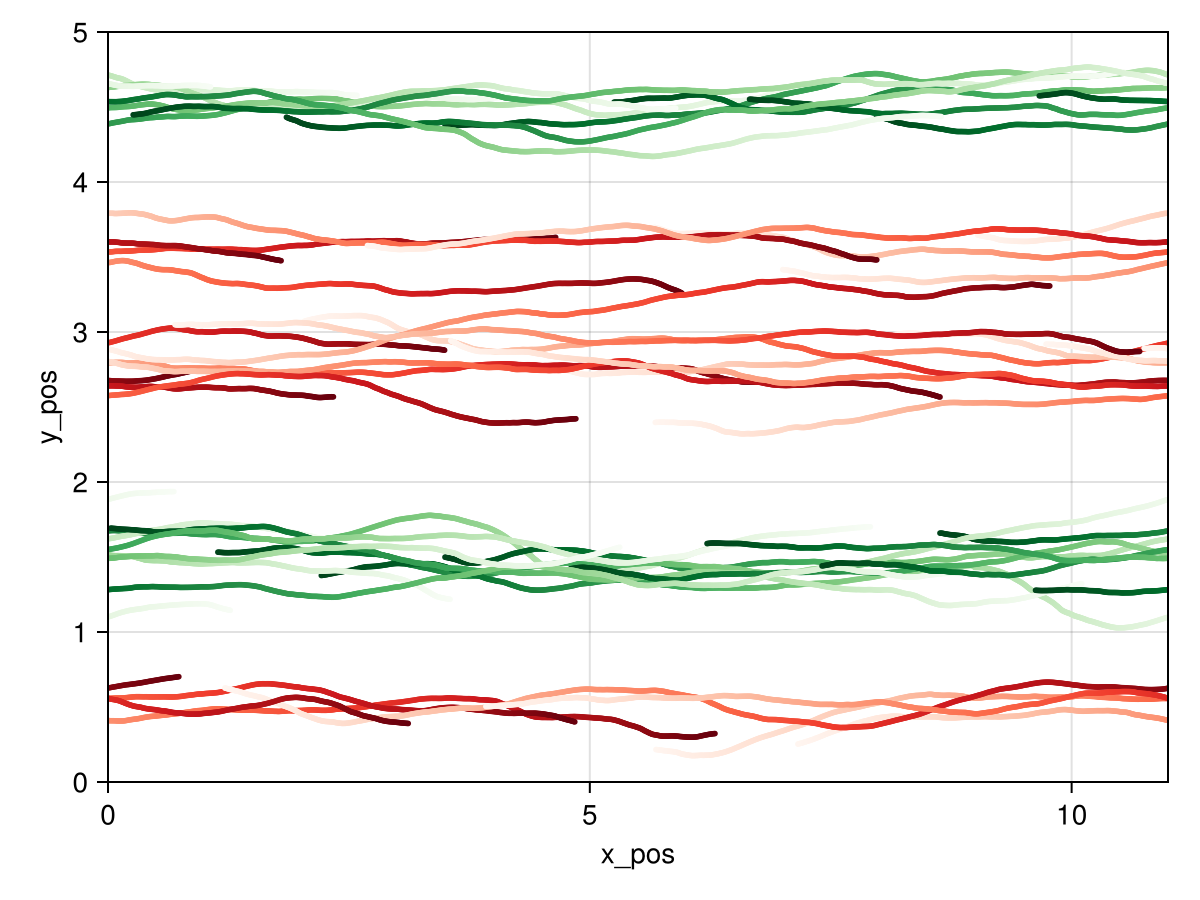
\includegraphics[width=\linewidth]{figures/s0.2_counterflow_10000.png}
            \caption{Pedestrian trajectories for $\sigma = 0.2$}
            \label{plot:stoc_counter_traj}
        \end{subfigure}
        \caption{Counter flow with stochastic effects}
        \label{plot:stoc_counter}
    \end{figure}
    In the case of the counter flow, however, we do not see an improvement in lane formation with addition of noise in the system. The lane formation is perturbed with the increase in noise and becomes indistinguishable from disordered movement when $\sigma \geq 0.5$. As the velocities of the pedestrian is decreasing here, it can be noted that this an onset of a phenomenon known as 'freezing by heating' \cite{helbing2000freezing}.
\end{itemize}

All the dynamics shown in this section, have the overall Hamiltonian greater than $H^*$, however the collective dynamics does not necessarily occur even when this condition is met in the stochastic cases, specially for the cases with high levels of noise. This could be because the rate of change of the Hamiltonian $\frac{d}{dt}H$ rapidly fluctuates, indicating erratic movement of the overall dynamics of the agents, resulting in no phase changes from disordered to ordered dynamics.



\pagebreak
\section{Complete Coding Examples}
In this section we show coding examples to demonstrate to the reader how to set up a complete model. As we move on, we'll gradually add more customization options to our model setup to have more flexibility. We'll also show how to save and plot data obtained from our simulation, e.g. the pedestrians attributes such as positions and velocity, and also model attributes such as the Hamiltonian. The only files that we will be using from the root project directory are:
\begin{itemize}
    \item \texttt{/activate\_package.jl}
    \item \texttt{/PH\_Project/src/module\_ph\_ped.jl}
\end{itemize}
As we will see in our example, the very first step to start a project would always be to activate the package by executing \texttt{activate\_package.jl}. For any advanced customization, for e.g. changing the numerical solver for the \texttt{stochastic\_ode\_step}, we will have to manually modify the function \autoref{code:sde_solve} within the \texttt{module\_ph\_ped.jl}.

\subsection{Model Setup}
To begin with our examples, let us create a new julia file \texttt{/main.jl} and activate our package.

\begin{listing}[H]
\begin{minted}[escapeinside=??,frame=single, fontsize=\small]{julia}
include("./activate_package/activate_package.jl")
\end{minted}
\end{listing}

\subsubsection*{Example 1: Minimal model setup with default parameter values}
\begin{listing}[H]
\begin{minted}[escapeinside=??,frame=single, fontsize=\small]{julia}
model = initialize()
\end{minted}
\caption{Minimal code to construct a model with default parameter values}
\label{code:ex1}
\end{listing}
With a simple command shown above \autoref{code:ex1}, we can easily construct and initialize the model with default values. We've initialized the model with 32 pedestrians, in the space of 11 units and 5 units in the x and y directions respectively. To retrieve model properties, for e.g. \texttt{λ}, we can write \texttt{model.λ}. Similarly, for agent properties, we can write \texttt{model[1].pos} to retrieve the position of the agent with index 1.
\begin{listing}[H]
\begin{minted}[escapeinside=@@,frame=single, fontsize=\small]{shell-session}
StandardABM with 32 agents of type Pedestrian
agents container: Vector
space: periodic continuous space with [11.0, 5.0] extent and spacing=0.25
scheduler: fastest
properties: no_disp_H, A, λ, B, dH, dt, sigma, alignment, stoch_dH, 
hamiltonian    
\end{minted}
\caption{Output of \autoref{code:ex1} in the terminal, showing model initialization with default values.}
\label{code:repl_ex1}
\end{listing}

\subsubsection*{Example 2: Model setup with user-defined parameter values}
\label{section:ex2}

\begin{listing}[H]
\begin{minted}[escapeinside=@@,frame=single, fontsize=\small]{julia}
seed = 42
properties = Dict(
    # constants
    :λ => 2, :A => 5, :B => 0.3, :dt => 0.01, :sigma => 0.1,
    # hamiltonian and alignment
    :no_disp_H => 0.0, :hamiltonian => 0.0, :dH => 0.0, :stoch_dH => 0.0,
    :alignment => 0.0
)
number_of_peds = 0
x_len, y_len = 11, 5
num_solver = leapfrog_step
\end{minted}
\caption{Initializing model parameters}
\label{code:ex2}
\end{listing}

If we wish to have flexibility in initializing the model parameters beforehand, we can do that by simply writing the arguments as shown in \autoref{code:ex2} for the \texttt{initialize} function \autoref{code:ex2-1}.
\begin{listing}[H]
\begin{minted}[escapeinside=@@,frame=single, fontsize=\small]{julia}
model = initialize(
    number_of_peds, x_len, y_len, num_solver, properties; seed
    )
\end{minted}
\caption{Initialization of the model with modified parameters from \autoref{code:ex2}}
\label{code:ex2-1}
\end{listing}
As we have created the model with zero pedestrians, we can now manually add the pedestrians into our model space using \texttt{addagent!()} as shown below \autoref{code:ex2-2}, and initialize their attributes.

\begin{listing}[H]
\begin{minted}[escapeinside=@@,frame=single, fontsize=\small]{julia}
rng = Distributions.Xoshiro(seed)
number_of_peds = 40
for i in 1:number_of_peds
    Agents.add_agent!(model;
        pos = [rand(rng)*x_len, rand(rng)*y_len],  # Initial position
        vel = [0.0 ,0.0], # Initial velocity
        u@\sub{i}@ = mod(i,2) == 0 ? [1,0] : [-1,0] # counter_flow
        # u@\sub{i}@ = mod(i,2) == 0 ? [0,1] : [1,0] # cross
        # u@\sub{i}@ = [1.0,0.0] # uni-directional flow
    )
end
\end{minted}
\caption{Initialization of the pedestrians}
\label{code:ex2-2}
\end{listing}

The \texttt{addagent!()} function adds a \texttt{Pedestrian} object as an agent into our model. The attributes of \texttt{Pedestrian} were defined in \autoref{code:agent_def}, and hence \texttt{vel}, \texttt{pos}, and \texttt{u\sub{i}} are initialized in \autoref{code:ex2-2}.
    
\subsection{Running the Model}
Once we are satisfied with our model, the next step is to run it! Naturally, we would also want to keep track of how the model and agent attributes change as the simulation runs. Continuing with the model defined in Example 2, we'll run this model for 100 seconds of simulation time, and save the values of each attribute in the \texttt{adf} and \texttt{mdf} dataframes.

\begin{listing}[H]
\begin{minted}[escapeinside=@@,frame=single, fontsize=\small]{julia}
T = 100
total_steps = T/model.dt # or T/properties[:dt]
mdata = [:hamiltonian, :dH, :no_disp_H, :alignment, :stoch_dH]
adata = [:pos, :vel]
adf, mdf = Agents.run!(model, T; mdata, adata)
\end{minted}
\caption{Running the model and tracking the attributes}
\label{code:ex2-run}
\end{listing}

Here, \texttt{mdf} is a dataframe containing a record of the changes over time of all model attributes declared in \texttt{mdata}, similarly the agents attributes declared in \texttt{adata} are saved in the \texttt{adf} dataframe.

\subsubsection*{Visualizing Model Data}
Once the simulation is finished and the dataframes are obtained, we can easily analyze them. As an example, we will illustrate how we can plot the data, and finally show how we can construct a simple interactive application to simulate our model.

Continuing with the dataframes obtained in \autoref{code:ex2-run}, we will plot them using the \texttt{CairoMakie} backend.
\begin{listing}[H]
\begin{minted}[escapeinside=@@,frame=single, fontsize=\small]{julia}
t = model.dt:model.dt:T
h_data, h_star_data = mdf[2:end,:hamiltonian] , mdf[2:end,:no_disp_H]

CairoMakie.activate!()
fig, ax = lines(t, h_data)
lines!(ax, t, h_star_data, linestyle=:dash, label=L"H^*")

ax.ylabel = "H"
ax.xlabel = "time [s]"
ax.title = "Hamiltonian for counter flow | n = $number_of_peds"
axislegend()
fig
\end{minted}
\caption{Example code to plot model attributes}
\label{code:ex2-mplot}
\end{listing}

Here, we have ignored the data from the first step as it only contains the initialized values of the model. By executing \autoref{code:ex2-mplot}, we'll obtain the following plot \autoref{plot:ex2-mplot}

\begin{figure}[H]
    \centering
    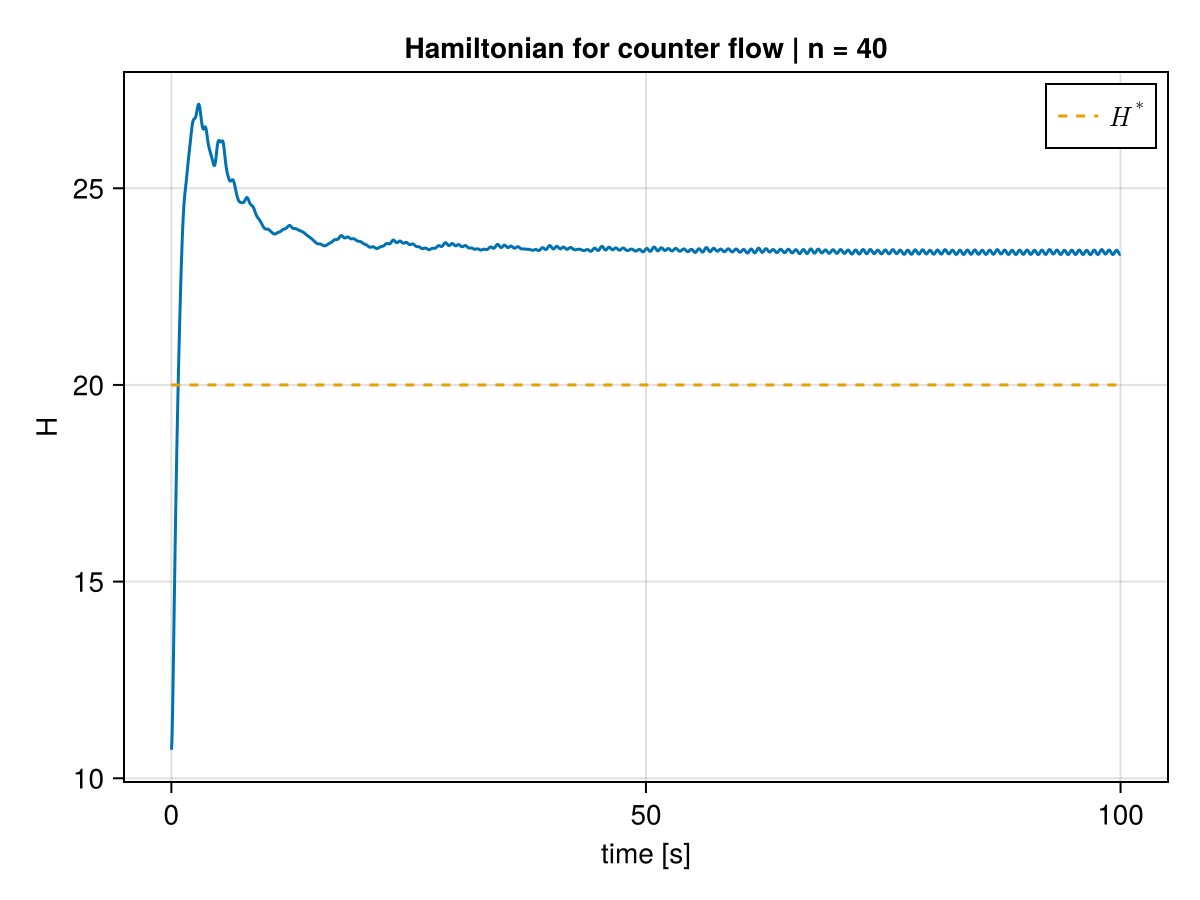
\includegraphics[width=0.5\textwidth]{figures/ch6_tutorial/example_plot.png}
    \caption{Model attribute plot from executing \autoref{code:ex2-mplot}}
    \label{plot:ex2-mplot}
\end{figure}

\subsubsection*{Visualizing Agent Trajectories}
To plot the trajectories of every agent, we use the agent dataframe \texttt{adf} obtained from \autoref{code:ex2-run}. We loop through each \texttt{agent.id} and take its positions within a certain time. Since we have simulated a counter flow \autoref{code:ex2-2}, it would be nice to have a clear distinction between the two groups of agents based on their desired velocities, hence we color them individually.
\begin{listing}[H]
\begin{minted}[escapeinside=@@,frame=single, fontsize=\small]{julia}
path_length = 100
start_time = Int(T/model.dt) - path_length
end_time = start_time + path_length
fig = Figure()
ax = Axis(fig[1, 1], 
          limits = (0,x_len,0,y_len), 
          xlabel = "x_pos", ylabel = "y_pos")
for i in 1:number_of_peds
    if mod(i,2) == 0
        scatter!(ax, adf[adf.id .== i, :].pos[start_time:end_time], 
                color=0:path_length, colormap=:Reds, markersize=5)
    else
        scatter!(ax, adf[adf.id .== i, :].pos[start_time:end_time], 
                color=0:path_length, colormap=:Greens, markersize=5)
    end
end
fig
\end{minted}
\caption{Example code to plot agent trajectories}
\label{code:ex2-aplot}
\end{listing}
We want to see the trajectories of all agents through the 100 timesteps of the simulation. We first set the figure and axis to a defined extent based on the simulation domain that we've defined in \autoref{code:ex2}. Then loop through \texttt{adf}, to get the agent trajectories of each agent. Executing the code results in the plot below

\begin{figure}[H]
    \centering
    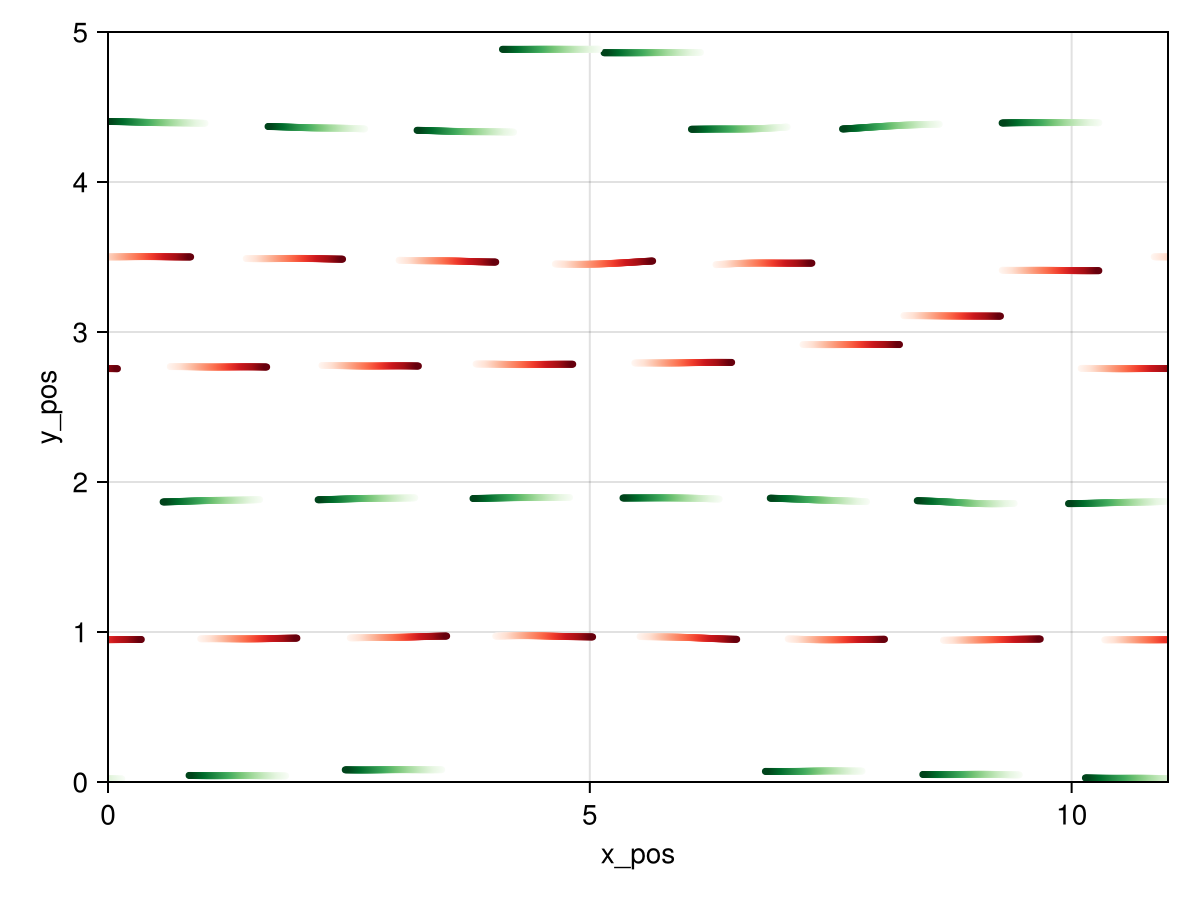
\includegraphics[width=0.5\textwidth]{figures/ch6_tutorial/example_traj.png}
    \caption{Agent trajectories from executing \autoref{code:ex2-aplot}}
    \label{plot:ex2-aplot}
\end{figure}


\subsection{Interactive Visualization}
To construct an interactive application, we'll use the \texttt{GLMakie} backend. Since we want to restart the model every time we open the app, we will initialize the model beforehand, thus we will combine all the codes from example 2 into one function \texttt{model\_init} which will return the initialized model.

To ignore the first initialized values when plotting the data, we run the model for a single time-step using \texttt{Agents.step!(model)}. 
\begin{listing}[H]
\begin{minted}[escapeinside=@@,frame=single, fontsize=\small]{julia}
GLMakie.activate!()
model = model_init()
Agents.step!(model)
params = Dict(
    :λ => 0:0.1:5,
    :A => 0:0.1:10,
    :B => 0:0.1:2,
    :sigma => 0:0.05:1
)
mdata = [:hamiltonian, :dH, :alignment]
fig, abmobs = Agents.abmexploration(model; dt=1:0.2:5, params, mdata)
fig
\end{minted}
\caption{Example code to generate the interactive app}
\label{code:ex2-app}
\end{listing}

Sliders can also be added by creating a dictionary with key value pairs of the model attributes with step ranges shown in \autoref{code:ex2-app}. Finally, to generate the plots of the attributes, we can include \texttt{mdata} with a list of attributes to track, similar to how it was done when running the model in \autoref{code:ex2-run}. With these arguments in \texttt{Agents.abmexploration}, one can create a simple interactive GUI as shown below in \autoref{fig:ex2-app}.

\begin{figure}[H]
    \centering
    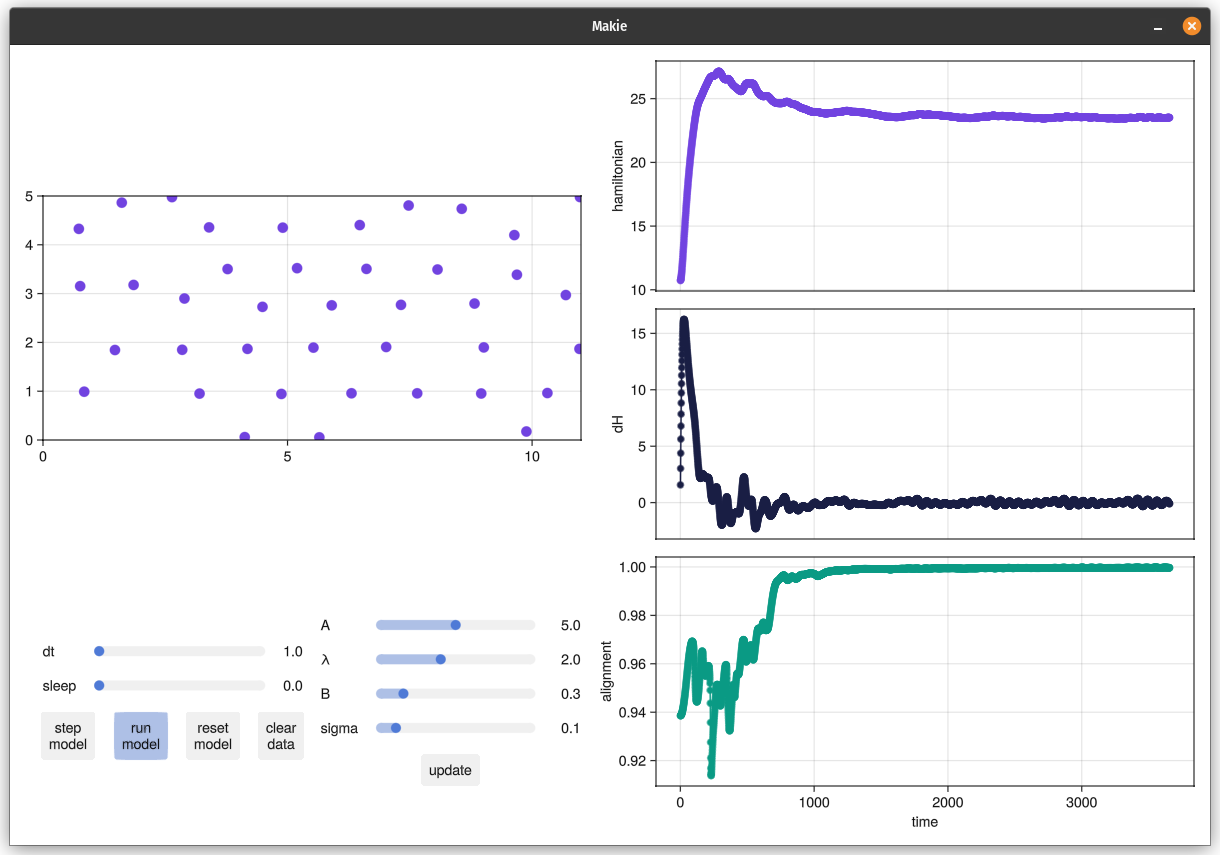
\includegraphics[width=\textwidth]{figures/ch6_tutorial/example_app1.png}
    \caption{Interactive application to simulate the model by executing \autoref{code:ex2-app}}
    \label{fig:ex2-app}
\end{figure}

Of course, with the ease and flexibility provided by the \texttt{Agents.jl} package, one can easily construct more customizable agent based models apps without hassle.

In this section we demonstrated how to easily construct and run our model, we saved and plotted the model and agent data, and finally we also saw how to create an interactive environment to simulate our model with just a few lines of code.
\pagebreak
\section{Conclusion}

We were successfully able to show the microscopic force-based pedestrian dynamics model through port-Hamiltonian formulation. We witnessed a shift in perspective from microscopic models, where we inspect agent interactivity on an individual level; to a holistic description of the system-wide interactivity through measuring the system energy. This energy-based perspective, enabled by port-Hamiltonian systems, allowed us to not only observe collective behavior, but also to identify it through quantitative means using the Hamiltonian and $H^*$. With the port-Hamiltonian formulation, we were able to replicate the findings from \cite{tordeux2022multi} of well-known collective phenomenon such as lane and stripe formation. 

We can also observe that the interaction between the pedestrians is isotropic, this is due to the skew-symmetric nature of Hamiltonian systems. A physical interpretation of this, in the context of our model, assumes that the pedestrians interact equally with all of its surroundings, hence there are no vision cones effects \cite{helbing1995social} that may produce bias in interaction in the direction of motion. An attempt to incorporate such anisotropic effects within the port-Hamiltonian approach includes the use of state-dependent input terms \cite{tordeux2022multi} though it remains an active part of research.

Furthermore, we were also able to show the impact of induced noise on these collective phenomenon, in particular, "noise-induced ordering" for stripe formation \cite{khelfa2021initiating,d2021canard}. In the case of lane formation, the collective phenomenon was disrupted, resulting in slower velocities of agents, which is in accordance with the "freezing by heating" phenomenon \cite{helbing2000freezing}, however formation of the clusters of agents could not be reproduced.

With this thesis, we've been able to show that port-Hamiltonian systems, although a relatively young area of research, promises a modeling approach to quantify collective dynamics. Because it models systems from the perspective of energy-based interactions, it is more abstract, and thus useful to understand the underlying dynamics of systems from to various disciplines.
\newpage
\listoffigures
\listoflistings
% \listoftables



\printbibliography
\end{document}
